\documentclass[11pt]{labbook}
\usepackage[utf8]{inputenc}
\usepackage{graphicx}
\usepackage{csquotes}
\usepackage{float}
\usepackage[margin=1in]{geometry}
\usepackage{setspace}
\usepackage{listings}
\usepackage{color}
\usepackage{array}
\usepackage{xspace}
\usepackage{times}
\usepackage{amssymb, amsmath}
\usepackage{fancyhdr}
\usepackage[]{algorithm}
\usepackage[noend]{algpseudocode}
\usepackage{courier}
\usepackage{subcaption}

\newcolumntype{P}[1]{>{\centering\arraybackslash}p{#1}}

\definecolor{dkgreen}{rgb}{0,0.6,0}
\definecolor{gray}{rgb}{0.5,0.5,0.5}
\definecolor{mauve}{rgb}{0.58,0,0.82}


\textwidth=16.5cm %mikeg: June 18, 2016 - Why is this being set?  It should be set by geometry package

\lstset{frame=tb,
  language=Java,
  aboveskip=3mm,
  belowskip=3mm,
  showstringspaces=false,
  columns=flexible,
  basicstyle={\small\ttfamily},
  numbers=none,
  numberstyle=\tiny\color{gray},
  keywordstyle=\color{blue},
  commentstyle=\color{dkgreen},
  stringstyle=\color{mauve},
  breaklines=true,
  breakatwhitespace=true,
  tabsize=3
}


%%%%%%%%%%%%%%% BEGIN LOCAL COMMANDS %%%%%%%%%%%%%%%%%%%
\newcommand{\DeltaEta}{\ensuremath{\Delta\eta}\xspace}
\newcommand{\DeltaM}{\ensuremath{\Delta M}\xspace}

%%%%%%%%%%%%%%% END LOCAL COMMANDS %%%%%%%%%%%%%%%%%%%


%%%%%%%%%%%%%%% BEGIN LOCAL CUSTOMIZATIONS %%%%%%%%%%%%%%%%%%%
\usepackage{etoolbox}
\makeatletter
%suppress pagebreaks between days
\patchcmd{\addchap}{\if@openright\cleardoublepage\else\clearpage\fi}{\par}{}{}
\makeatother 

%%%%%%%%%%%% END LOCAL CUSTOMIZATIONS %%%%%%%%%%%%%%%%%


\title{Notes for Undergraduate Research Work}
\author{Alan Dixon}

\begin{document}

\labday{June 6, 2016 Notes}

\begin{itemize}
    \item Discovered and fixed two bugs involving an uninitialized selection vector and Mphi values
    \item Said bug fixes resolved the issue of the program crashing around iteration 2500
      
    \item Despite the fixed bugs resolving that issue, log likelihood values still plummet to values eventually reaching 10e-23 which causes the not a number error, causing the MCMC algorithm to halt.
\footnote{mikeg: June 10 2016 --Is this a typo?  Usually it is $\exp{-300}$ that starts to push the limit of numerical precision.
Further, it is unclear to me why this would cause a problem unless you are later converting this number back to a log scale.  
Is it necessary to exponentiate and then take the log?
ANSWER: 10E-23 was user defined.
}
\footnote{mikeg: June 10 2016 --This is confusing given the previous statement. 
  It sounds like you didn't really resolve the underlying issue.
  ANSWER: Problem is now fixed in that the code run, but it seems likely that the bug is still there.}
    \item Due to Newton failing to execute my job request, I had to run the R script on my laptop so I was only able to run it once so more testing is needed but for the meantime it appears it takes until around iteration 42000 for the program to crash.
      \footnote{mikeg: June 10 2016 -- why is newton failing to execute your job requests? 
        How and when will you solve this issue?}
      \footnote{aland: June 27 2016 -- The problem comes from the .SGE scripts. Jeremy Rogers had them tailored to how his directories were set up and where he wanted files to go. Fixing this is pretty low on my priority list since Gauley handles pretty much everything I need to run.}
    \end{itemize}

TODO:\\
    Work on psuedocode\\
    Remove redundancies\\
    Determine if Sphi prior is being used\\
    Improve varialbe names and documentation\\
    Document the R scripts\\
    
\labday{June 7, 2016}

\begin{itemize}
    \item Removed exit statements from FONSEParameter.cpp, PANSEParameter.cpp, and RFPParameter.cpp in order to eliminate warnings when running the check in R
    \item Downloaded all of the necessary files to my Gauley account.
    \item Running FONSE with simulated data and b = 0.001 led to "nan" being reached much more quickly than on my laptop, around iteration 5500.
      \footnote{mikeg: June 10 2016 --is this based on one run on each machine?
        It's more useful to be more quantitative and descriptive} 
    \item Said issue may be a cause of R not working correctly on Gauley as compared to my laptop. 
      Multiple errors and missing packages were encountered. 
      These errors made it impossible to check any plots.
\item{mikeg: If it strange you're running into such errors since gauley is used to develop the code base.
    Are they really errors or, since you execute code, warnings?
    What are the error codes?  
    When discussing errors, it is good to always include some output using the 'quote' or similar environment in \LaTeX.
    Do other people run into these same errors?
  }
    \item Two new Items for the TODO list: Continue troubleshooting R on Gauley and alter Jeremy's .sge scripts so that they no longer email him when I run a job on Newton.
\end{itemize}

\labday{}{June 8, 2016}

\begin{itemize}
    \item Changed the .sge scripts for Newton so that Jeremy no longer receives an email upon the completion of a job.
    \item Changed a function in FONSEModel.cpp to match it's corresponding function in ROCModel.cpp. In particular, I changed a long series of divisions to on division and a series of multiplications because multiplication is a faster operation.
      \footnote{mikeg: June 10 2016 --include the function name. 
        Any information on speed up?
      }
    \item Fixed a typo in the documentation of ROCModel.cpp
    \item Worked out some kink experienced while running R scripts on Gauley. In particular, finally made it so that the plots actually showed up and worked. 
    \item Formulated the hypothesis that the reason we are experiencing a drop in log likelihood comes from a bug involving either deltaM, deltaOmega, or phi after observing the trace plots.
\footnote{mikeg: June 10 2016 --Include plots in your notes, especially if you refer to them, and explain more clearly why you think its behavior indicates this.
}
\end{itemize}


\labday{June 13, 2016}

\begin{itemize}
    \item Fixed an error in FONSEModel.cpp involving a couple of missing semicolons
    \item Fixed an error in the .tex file for the notes where using the hyperref package kept the notes from compiling
    \item After running FONSE again, with simulated data and b = 0.001, it seems the errors in log likelihood are no longer deterministic. Values still plummet, and the traces suggest that both mutation and selection values may be the cause. Further testing and observation is required.
      \footnote{mikeg: June 16, 2016 - If you run the code in serial and set the random number seed, does the behavior become repeatable?}
    \item Found a difference between FONSEModel and ROCModel where ROC would take mutation prior into account and FONSE wouldn't. This might part of the issues causing log likelihood values to plummet, but testing is required.
    \item Uploaded both the new .tex file and its corresponding pdf just in case there's another error that doesn't keep me from compiling on my machine but might keep another from compiling on a different machine.
      \footnote{mikeg: June 16, 2016 - In general, you should refrain from making copies of files (e.g.~labNotes  $\rightarrow$ Lab\_Notes). 
        Instead, rely on the fact that you are using version control and can always revert back or merge with an earlier version of a file.
     }
\end{itemize}

\labday{June 14, 2016}

\begin{itemize}
    \item The addition of the mutation prior into FONSE seems to have stopped the rapid descent of the Log Likelihood values. After running it once with 1000 samples and 1 thining, the log likelihood stayed somewhat stable after starting low and rising to about -20000. The vaules were also similar when running with 1000 samples and 10 thining. More extensive testing is required to ensure that the plummeting problem is finally resolved.
      \footnote{mikeg: June 16, 2016 -
        I am glad that the prior seems to have fixed this problem.  
        I don't understand, however, why it did so.  
        Were the \DeltaM values diverging from the true value substantially?
        Note also that one can relax the effect of the prior by making its $\sigma_\DeltaM$ value large. 
        In fact at the $\lim_{\sigma_\DeltaM \rightarrow \infty}$ the system essentially behaves as if it has a flat prior (which is proportional to 'no prior').
}
        
    \item Although the log likelihood values are starting to come together, there is an issue observed in both the mutation and selection traces where certain codons are not being accepted. 
    \item Conducted further comparisons on FONSE and ROC to remove redundancies and semantic oversight.
\end{itemize}

\labday{June 15, 2016}

\begin{itemize}
    \item After running FONSE overnight, I feel it's safe to conclude that the plummeting log likelihood problem is resolved although there have been issues with multiple, sometimes all but a few, codons with acceptance rates of 0 as backed up by both the output and the trace plots of both mutation and selection, although this is again non deterministic. Running it on Gauley produced far more codons with no impact than when I ran it on my laptop so the non determinism may come from memory or operating system differences.
\footnote{mikeg: June 16, 2016 -
  This shouldn't happen since we are using an MCMC whose step sizes adapt based on the acceptance ratio of the previous samples. 
  (Of course, it would be good to make sure this adaptive option is set.)
  We saw similar 'non-acceptance' behavior with Gabe and/or Jeremy in the past month or two.
  It had to deal with the parameters not being correctly referenced or defined.
  Cedric will remember the details.
}
    \item There was a problem with Gauley involving the machine randomly restarting without being prompted. It doesn't seem like a major problem and the effects seem to be confined to the processes being run on it at the time being prematurely terminated. I'll be keeping an eye for any unespected behavior from Gauley in case the problem ends up being reoccuring.
    \item Studied the model to try and deduce how the simple inclusion of the mutation priors resolved the plummeting problem. So far it still remains fairly unclear and more studying is necessary. 
\end{itemize}

\labday{June 16, 2016}
    \begin{itemize}
        \item Ran FONSE with b = 0.001, samples = 1000, and Thinning = 10 3 separate times. \footnote{mikeg: June 18, 2016- Where all three of these runs carried out with the same set of genes?
If not, then LLik(data$\|$parmeters) surfaces, although similiar, will differ between the runs.
'}
        \item Run 1 \footnote{mikeg: June 18, 2016 - Per my previous request, please include the relevant figures.
        I recommend organizing figures by putting them in a separate folders such as ``Figures/2016/June/16''.
        You should also name them in a consistent manner such as ``FONSE\_run\_1\_trace\_LLik.png''
      }
        \begin{itemize}
          \item Log likelihood settled around -9600
          \item AA's L and R had acceptance rates of 0
          \item stdDevSynthesisRate posterior estimate settled around 1.4, .05 for the proposal width
          \item Trace of the expected values of phi goes to 0.
          \item All codons for L in the mutation traces stop changing and fall out around sample 100 \footnote{mikeg: June 18, 2016 - what does 'fall out' mean?}
          \item R falls out around sample 300
          \item It's the same story for both L and R in the selection traces except it takes about half as many samples for both to fall out
        \end{itemize}
        \item Run 2 \footnote{mikeg: June 18, 2016 - again, figures should be included to help illustrate and document the behavior you describe.}
        \begin{itemize}
            \item Log likelihood settled around -14000
            \item AA's L and R still had acceptance rates of 0 \footnote{mikeg: June 18, 2016 - Have you described this behavior to Cedric? 
                We've seen similar behavior before.}
            \item stdDevSynthesisRate posterior estimate settles around 1.9, .045 for the proposal width
            \item Trace of the log likelihood didn't level off as much. It seemed to still be rising. 
            \item expected phi trace was the same as Run 1
            \item L falls out around the same place in Mutation as Run 1; R falls out twice as fast.
            \item Both fall out twice as fast in the selection traces compared to Run 1.
        \end{itemize}
        \item Run 3
        \begin{itemize}
            \item Log likelihood settled around -20000
            \item AA's L and R still had acceptance rates of 0
            \item stdDevSynthesisRate posterior estimate settled around 2.5, .04 for the proposal width
            \item There was a more pronounced level-off in the log likelihood trace, much like Run 1
            \item expected phi trace leveled off but slightly above 0
            \item Both L and R had mutation and selection traces similar to Run 1
        \end{itemize}
        \item Also worked on documenting FONSE by taking documentation from similar parts in ROC and making the necessary alterations before putting it into FONSE
         
        \begin{figure}
            \centering
            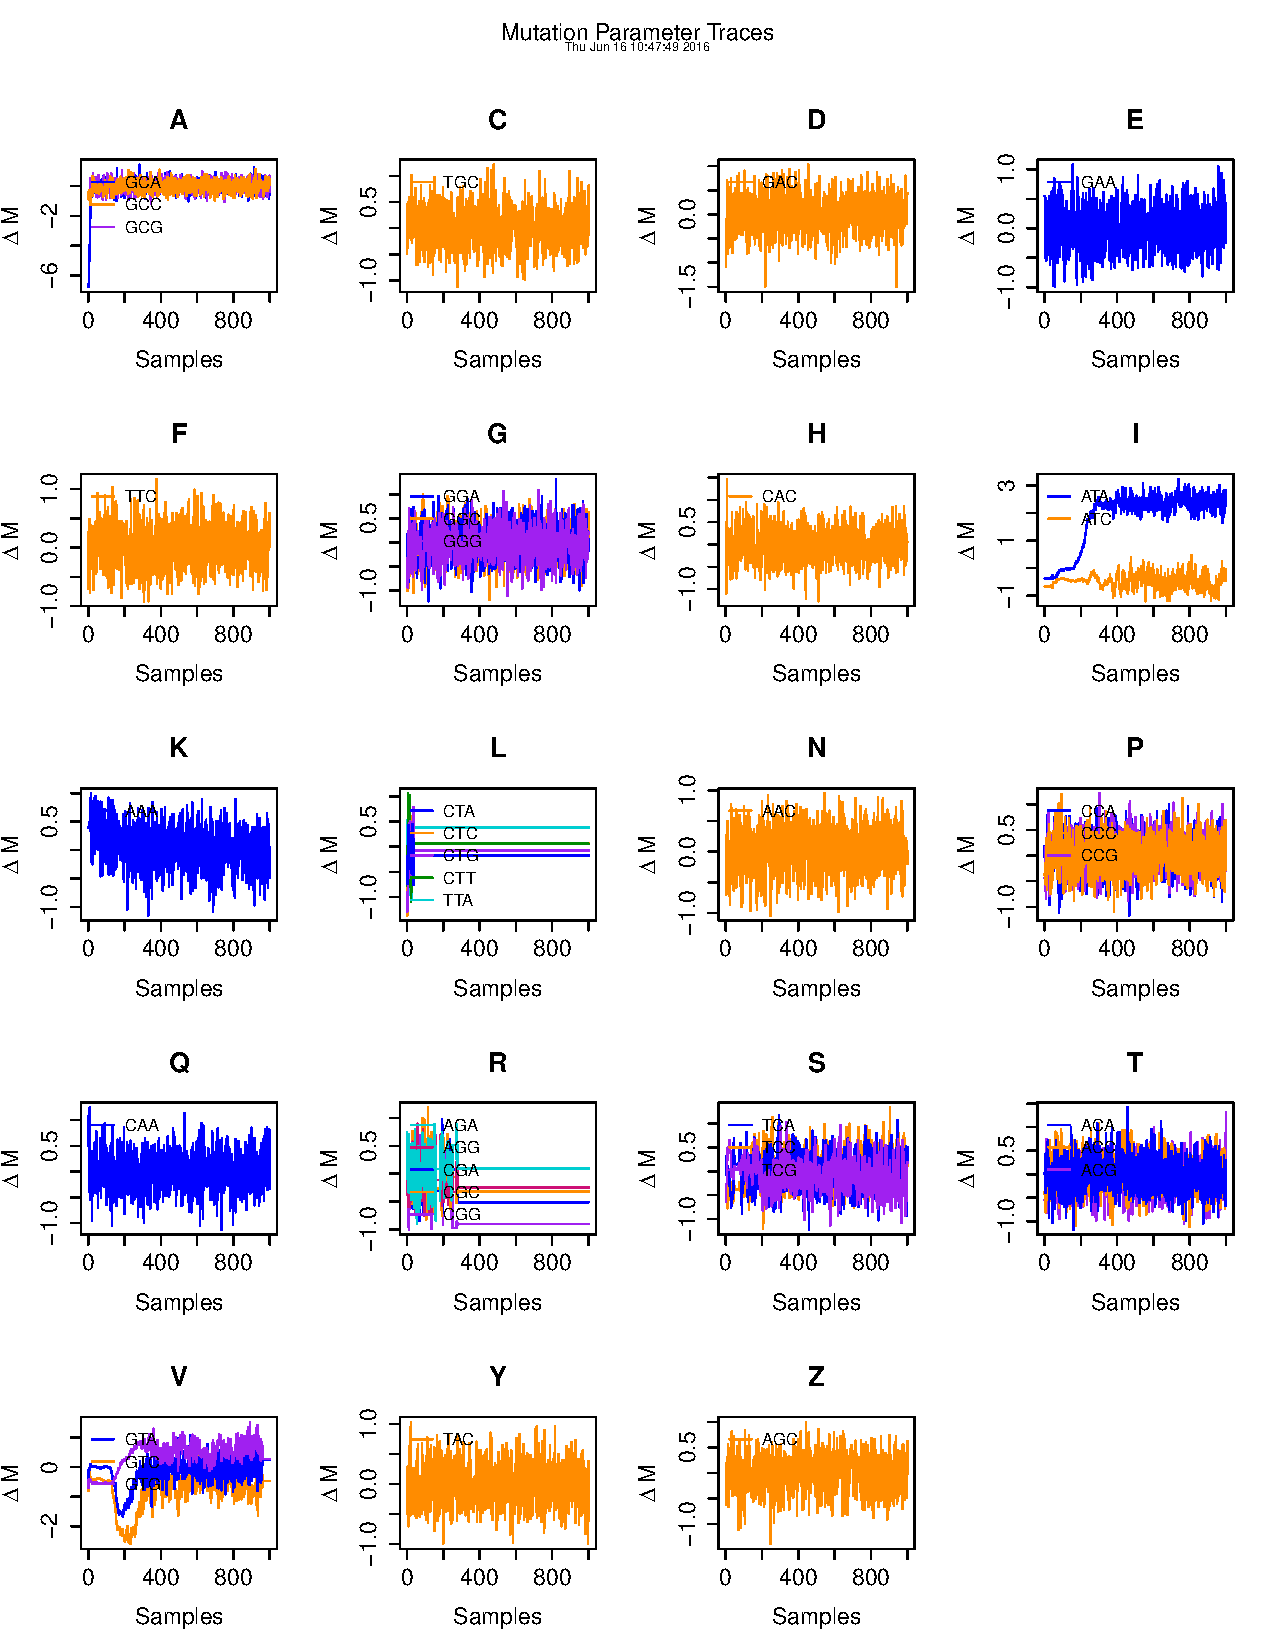
\includegraphics[scale=.65]{FONSE_Plots/2016/June_16/Run1_MutationTrace}
            \caption{Mutation Trace for Run 1}
            \label{fig:JUN16_MUT_R1}
        \end{figure}
        \begin{figure}
            \centering
            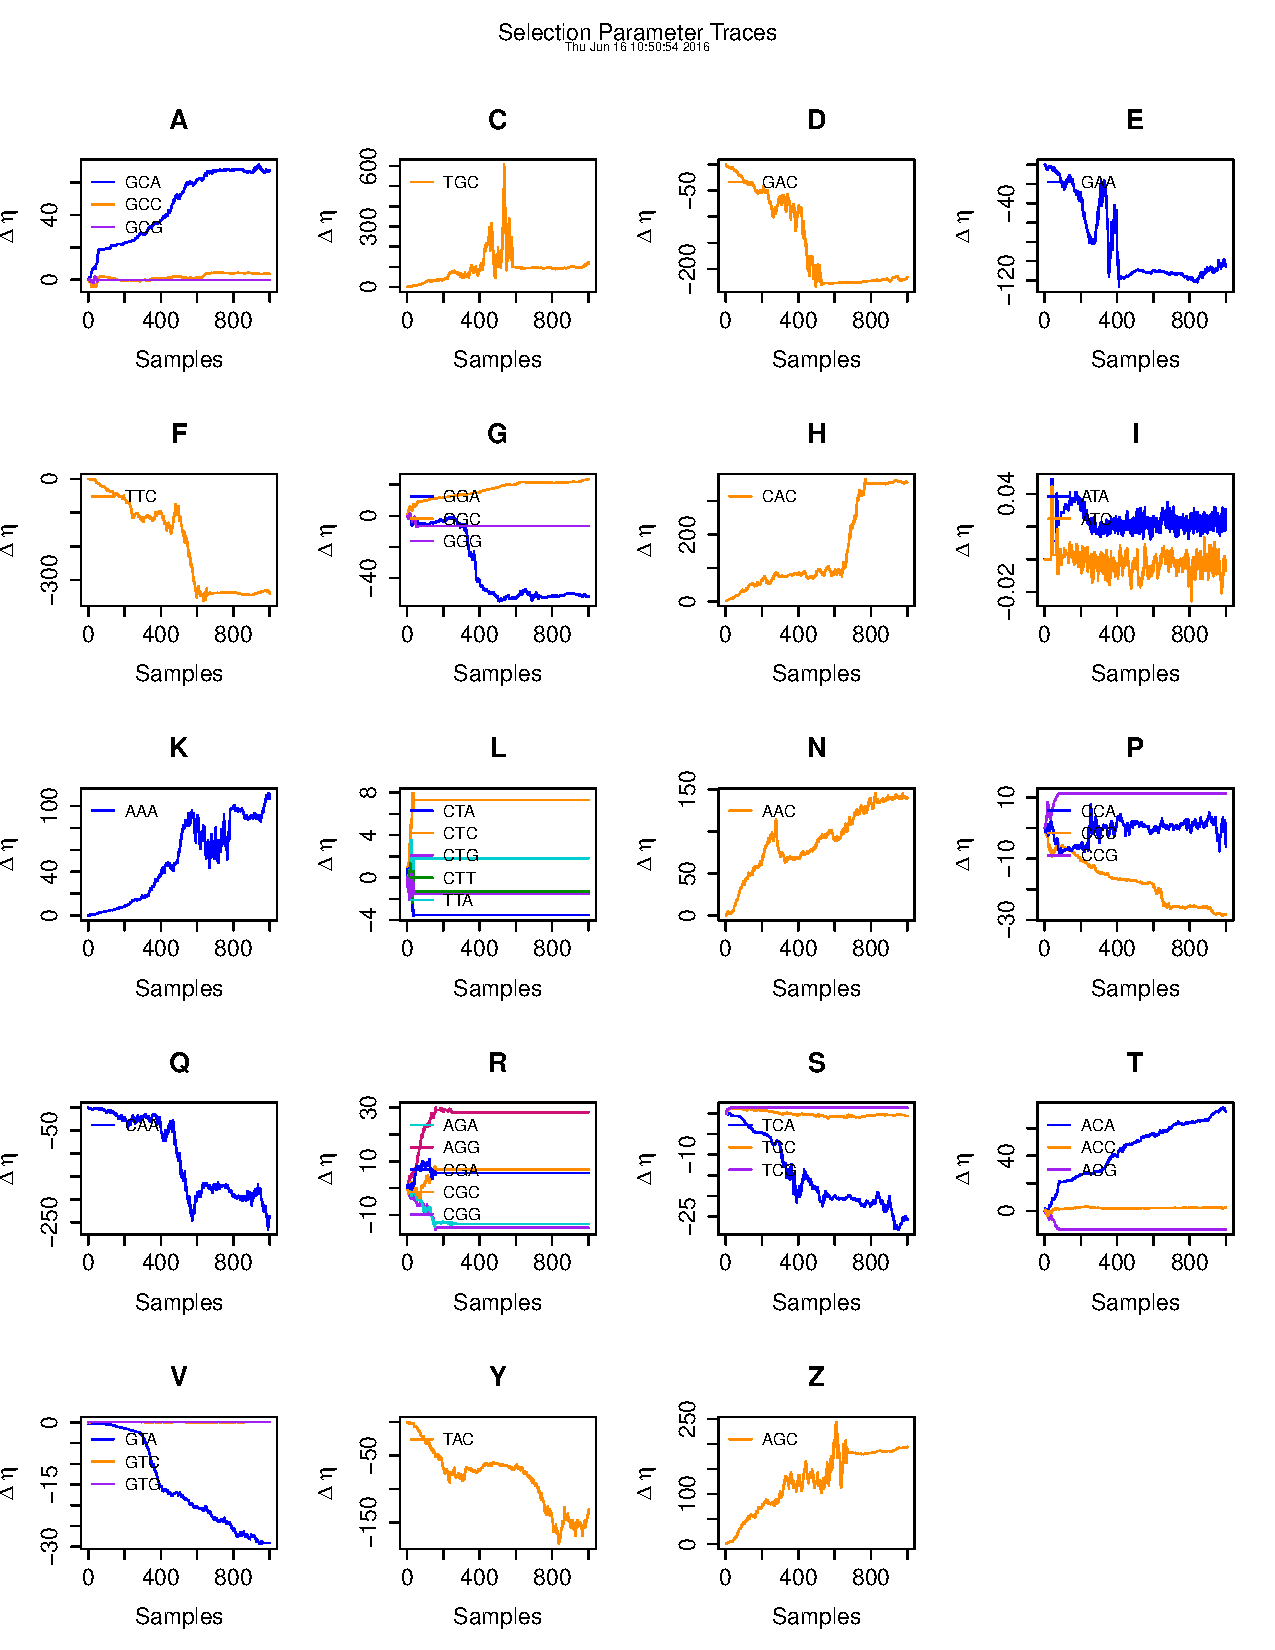
\includegraphics[scale=.65]{FONSE_Plots/2016/June_16/Run1_SelectionTrace}
            \caption{Selection Trace for Run 1}
            \label{fig:JUN16_SEL_R1}
        \end{figure}
        \begin{figure}
            \centering
            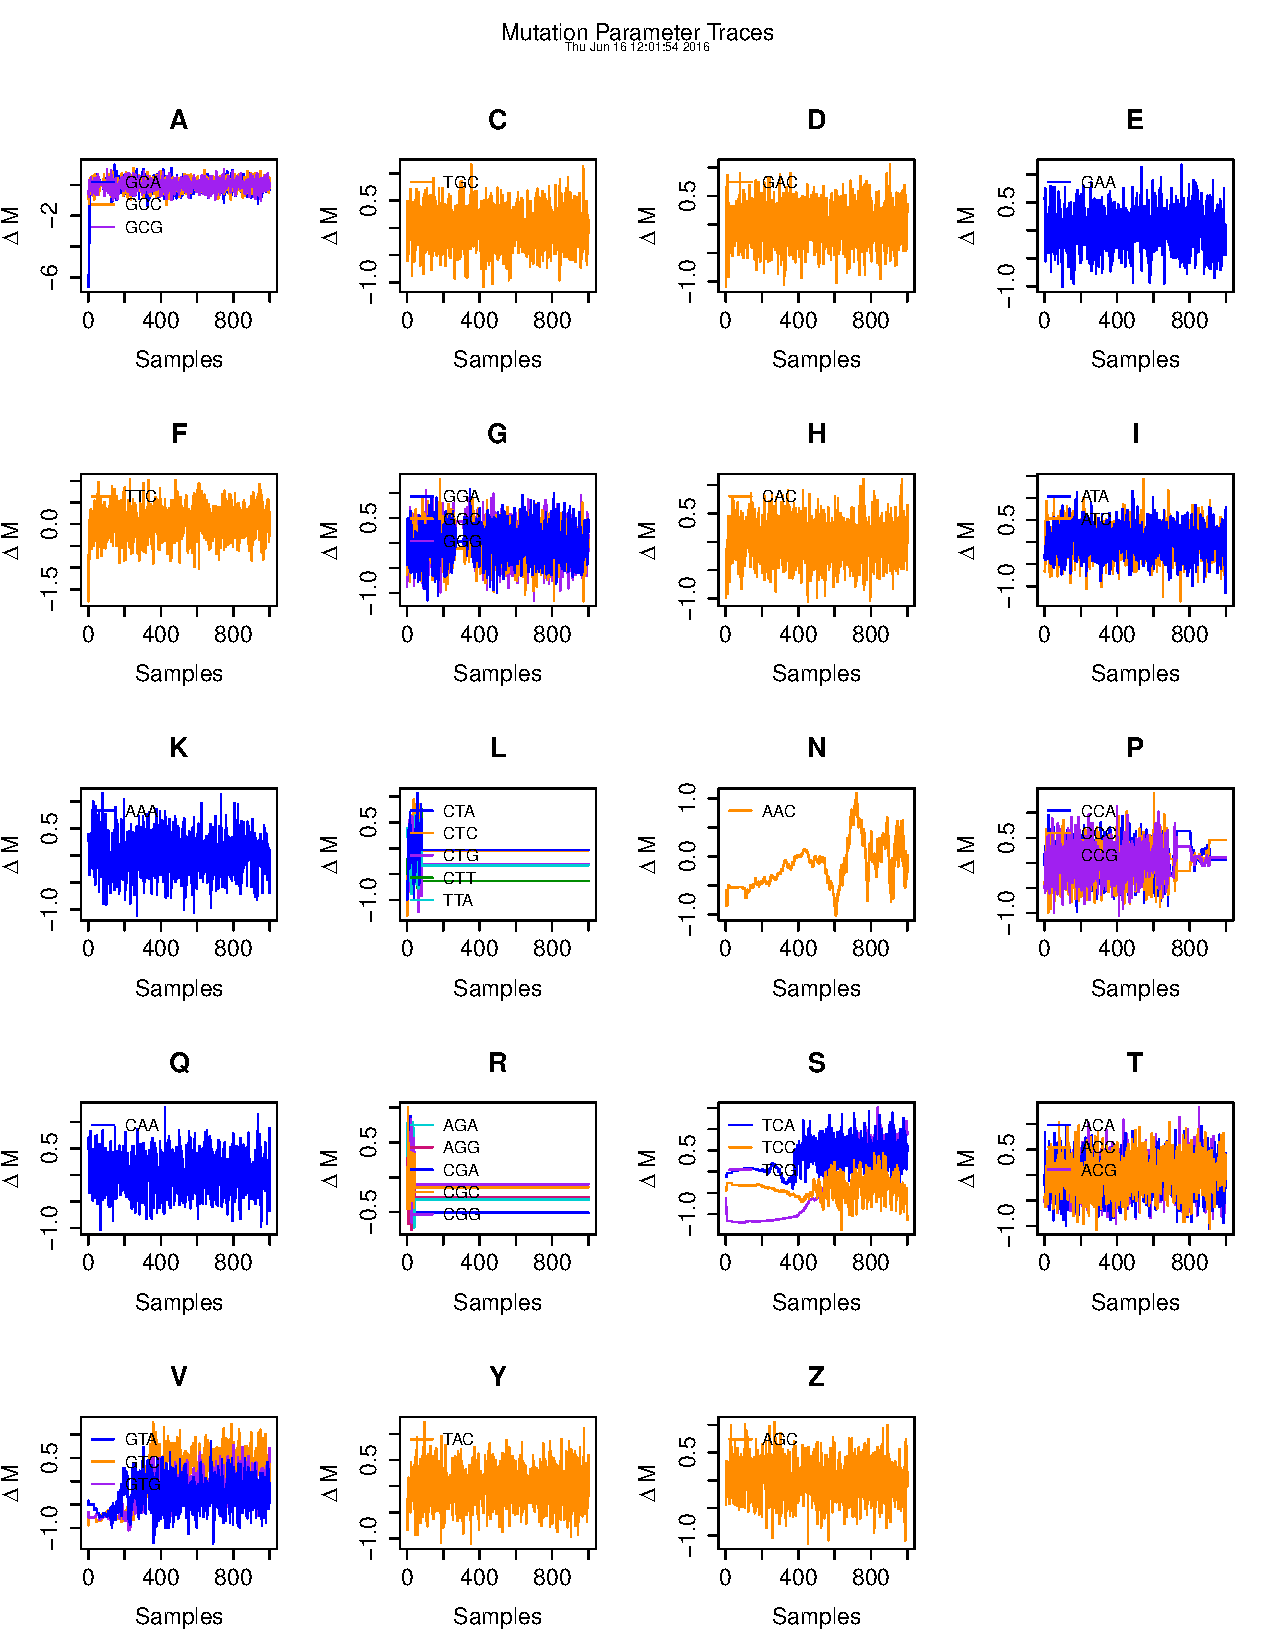
\includegraphics[scale=.65]{FONSE_Plots/2016/June_16/Run2_MutationTrace}
            \caption{Mutation Trace for Run 2}
            \label{fig:JUN16_MUT_R2}
        \end{figure}
         \begin{figure}
            \centering
            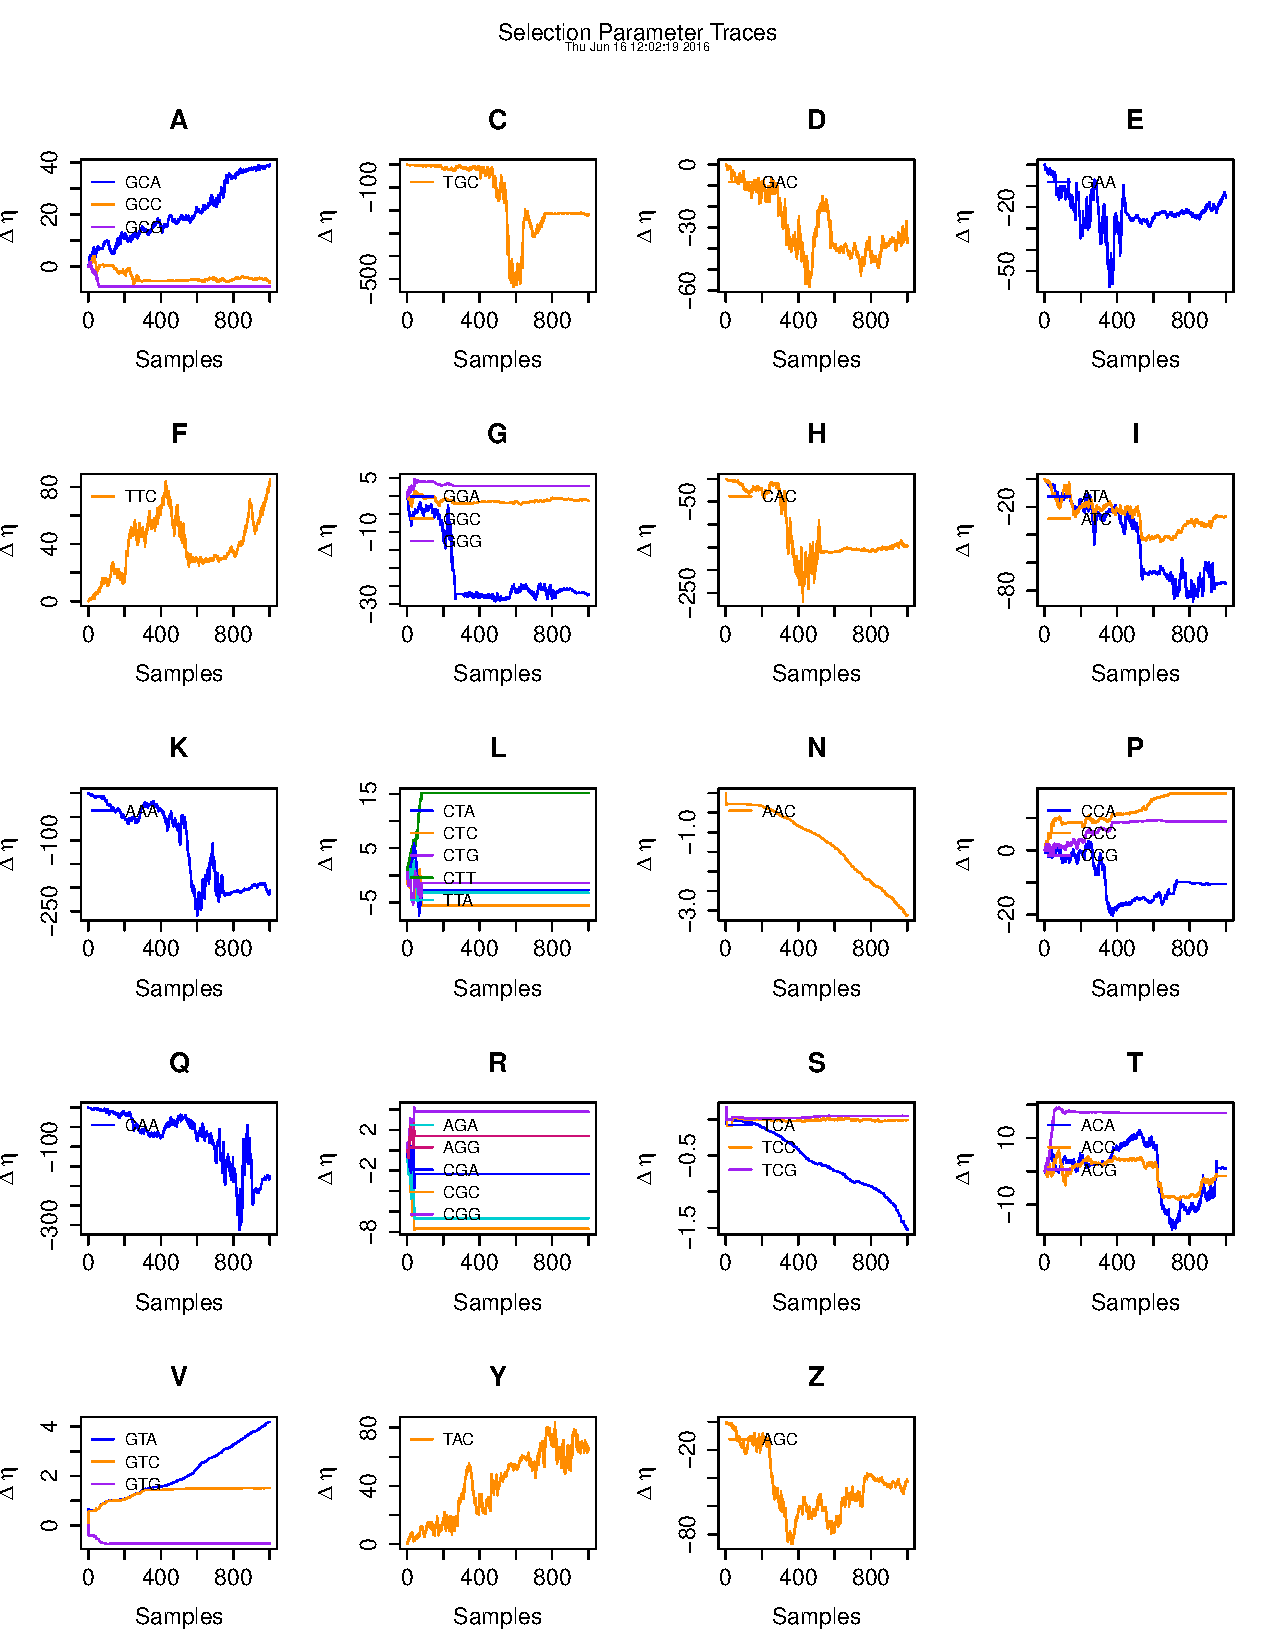
\includegraphics[scale=.65]{FONSE_Plots/2016/June_16/Run2_SelectionTrace}
            \caption{Selection Trace for Run 2}
            \label{fig:JUN16_SEL_R2}
        \end{figure}
        \begin{figure}
            \centering
            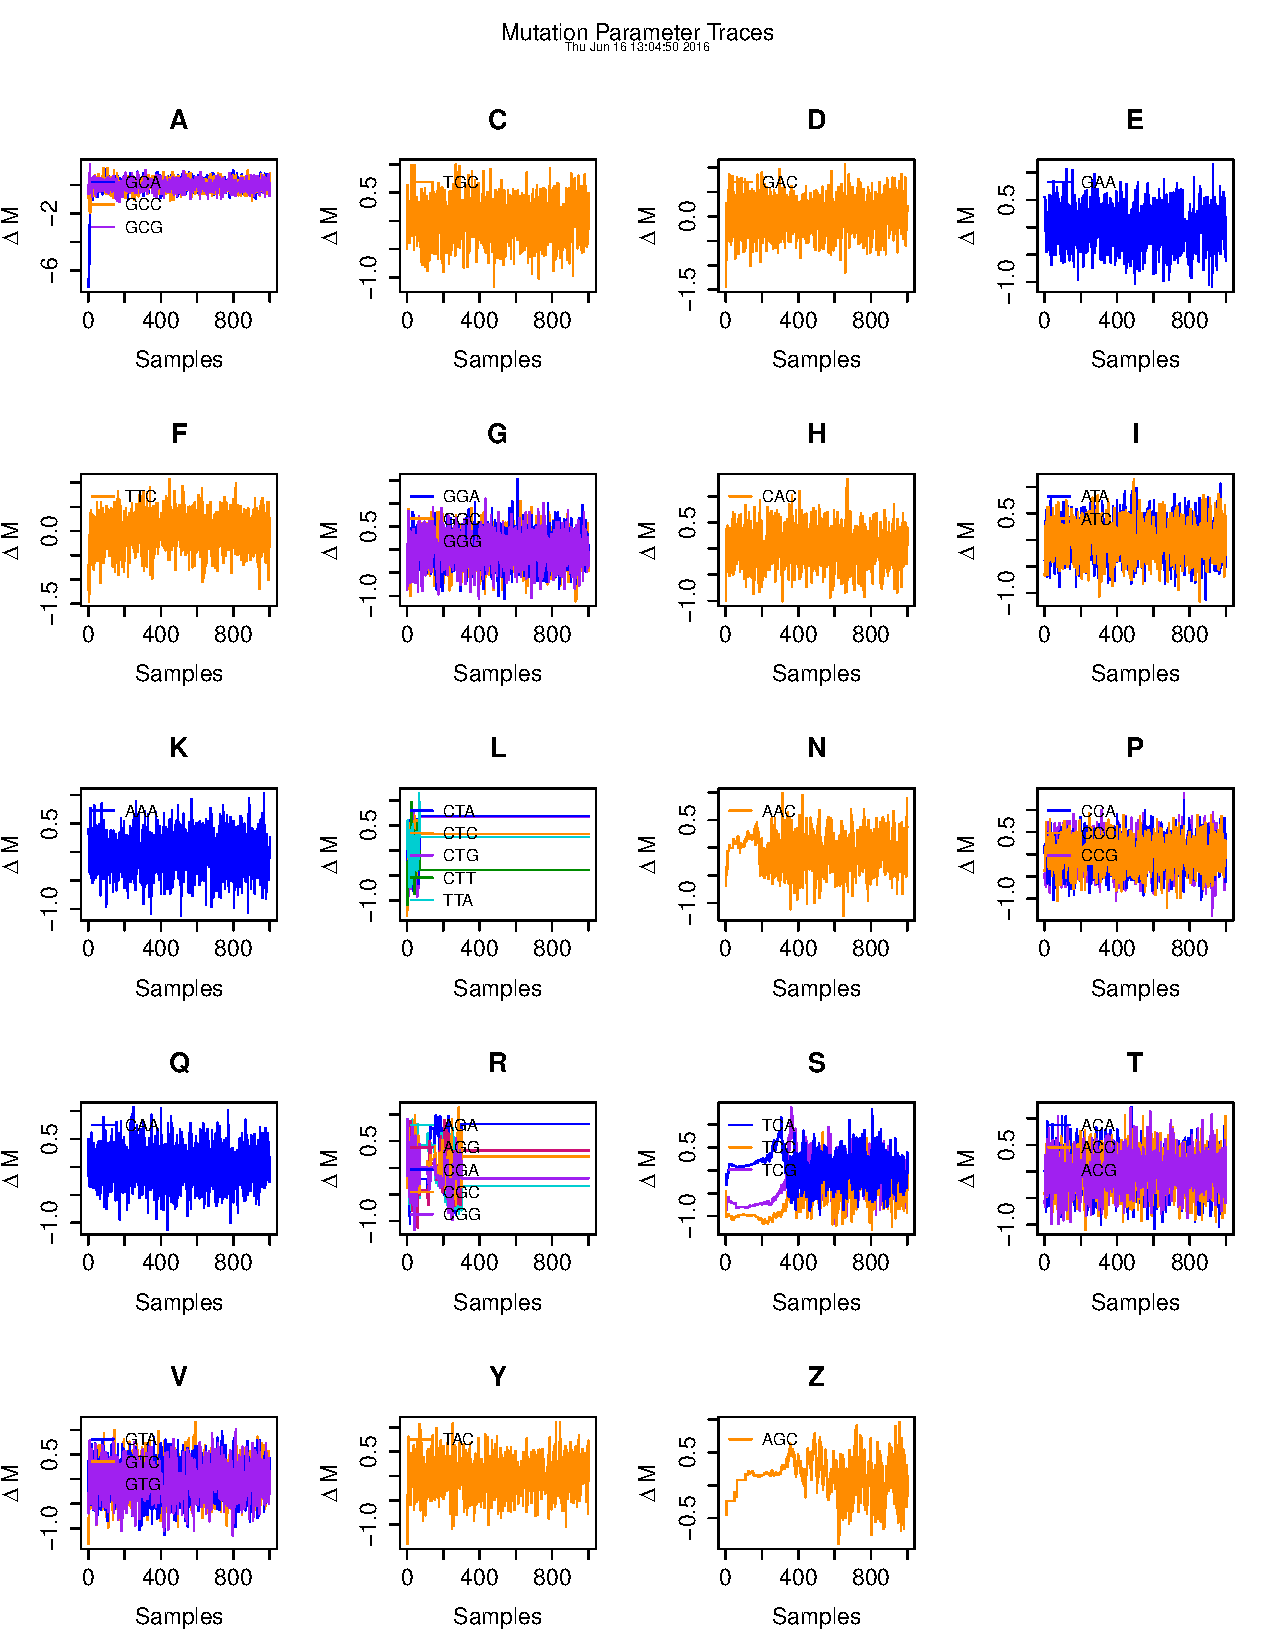
\includegraphics[scale=.65]{FONSE_Plots/2016/June_16/Run3_MutationTrace}
            \caption{Mutation Trace for Run 3}
            \label{fig:JUN16_MUT_R3}
        \end{figure}
        \begin{figure}
            \centering
            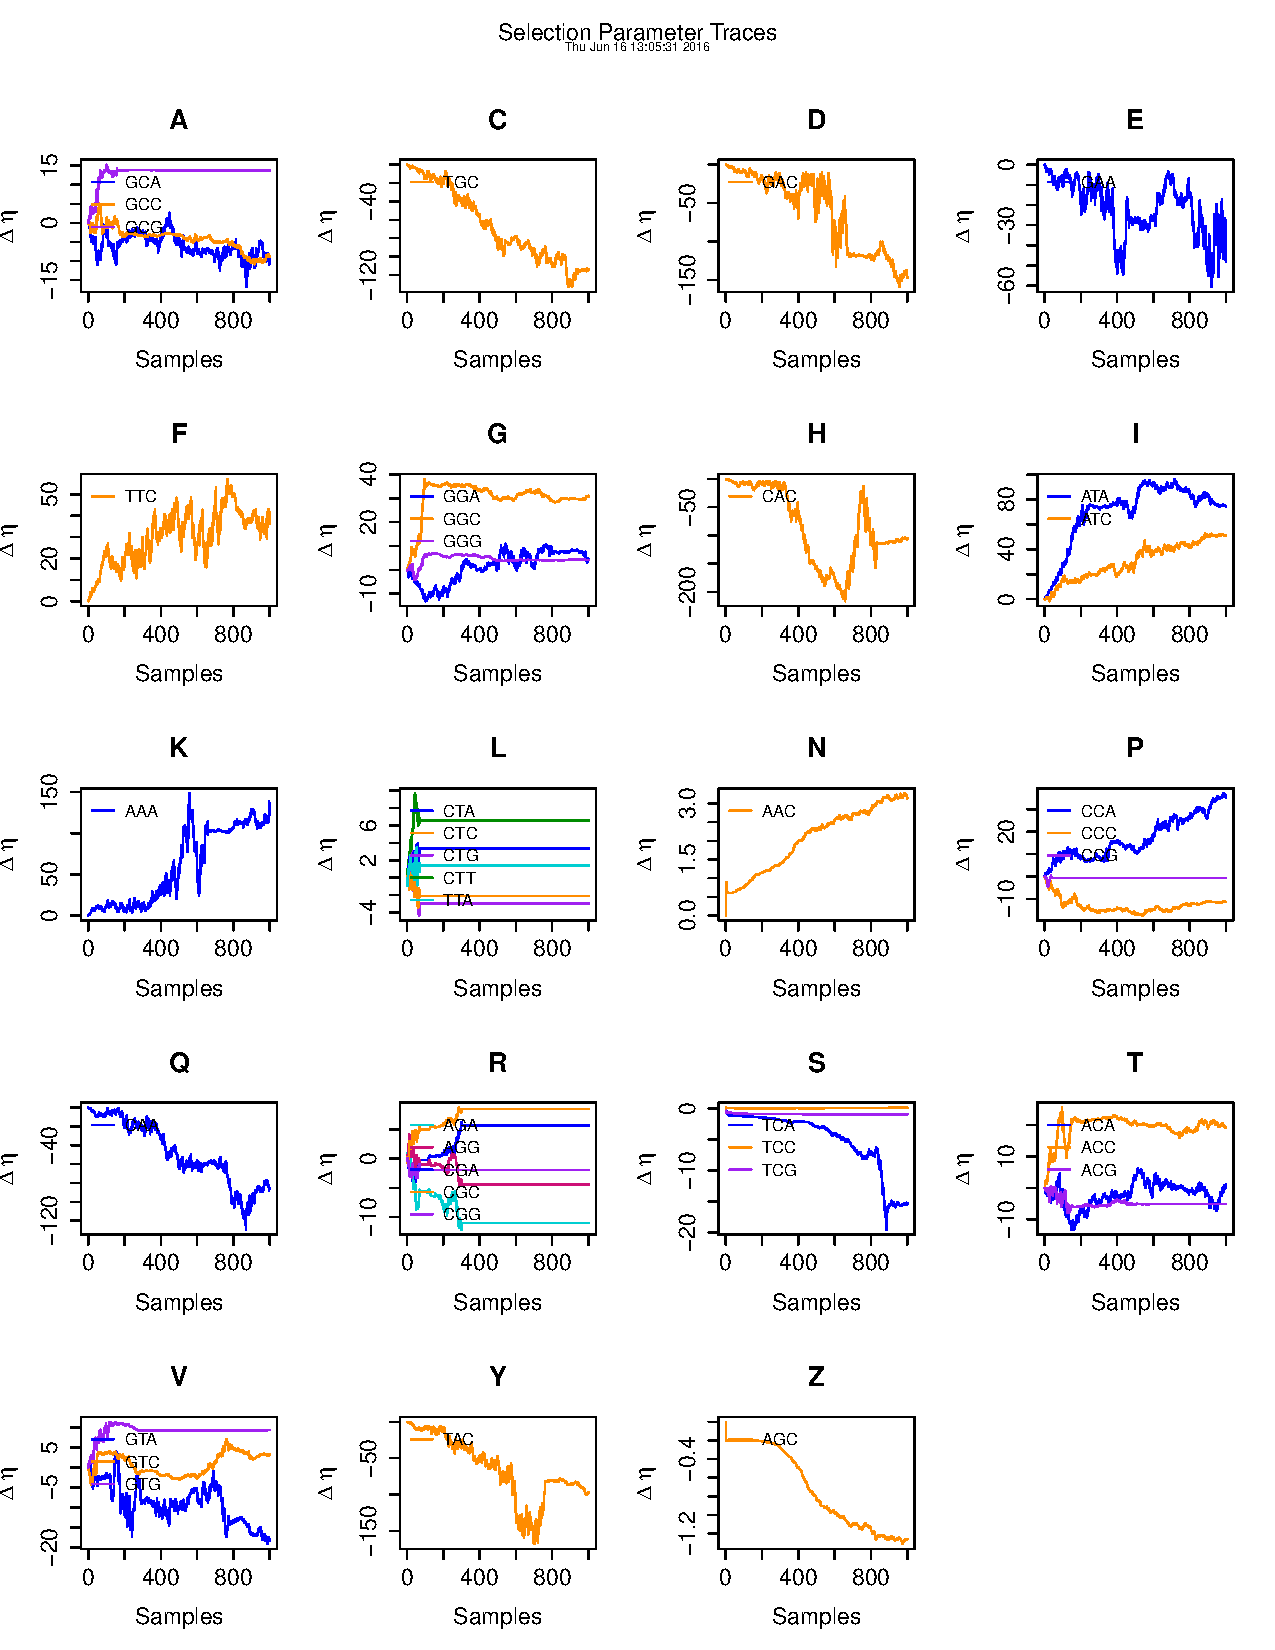
\includegraphics[scale=.65]{FONSE_Plots/2016/June_16/Run3_SelectionTrace}
            \caption{Selection Trace for Run 3}
            \label{fig:JUN16_SEL_R3}
        \end{figure}
    \end{itemize}
    
\labday{June 21, 2016}
    \begin{itemize}
        \item Most of today was spent resolving a problem with RStudio crashing. Both Cedric and I were experiencing this problem so we troubleshooted the issue and discovered that the issue was in a change that had been made in the R-only section of the code in Parameter.cpp. The issue was a "+1" had been added while referencing an element of an array, causing the program to attempt to reference out of the bounds of the array causing a segmentation fault. 
    \end{itemize}
\labday{June 22, 2016}
    \begin{itemize}
        \item Added documentation to the FONSE R-scripts from home due to illness.
    \end{itemize}
    
\labday{June 23, 2016}
    \begin{itemize}
        \item TODO: 
        \begin{itemize}
            \item Alter the code so that there is flexibility when someone invokes a prior i.e. specify whether or not a prior should be used.
            \item run the program with a uniform prior since it is proportional to no prior.
            \item Change from using a covariance matrix to the diagonal to see how that changes the issue where codons have acceptance rates of 0.
            \item Alternatively update the covariance matrix instead.
            \item Check to see if taking the mutation prior out of ROC causes the same phenomenon.
            \item Dump out the values of the genome step of MCMC so we can observe the traces per amino acid.
            \item Put in traces from when the code crashes into the lab notes.
        \end{itemize}
    \end{itemize}
    
\labday{June 24, 2016}
    \begin{itemize}
        \item As requested, I removed the prior from FONSE and ran the model twice in order to get more data and plots showing what's going wrong with the algorithm.
\footnote{mikeg: 06/24/16 -- 
  \begin{itemize}
  \item Is this all you were able to get done today?  If not, your notes should reflect this and, in general, be more detailed.
  \item What did the ROC runs show?  If you were unable to run it, why is this?
  \item Your choice of file names for plots is good and organizing them by date is also good. 
    However, you should also incorporate the year into your folder structure (e.g. Fig/2016/06/24).
  \item It appears that \DeltaEta also goes to unrealistic values, not just \DeltaM.
  \item Please add the $\sigma_\phi$ trace.
  \item There may be information in the earlier steps of the traces that we can't observe because the final plots cover such large ranges. 
    Please generate and add plots that focus in on the earlier steps.
    We want to know if the code behaves normally at any point or if it is always climbing downwards.
  \item Where are the traces for the individual AA per our discussion yesterday?
  \item As requested, please respond to my previous notes created using \textbackslash footnote\{\}.
    I'm particularly concerned with your inability to run things on newton.
  \end{itemize}
}
\footnote{aland: 06/27/16 --
    \begin{itemize}
        \item Documentation was done while FONSE was running
        \item I hadn't been able to run ROC at this time. Cedric has since helped me and I'm now able to do so.
        \item I'm still in the process of implementing the traces of individual AA's. Both that and including plots that focus on earlier steps are on my TODO list.
    \end{itemize}
}
    \item Run 1: b = 0.001, samples = 1000, thinning = 1.
        
    \begin{figure}
        \centering
        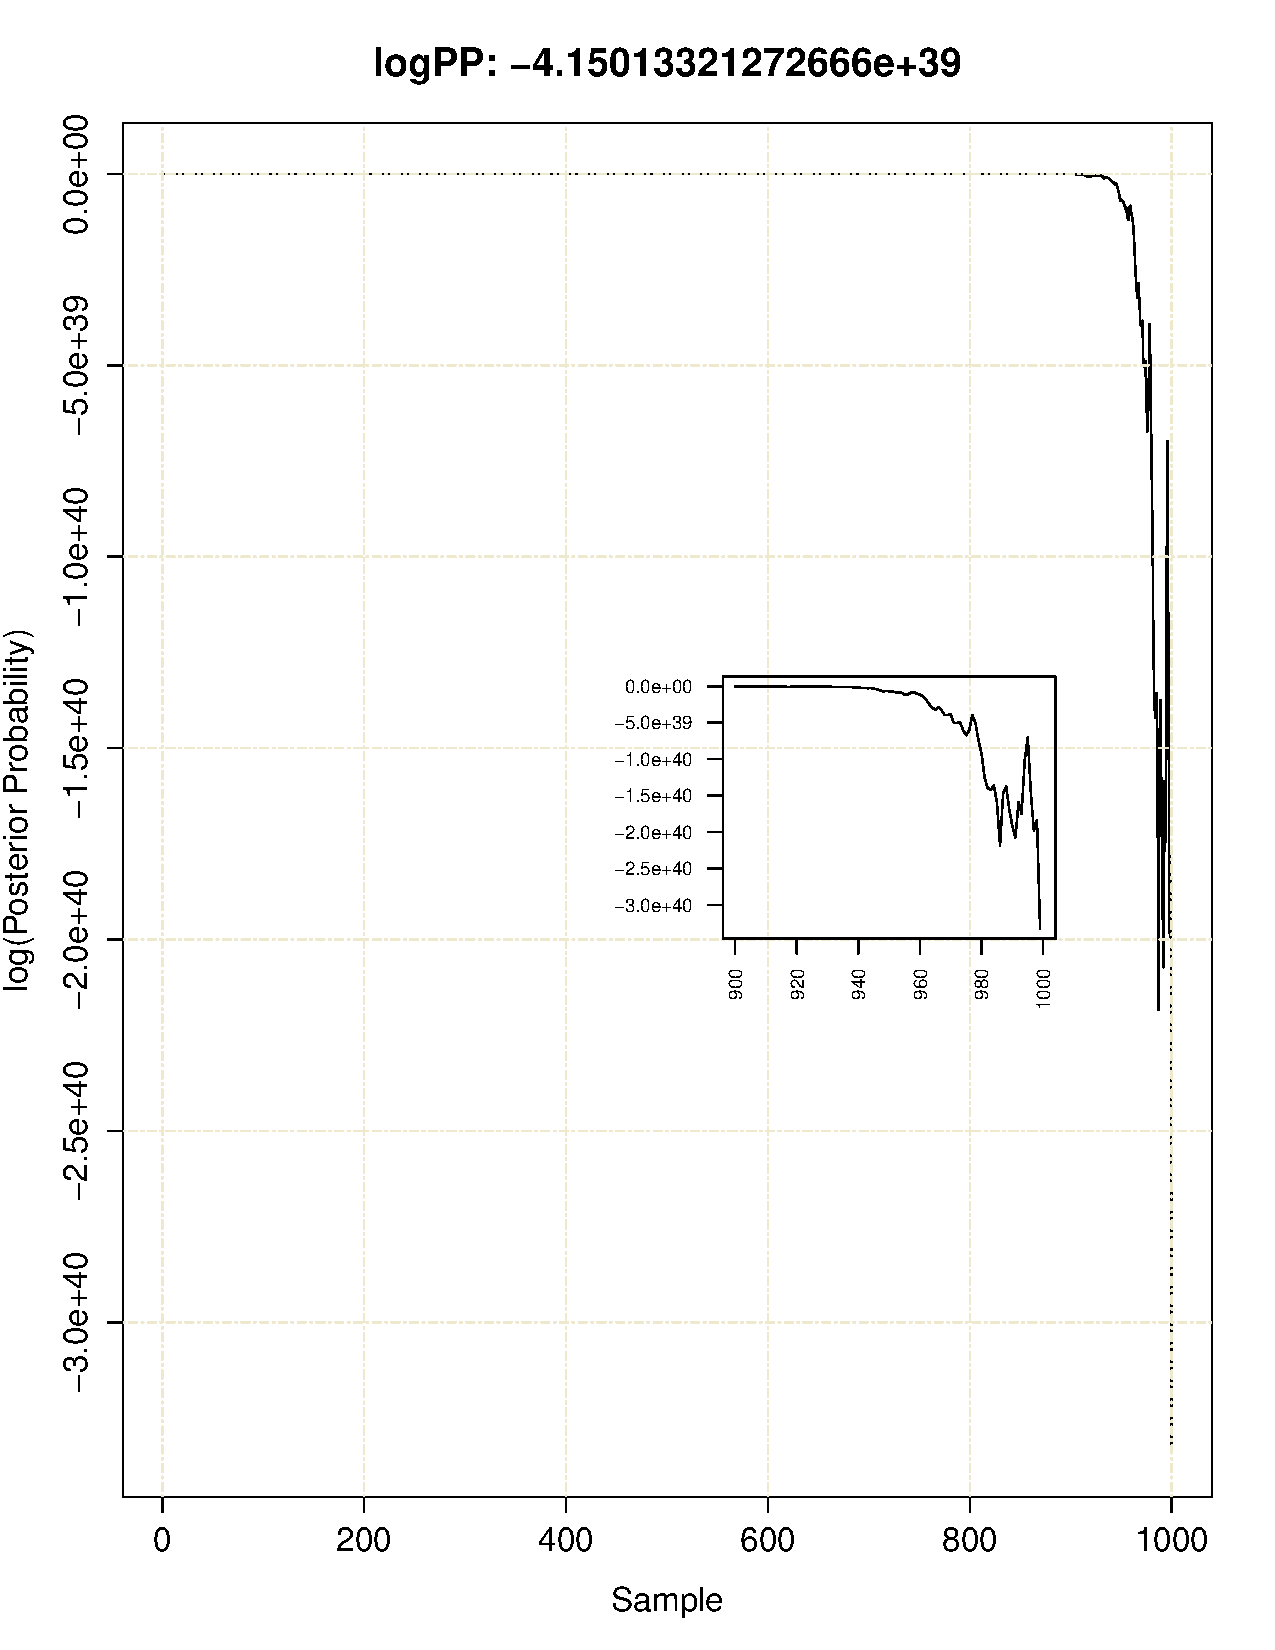
\includegraphics[scale=.65]{FONSE_Plots/2016/June_24/Run1_LogLikeTrace}
        \caption{LogLikelihood trace for Run 1}
        \label{fig:JUN24_LOG_R1}
    \end{figure}
    \begin{figure}
        \centering
        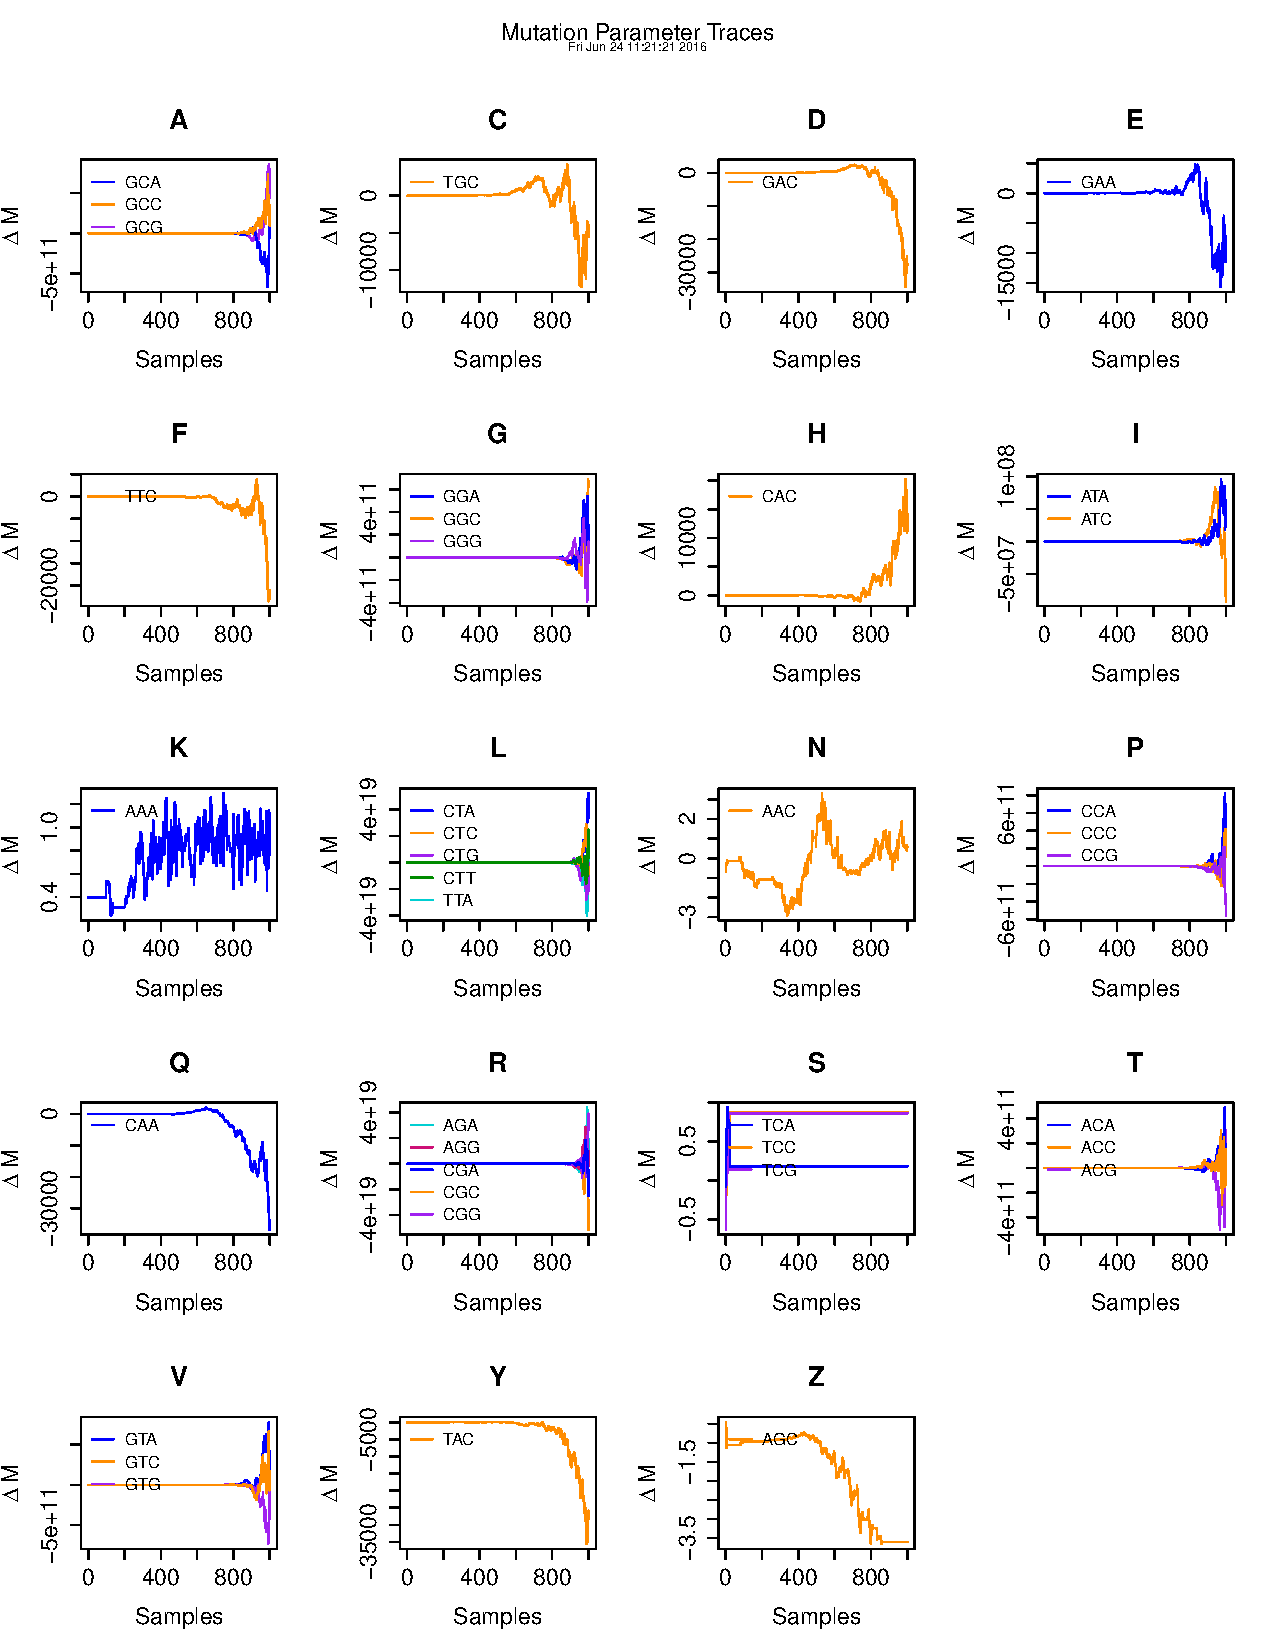
\includegraphics[scale=.65]{FONSE_Plots/2016/June_24/Run1_MutationTrace}
        \caption{Mutation trace for Run 1}
        \label{fig:JUN24_MUT_R1}
    \end{figure}
    \begin{figure}
        \centering
        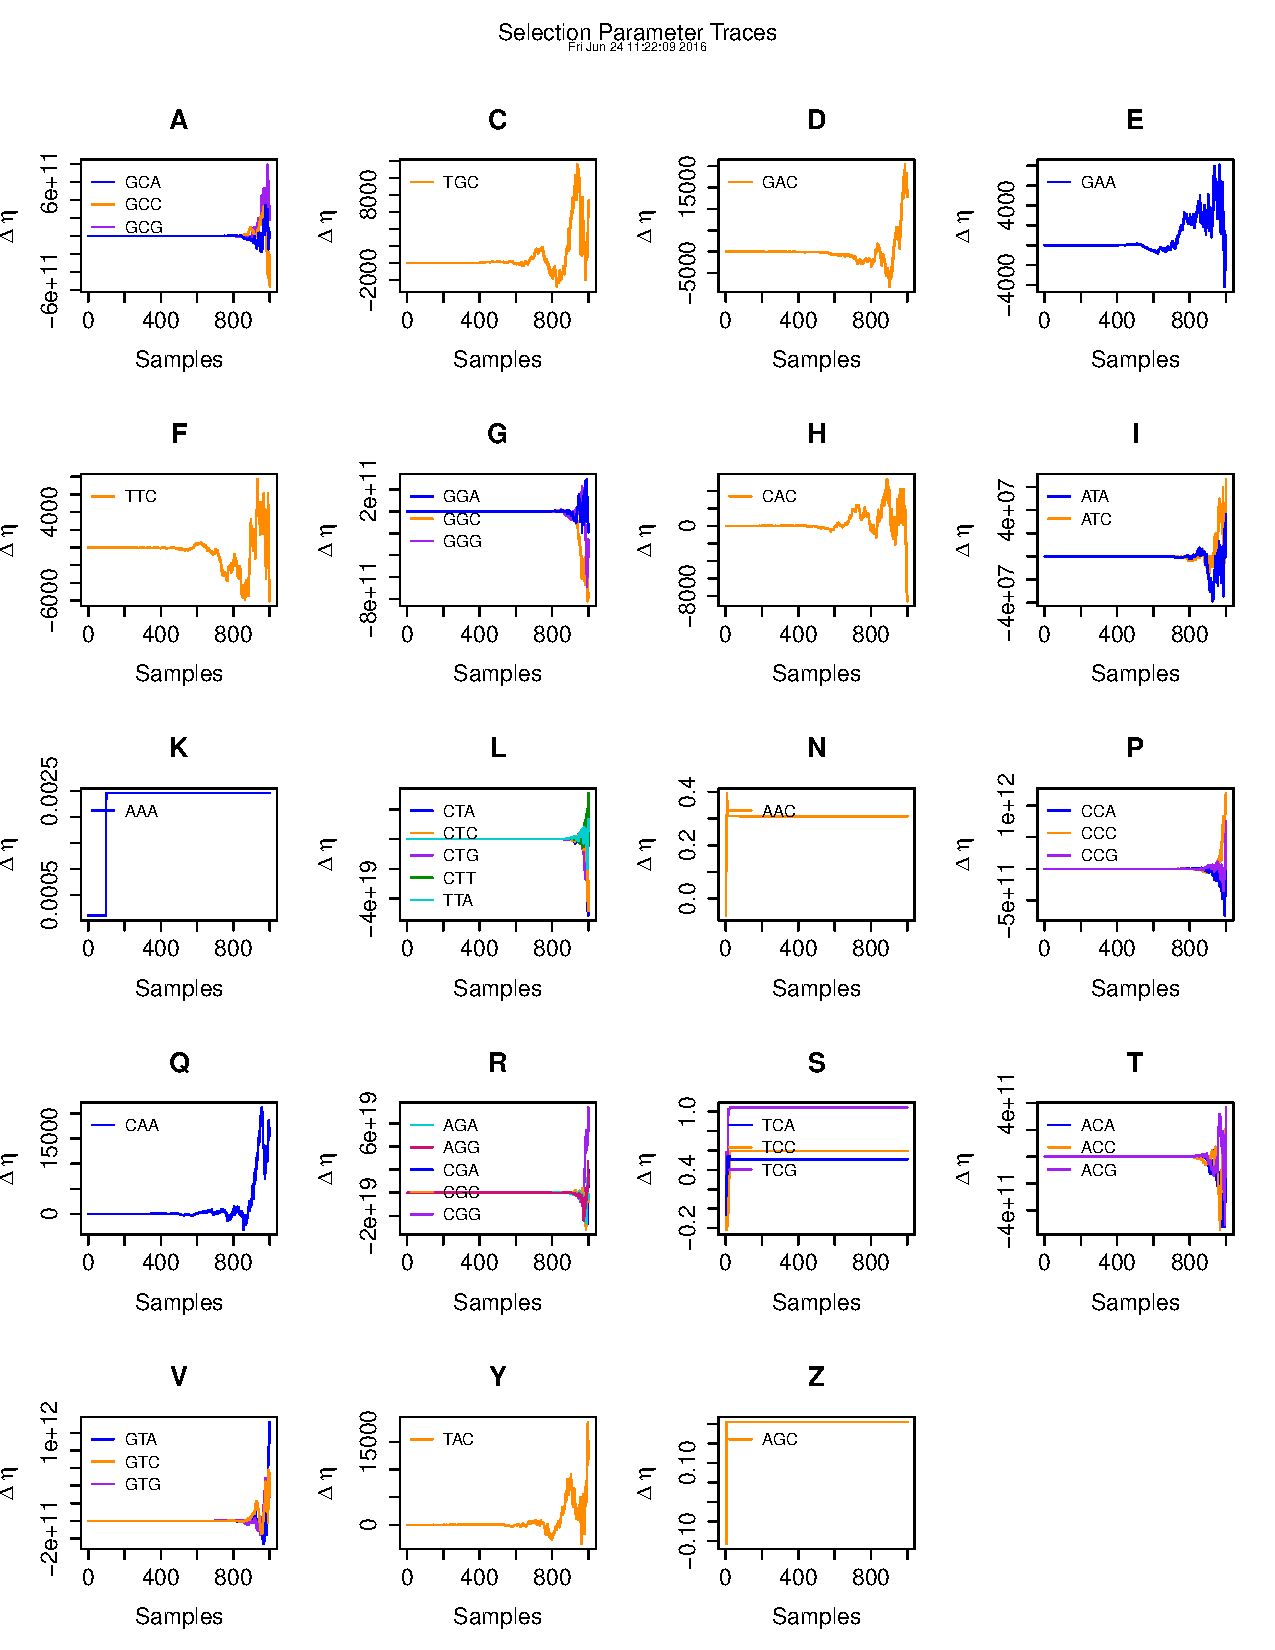
\includegraphics[scale=.65]{FONSE_Plots/2016/June_24/Run1_SelectionTrace}
        \caption{Selection trace for Run 1}
        \label{fig:JUN24_SEL_R1}
    \end{figure}
    \begin{figure}
        \centering
        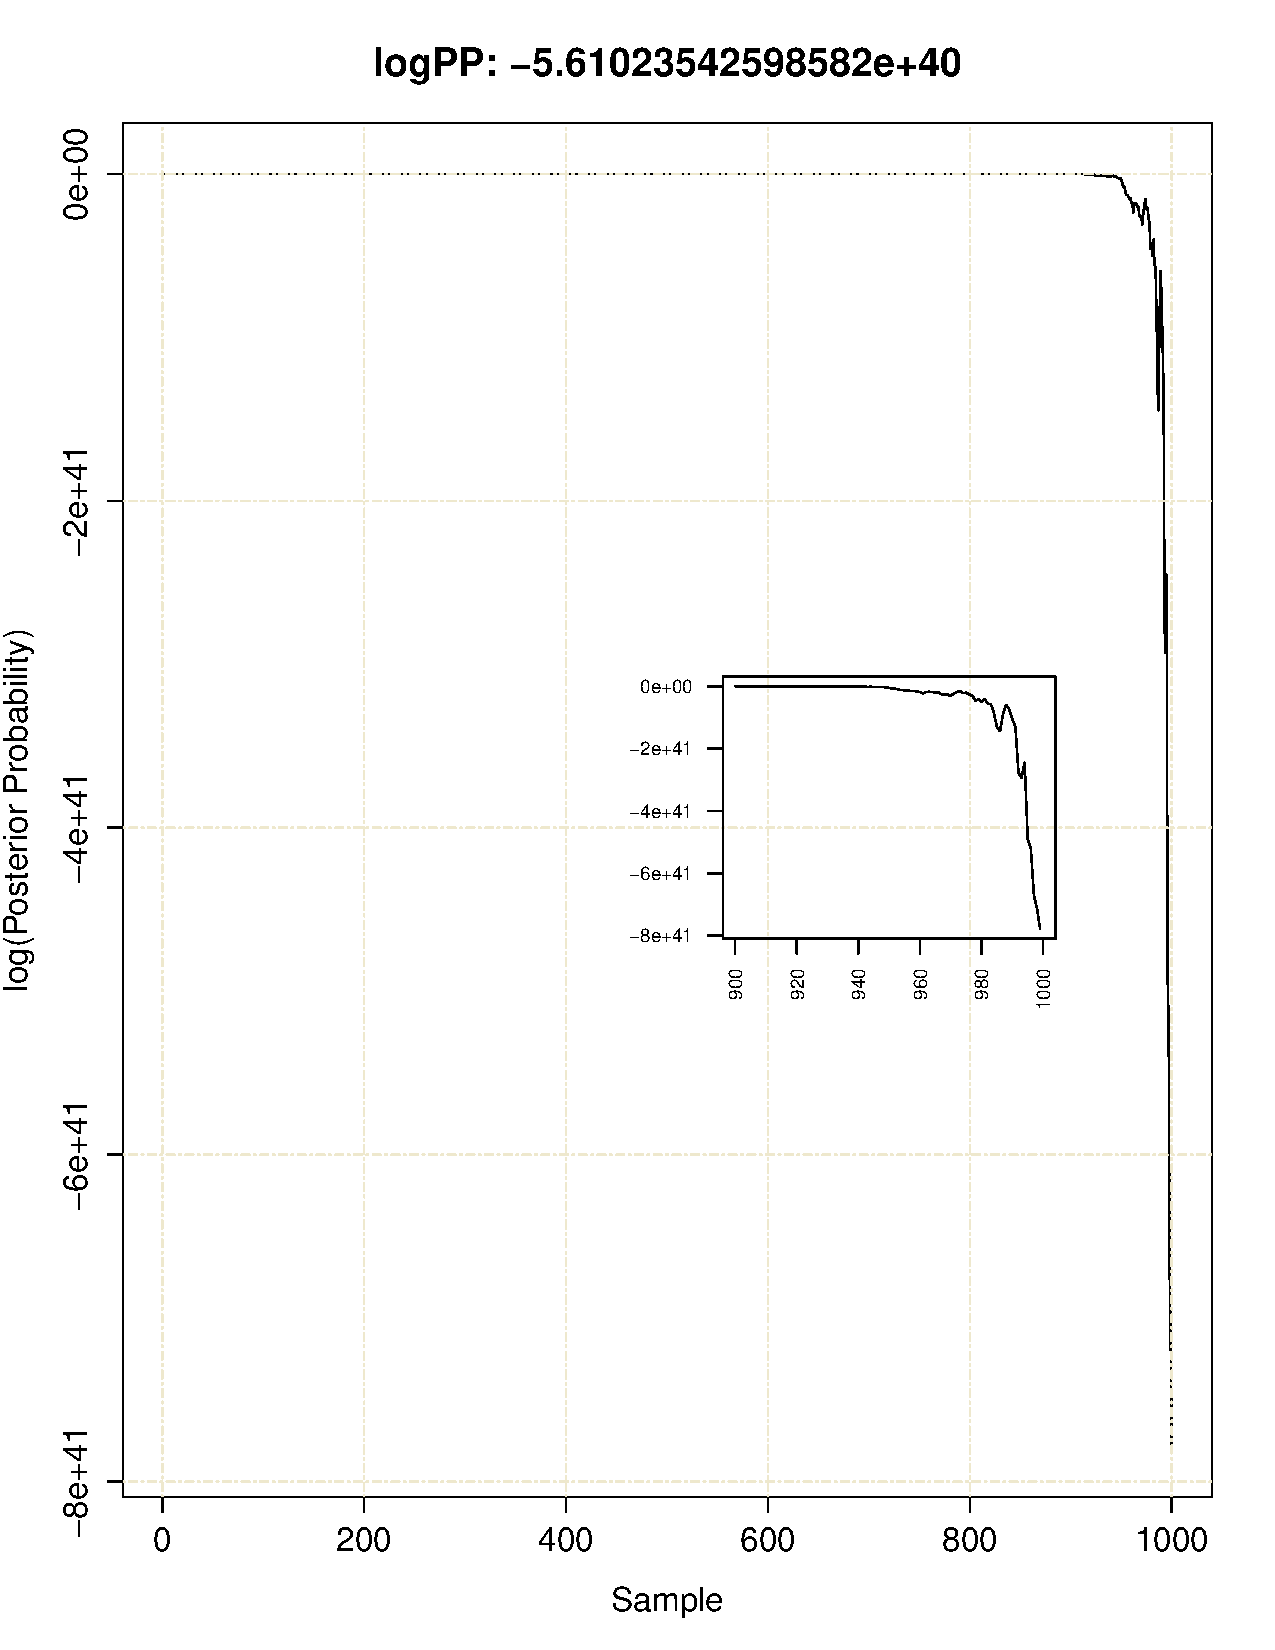
\includegraphics[scale=.65]{FONSE_Plots/2016/June_24/Run2_LogLikeTrace}
        \caption{LogLikelihood trace for Run 2}
        \label{fig:JUN24_LOG_R2}
    \end{figure}
    \begin{figure}
        \centering
        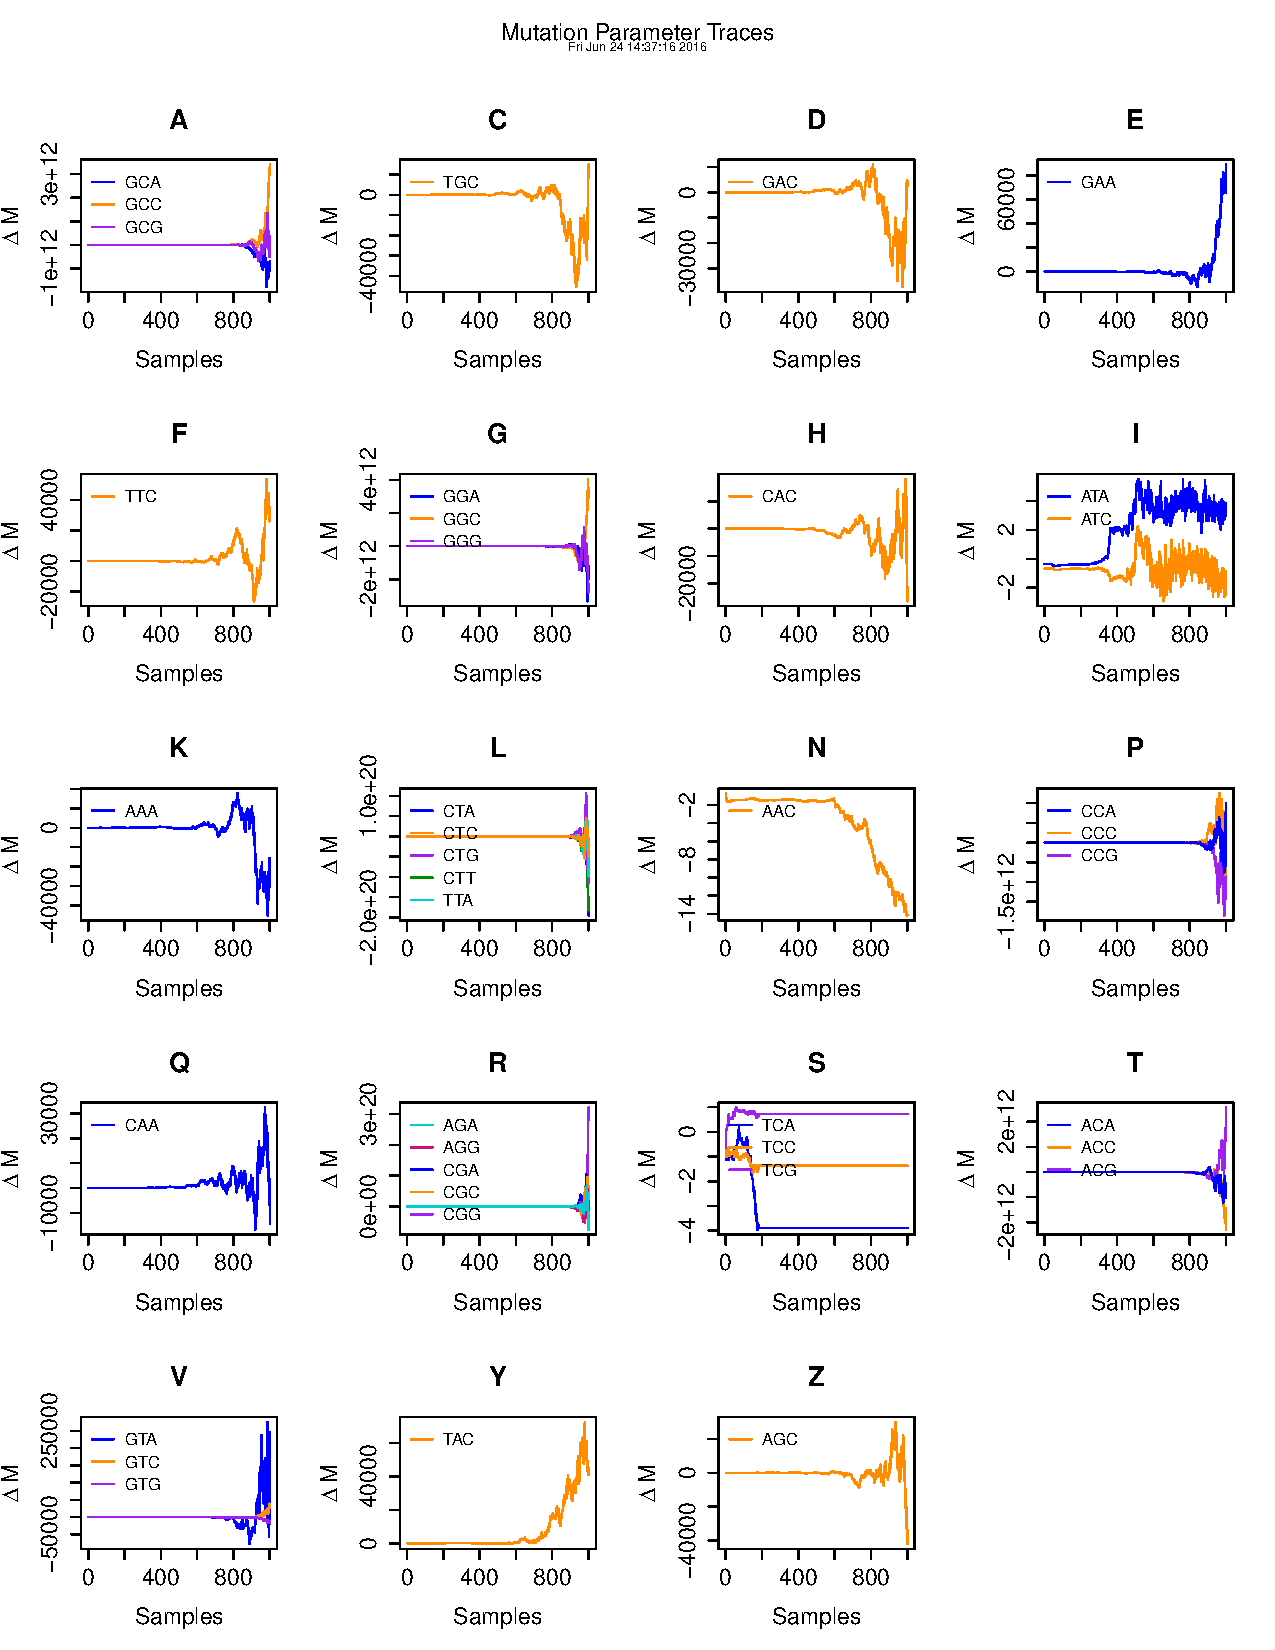
\includegraphics[scale=.65]{FONSE_Plots/2016/June_24/Run2_MutationTrace}
        \caption{Mutation trace for Run 2}
        \label{fig:JUN24_MUT_R2}
    \end{figure}
    \begin{figure}
        \centering
        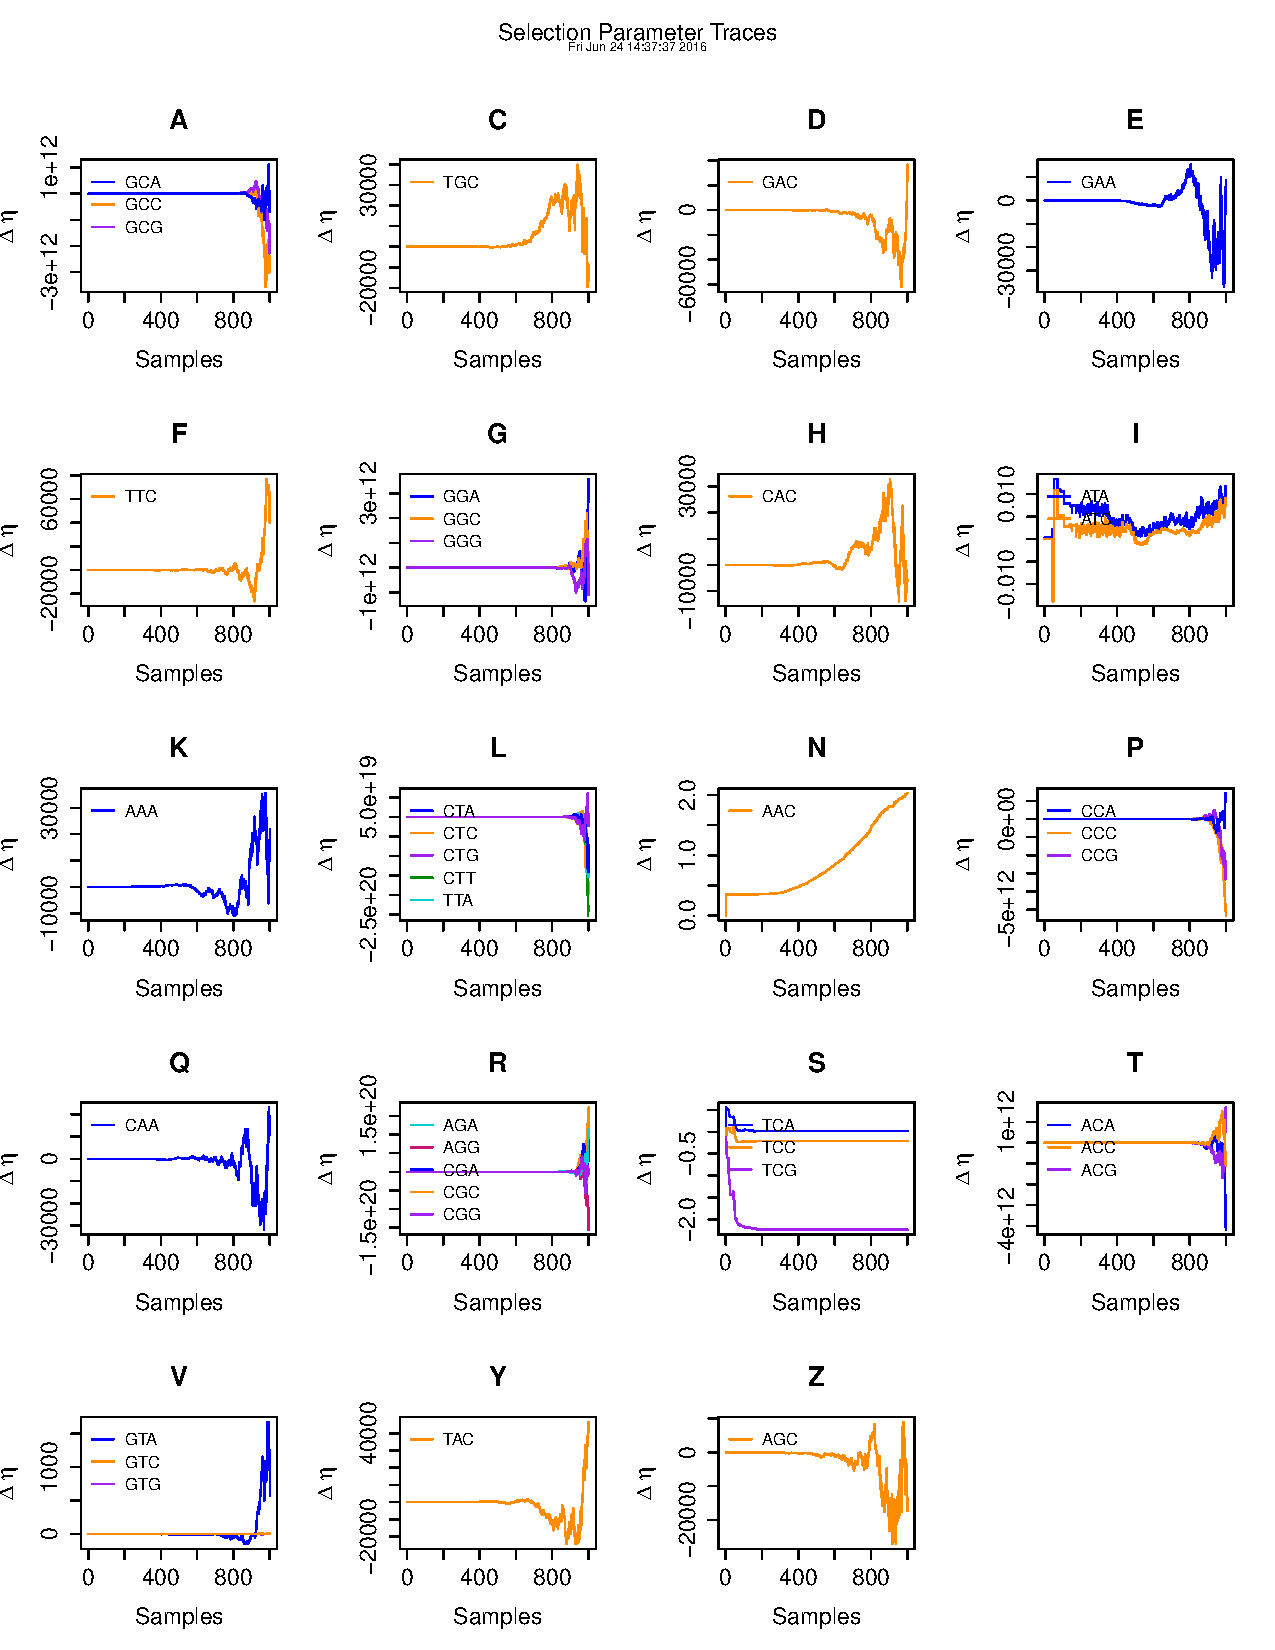
\includegraphics[scale=.65]{FONSE_Plots/2016/June_24/Run2_SelectionTrace}
        \caption{Selection trace for Run 2}
        \label{fig:JUN24_SEL_R2}
    \end{figure}
        
        \begin{itemize}
            \item Log Likelihood values plummet once again. At the end of the MCMC loop the value had reached -1.8e-40. See Figure \ref{fig:JUN24_LOG_R1}.\footnote{mikeg: 06/24/16 -- You should use the \textbackslash label\{\} and \textbackslash ref\{\} commands rather than labeling and referring to figures using hard coded numbers.}
            \item Acceptance rates for most of the codons were highly suspect with most having acceptance rates of 1 and others having rates of 0.
            \item Both mutation and selection traces seem consistent with the behavior of the other plots and parameters. See Figures \ref{fig:JUN24_MUT_R1} and \ref{fig:JUN24_SEL_R1}.
        \end{itemize}
        \item Run 2: b = 0.001, samples = 1000, thinning = 10. 
          \footnote{mikeg: 06/24/16 -- instead of cutting and pasting the exact same text, you should clearly state what you want to reader to infer from this second set.
          That is, ``the choice of thinning does not affect the model's behavior.''
        I would not have expected it to and, instead, would have recommended you do a run with a different $b$ value.}
        \begin{itemize}
            \item Log Likelihood values plummet once again. At the end of the MCMC loop the value had reached -7.1e-41. See Figure \ref{fig:JUN24_LOG_R2}.
            \item Acceptance rates for most of the codons were agian highly suspect with most having acceptance rates of 1 and others having rates of 0.
            \item Both mutation and selection traces again seem consistent with the behavior of the other plots and parameters. See Figures \ref{fig:JUN24_MUT_R2} and \ref{fig:JUN24_SEL_R2}.
        \end{itemize}
    \end{itemize}

\labday{June 27, 2016}
    \begin{itemize}
        \item Worked on the implementation of adding plots of the earlier stages of the trace for the log likelihood.
        \item Worked on altering the .SGE scripts so I can run them on Newton
        \item Added further documentation to FONSE.\footnote{Please be more informative on what aspects of the documentation you worked on.}
        \item Ran FONSE and ROC both without the prior, both with samples = 1000 and thinning = 10.
        \item FONSE: b = 0.001
        \begin{itemize}
            \item Log likelihood values plummeted once again, this time ending at -3.31e+41.
            \item High acceptance rates for most of the AA's with over half of them being 1. Those that weren't high or 1 were 0.
        \end{itemize}
        \item ROC with simulated data:
        \begin{itemize}
            \item Log likelihood values quickly rose and settled around -810000
            \item Very low acceptance rates for almost all AA's (some being moderate at around .35) with almost half being 0.
        \end{itemize}
    \end{itemize}
    
    \begin{figure}
        \centering
        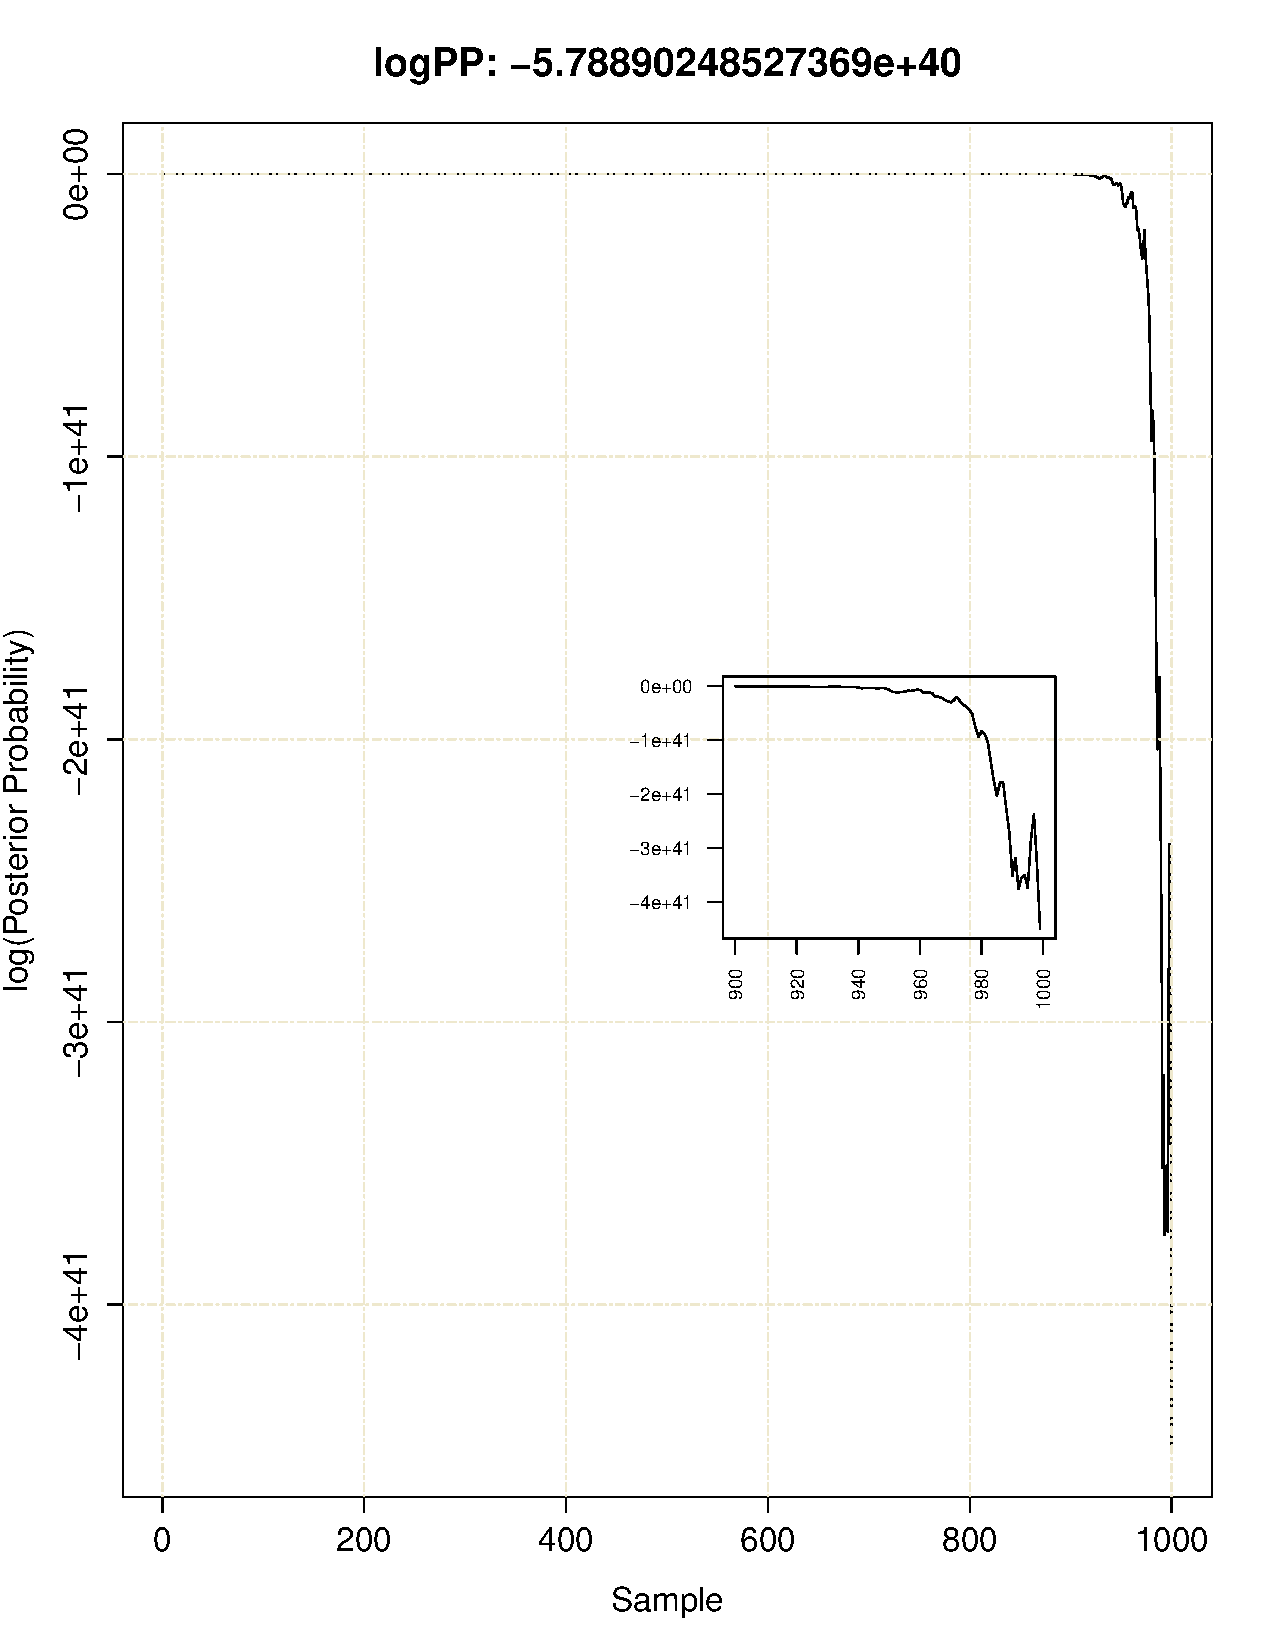
\includegraphics[scale=.65]{FONSE_Plots/2016/June_27/Run1_LogLikeTrace}
        \caption{LogLikelihood trace for FONSE}
        \label{fig:JUN27_FLOG}
    \end{figure}
    \begin{figure}
        \centering
        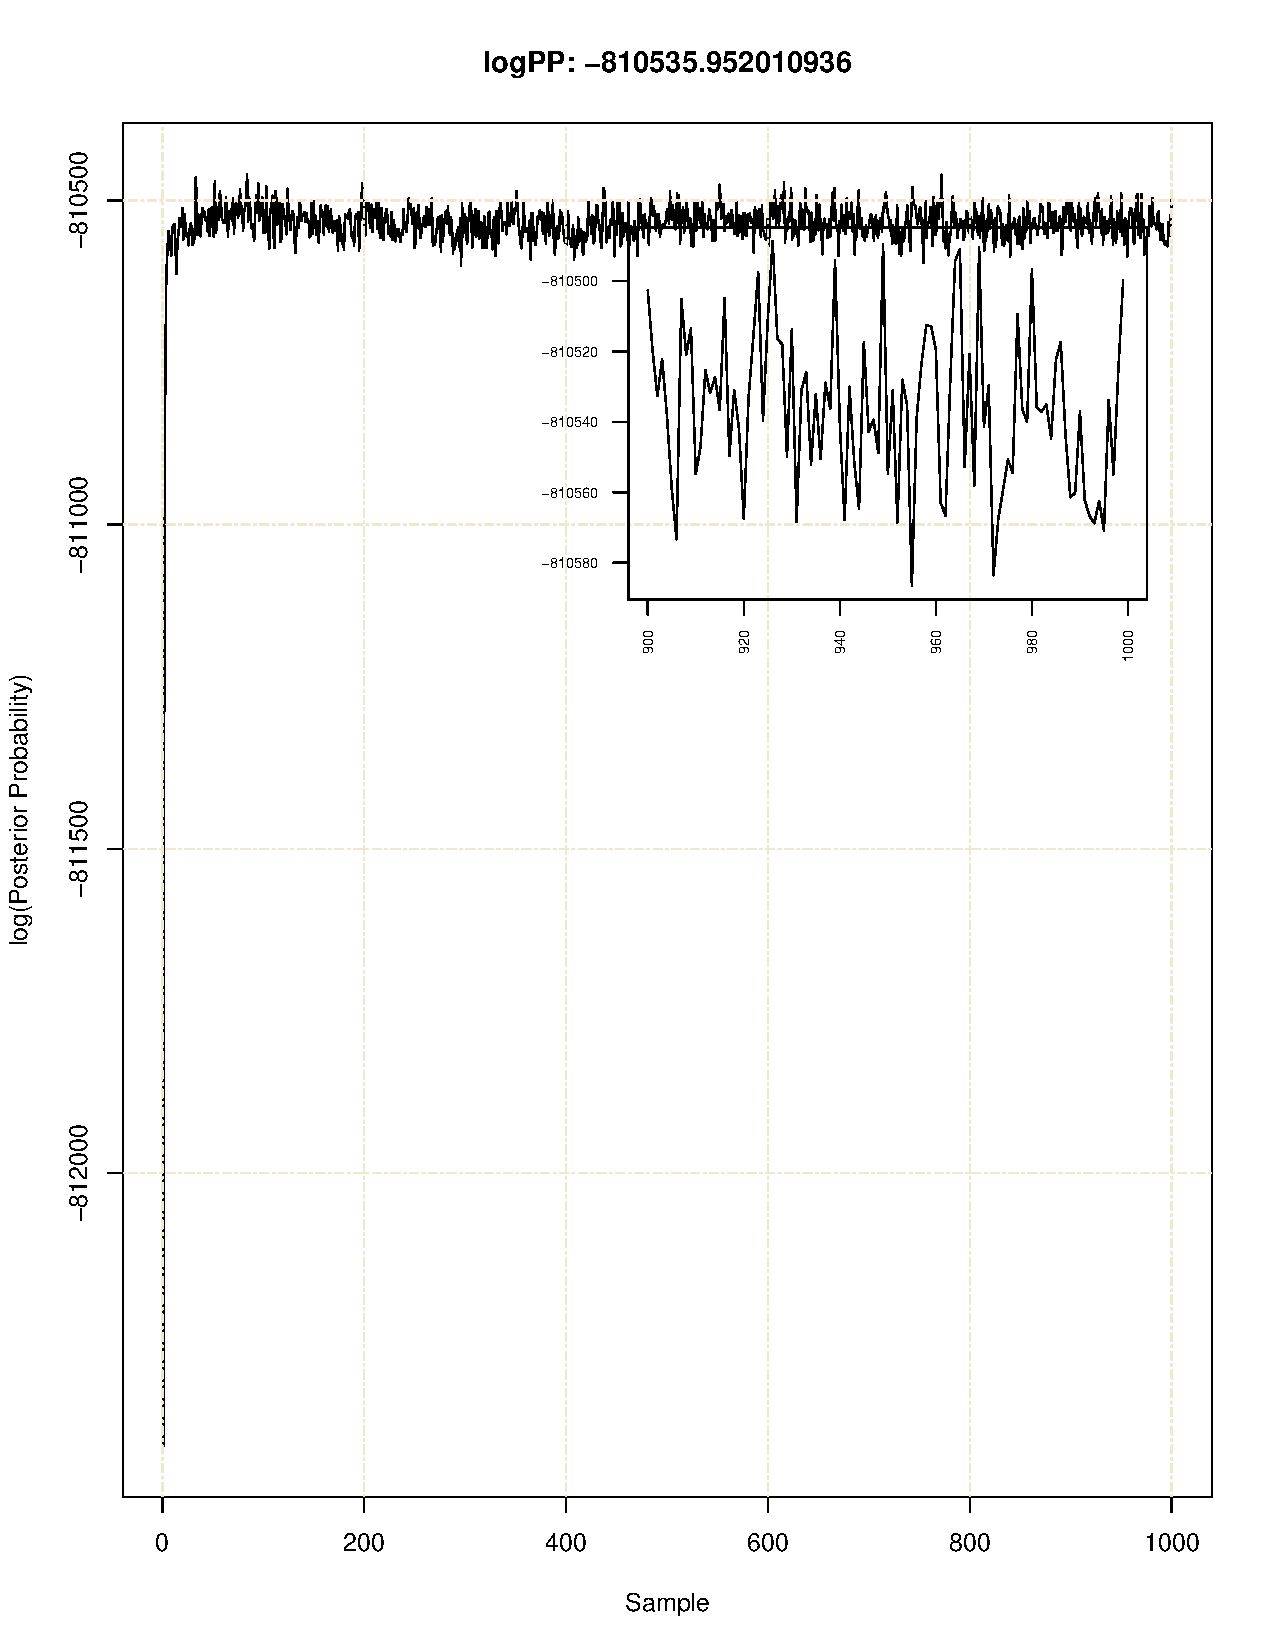
\includegraphics[scale=.65]{FONSE_Plots/2016/June_27/ROC/Run1_LogLikeTrace}
        \caption{LogLikelihood trace for ROC}
        \label{fig:JUN27_RLOG}
    \end{figure}
    \begin{figure}
        \centering
        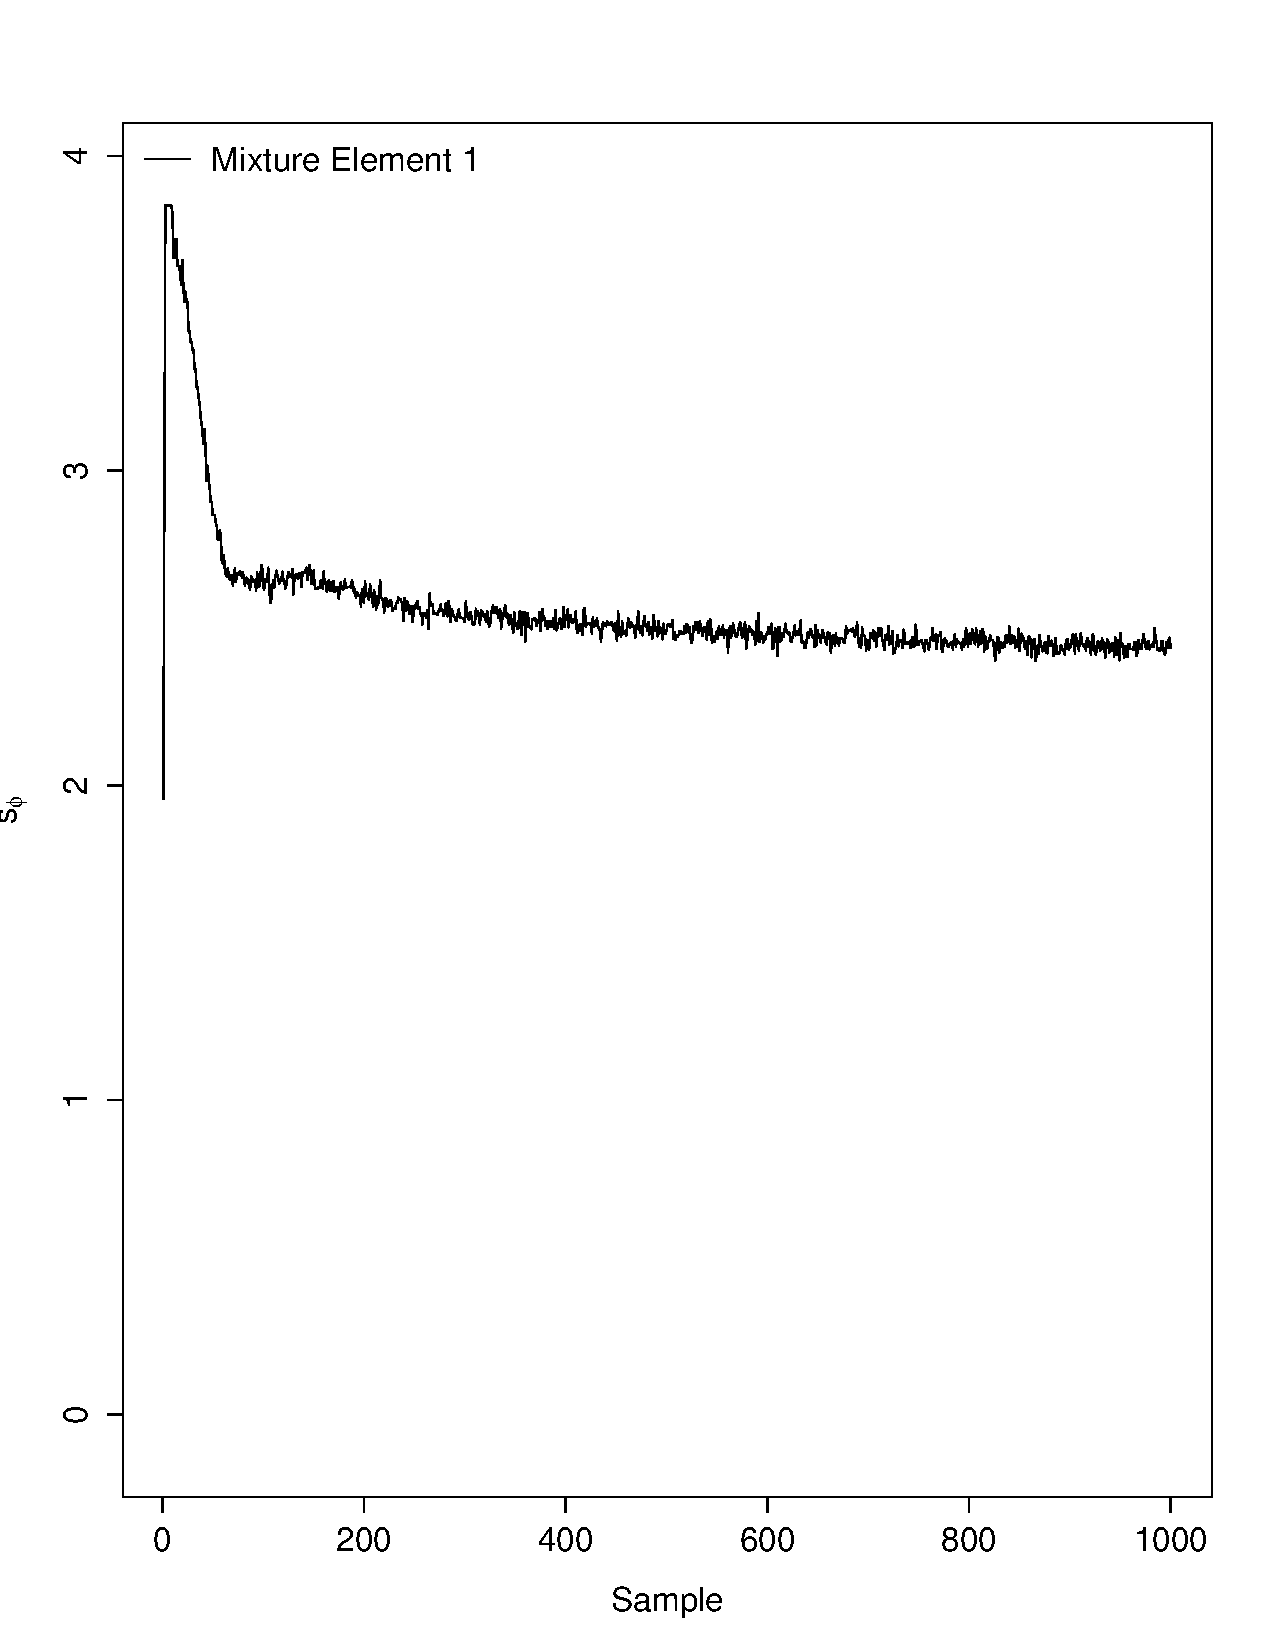
\includegraphics[scale=.65]{FONSE_Plots/2016/June_27/Run1_SphiTrace}
        \caption{Sphi trace for FONSE}
        \label{fig:JUN27_FSPHI}
    \end{figure}
    \begin{figure}
        \centering
        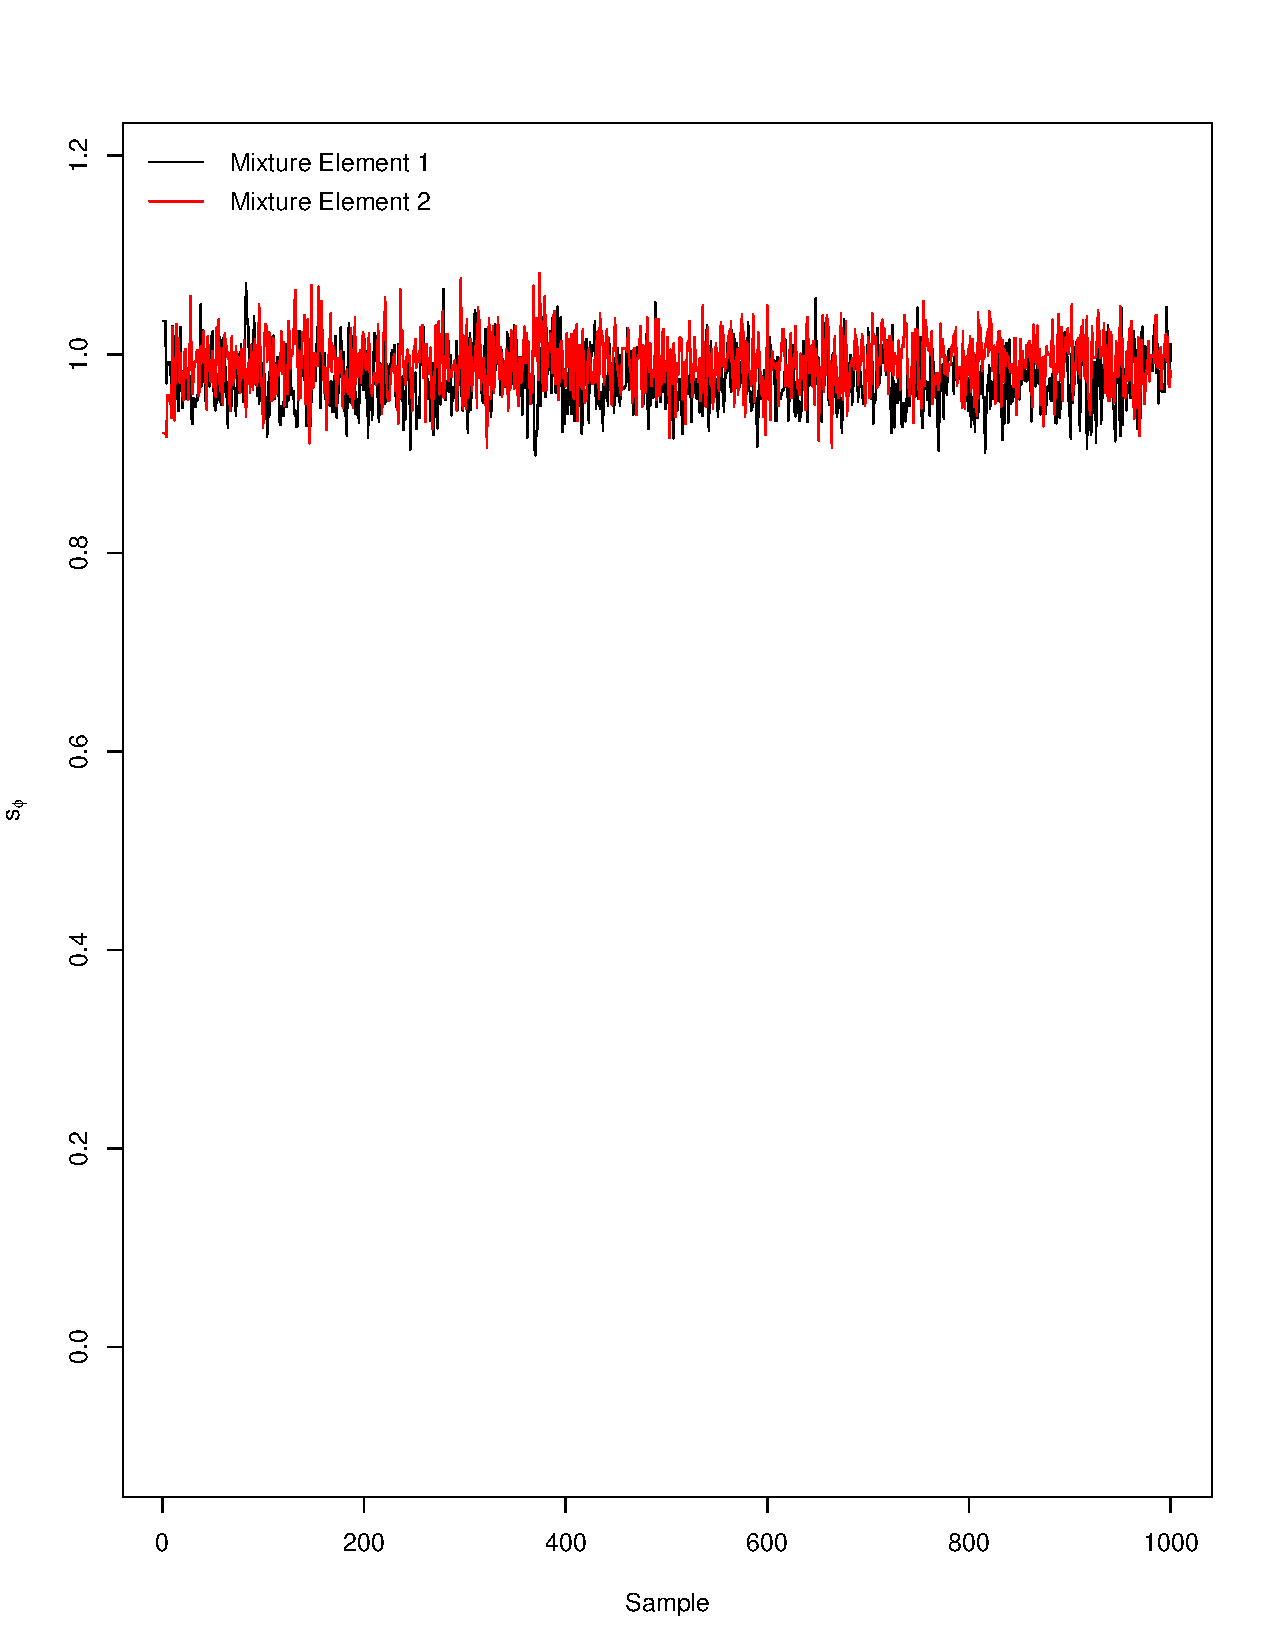
\includegraphics[scale=.65]{FONSE_Plots/2016/June_27/ROC/Run1_SphiTrace}
        \caption{Sphi trace for ROC}
        \label{fig:JUN27_RSPHI}
    \end{figure}
    \begin{figure}
        \centering
        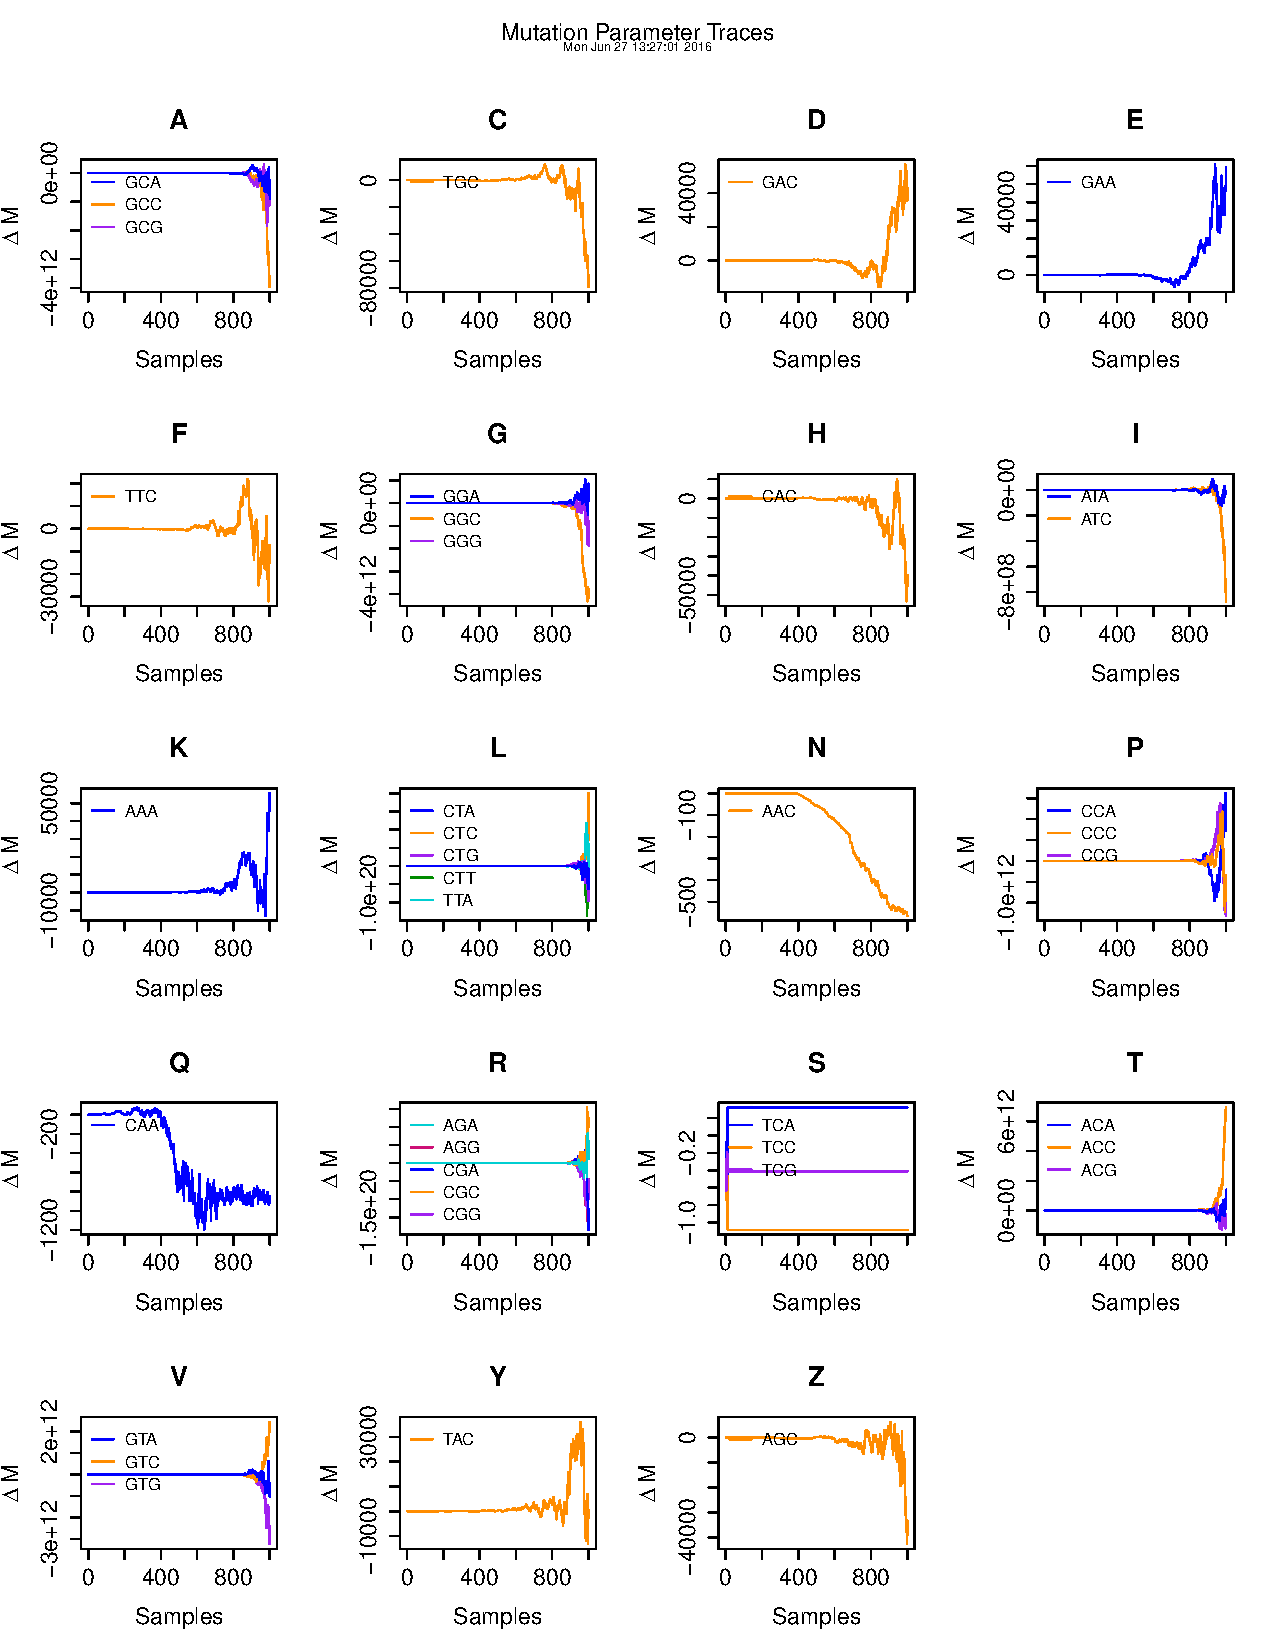
\includegraphics[scale=.65]{FONSE_Plots/2016/June_27/Run1_MutationTrace}
        \caption{Mutation trace for FONSE}
        \label{fig:JUN27_FMUT}
    \end{figure}
    \begin{figure}
        \centering
        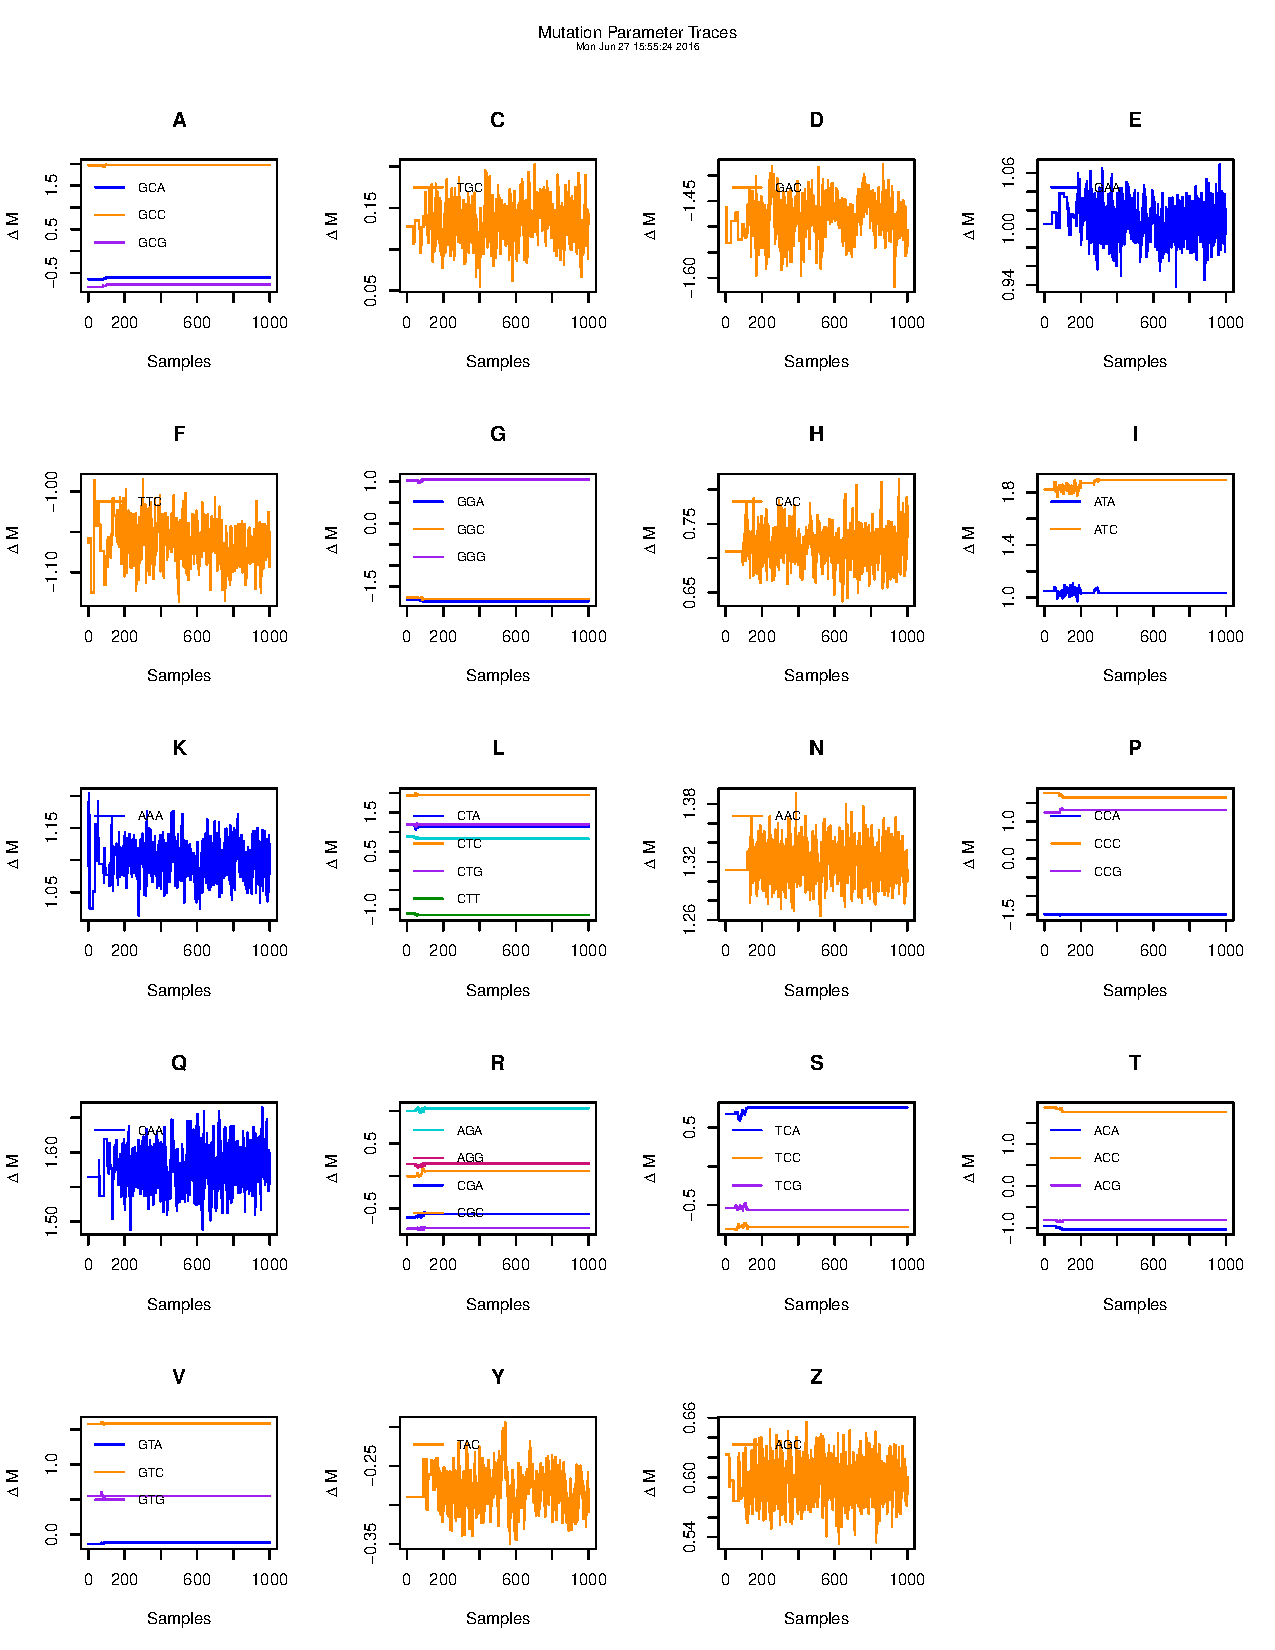
\includegraphics[scale=.65]{FONSE_Plots/2016/June_27/ROC/Run1_MutationTrace}
        \caption{Mutation trace for ROC}
        \label{fig:JUN27_RMUT}
    \end{figure}
    \begin{figure}
        \centering
        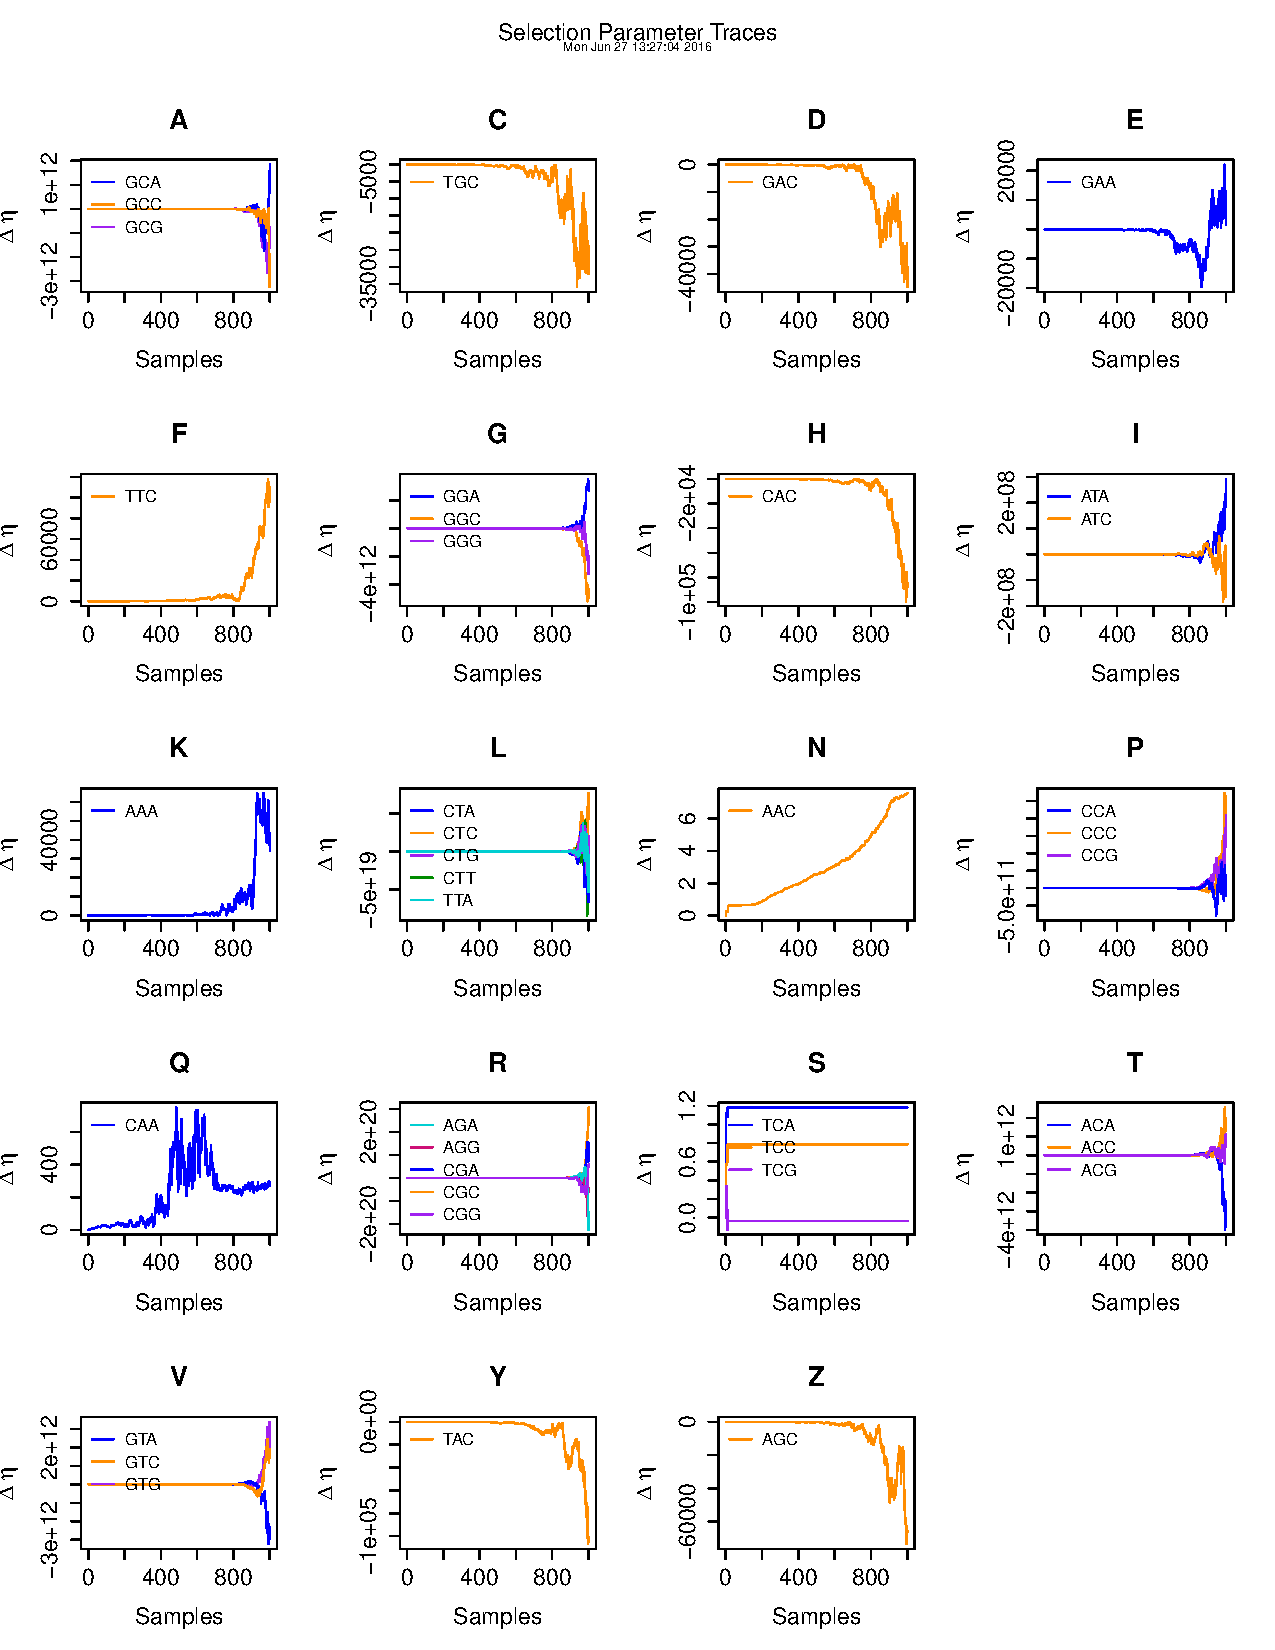
\includegraphics[scale=.65]{FONSE_Plots/2016/June_27/Run1_SelectionTrace}
        \caption{Selection trace for FONSE}
        \label{fig:JUN27_FSEL}
    \end{figure}
    \begin{figure}
        \centering
        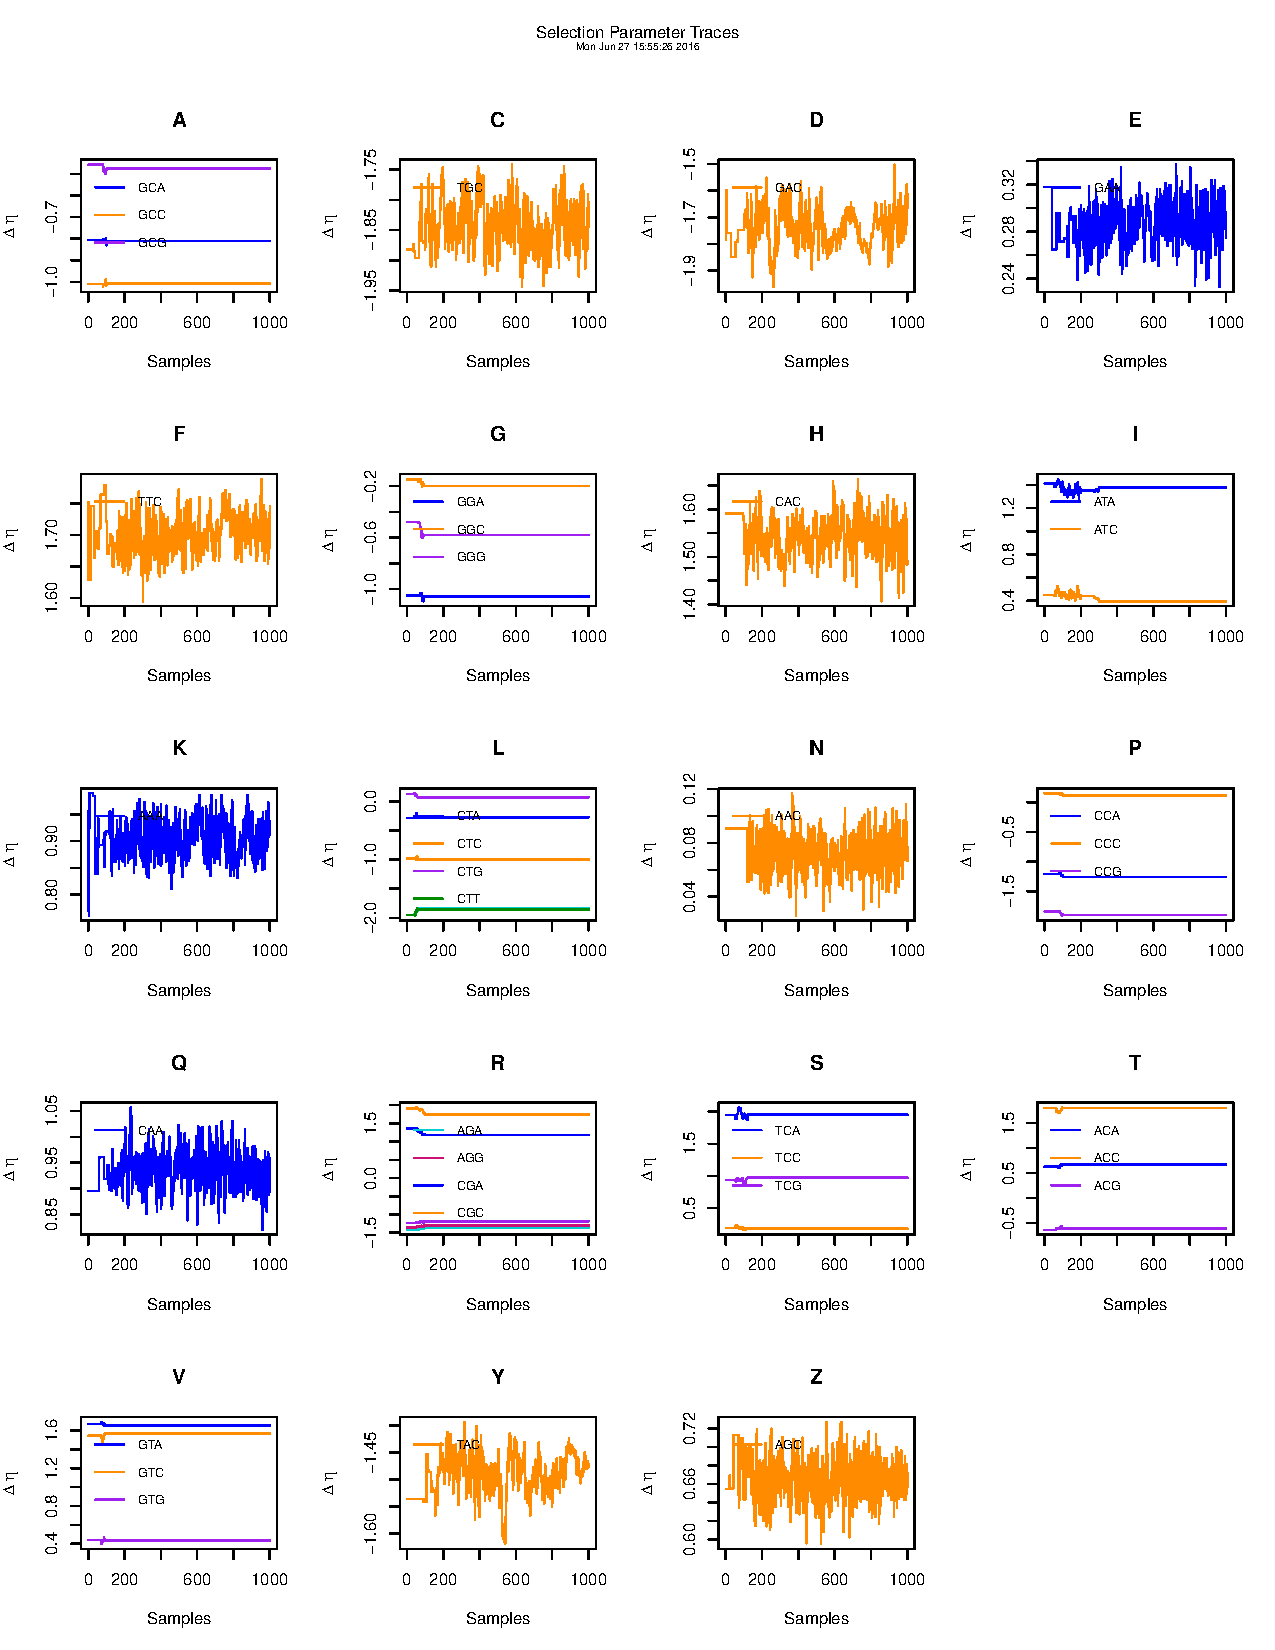
\includegraphics[scale=.65]{FONSE_Plots/2016/June_27/ROC/Run1_SelectionTrace}
        \caption{Selection trace for ROC}
        \label{fig:JUN27_RSEL}
    \end{figure}
    
\labday{June 29, 2016}
    \begin{itemize}
        \item The main focus of today was on implementing the option to control what portion of the log likelihood trace is zoomed in. With this it will now be possible to observe the behavior of the log likelihood at the earlier stages instead of being able to observe just the drop.
\footnote{mikeg: 6/30/16 -- was all of this effort necessary?
  Could you not have just simply plotted the traces on their own? 
  Doing them as an inset means the 10 plots of interest are spread over 10 pages rather than simply plotting them all as a grid on one page.}
\footnote{aland: Attempting to plot just certain portions of the trace led to plots that didn't show any information at all. I tried to research how to properly alter the plot function call to get what I wanted, but after being unsuccessful, I decided it would be easier to just alter the zoom and adding that option would be a benefit for further testing.}
  
        \item Ran FONSE with b = 0.001, samples = 1000, and thinning = 10 in order to get the zoomed in traces for each tenth of the trace. Looking at these it appears that the dropping starts fairly early and continues to drop at slightly increasing rates until the MCMC loop ends as shown in figures.
\footnote{mikeg: 6/30/16 -- I would argue that these drops in the LLik are really fast! 
  Each window has a huge increas in the order of magnitude of the drops.
  The first is E-5 and by the end it's dropping to E40 all within a 100 steps.
}
\footnote{mikeg: 6/30/16 -- So this tells us that the algorithm is misbehaving from the get go.  
  Why are the acceptance ratios either 1 or 0?
  Why are they 1 when the LLik is worse than the current state?
  We need to fix this bug.
}
\footnote{aland: After confering with Cedric, he feels that the most likely reason would be a problem with the covariance matrix, (something I need to familiarize myself with more. We mentioned only updating and using the diagonal, but I feel getting the individual AA traces in would be more effective in discovering the issue.}
    \end{itemize}
    \begin{figure}
        \centering
        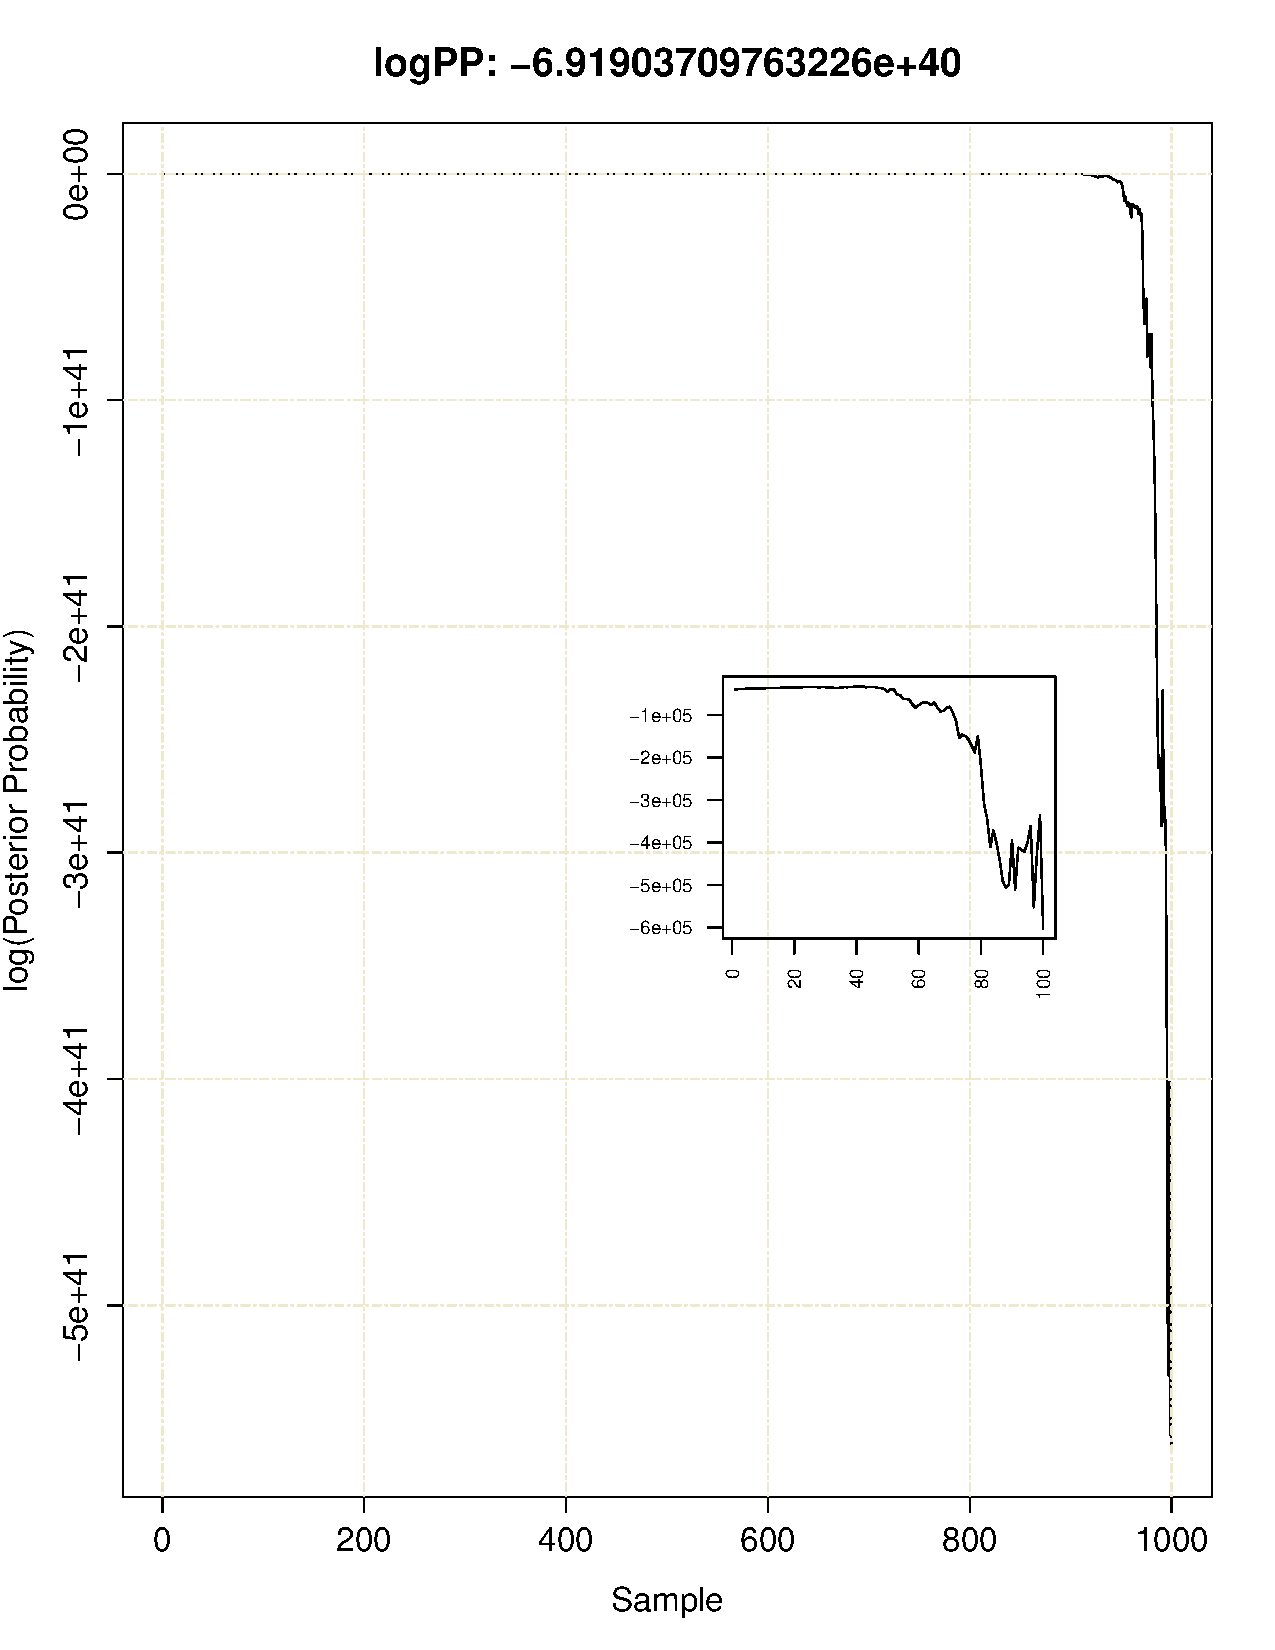
\includegraphics[scale=.75]{FONSE_Plots/2016/June_29/LogLikeTrace_1-100}
        \caption{Log Likelihood trace with the zoom at 1-100}
        \label{fig:JUN29_1-100}
    \end{figure}
    \begin{figure}
        \centering
        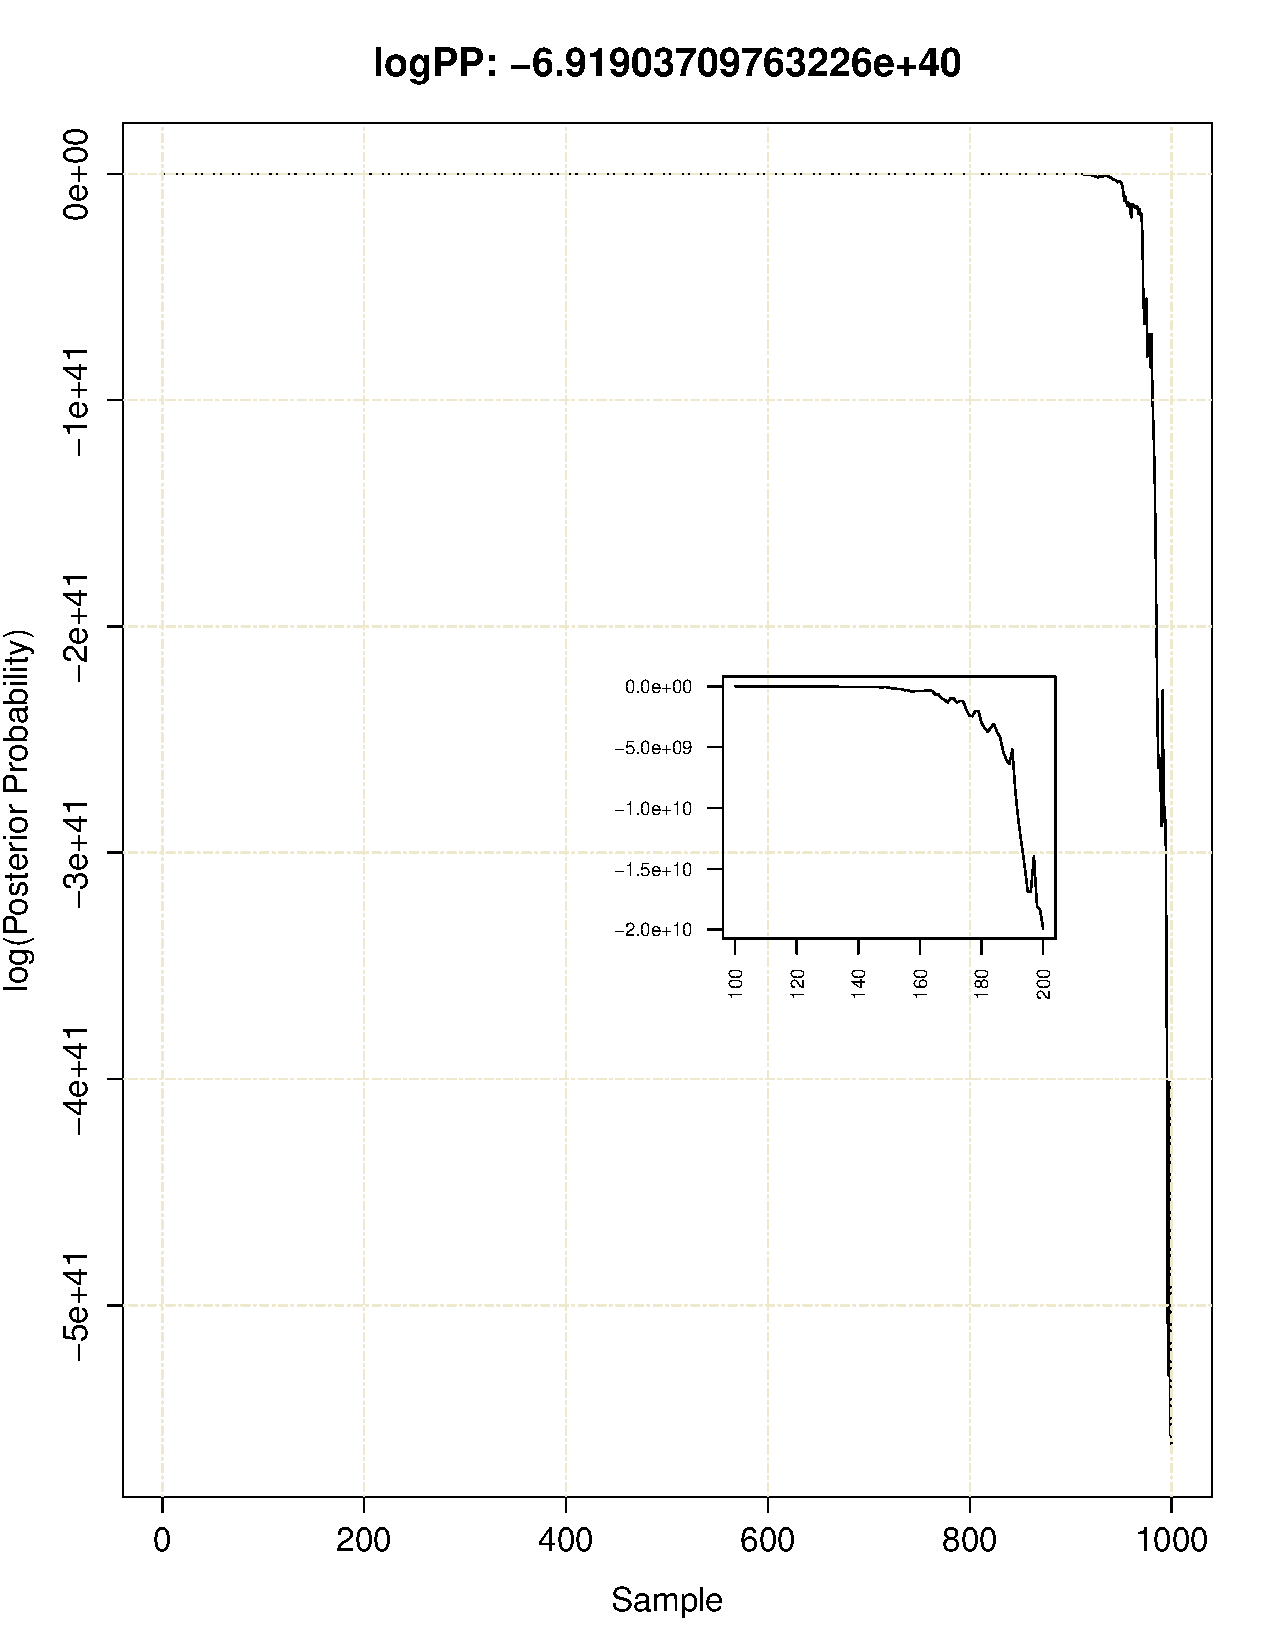
\includegraphics[scale=.75]{FONSE_Plots/2016/June_29/LogLikeTrace_100-200}
        \caption{Log Likelihood trace with the zoom at 100-200}
        \label{fig:JUN29_100-200}
    \end{figure}
    \begin{figure}
        \centering
        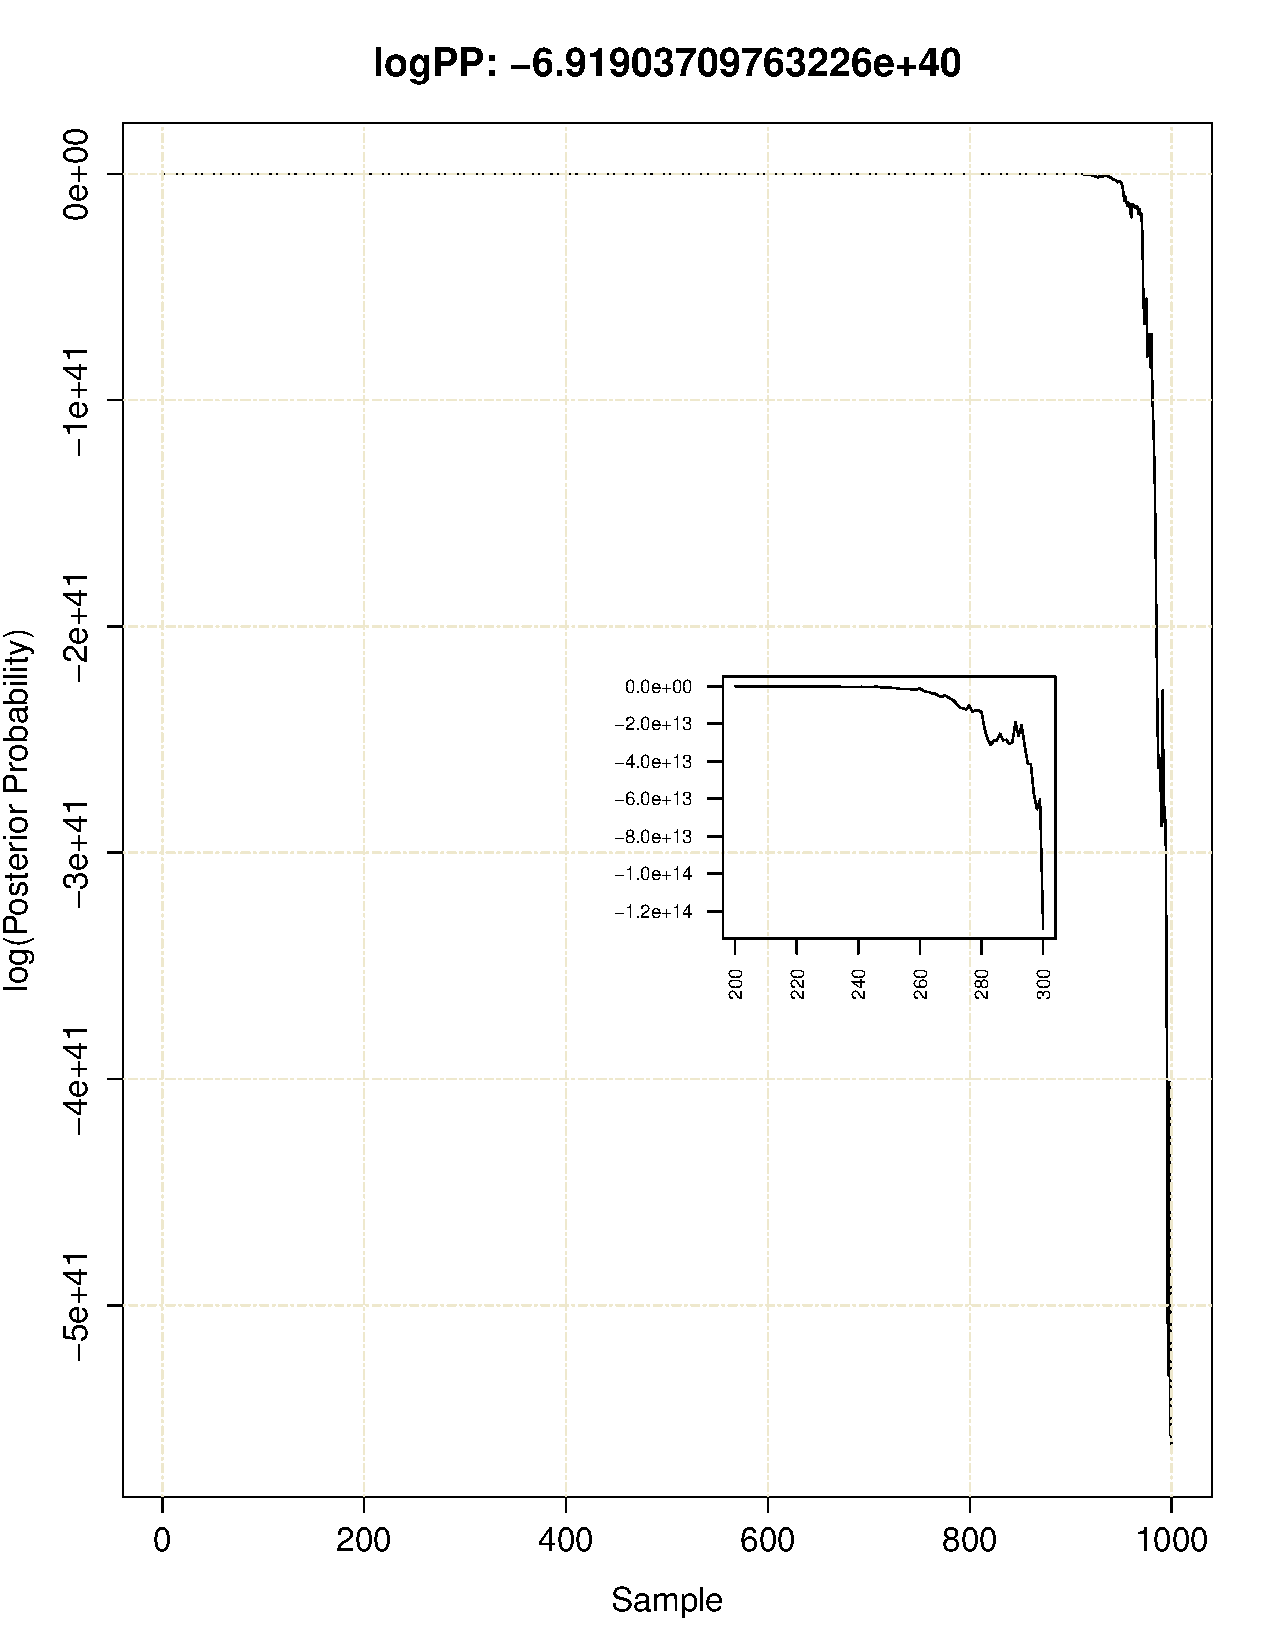
\includegraphics[scale=.75]{FONSE_Plots/2016/June_29/LogLikeTrace_200-300}
        \caption{Log Likelihood trace with the zoom at 200-300}
        \label{fig:JUN29_200-300}
    \end{figure}
    \begin{figure}
        \centering
        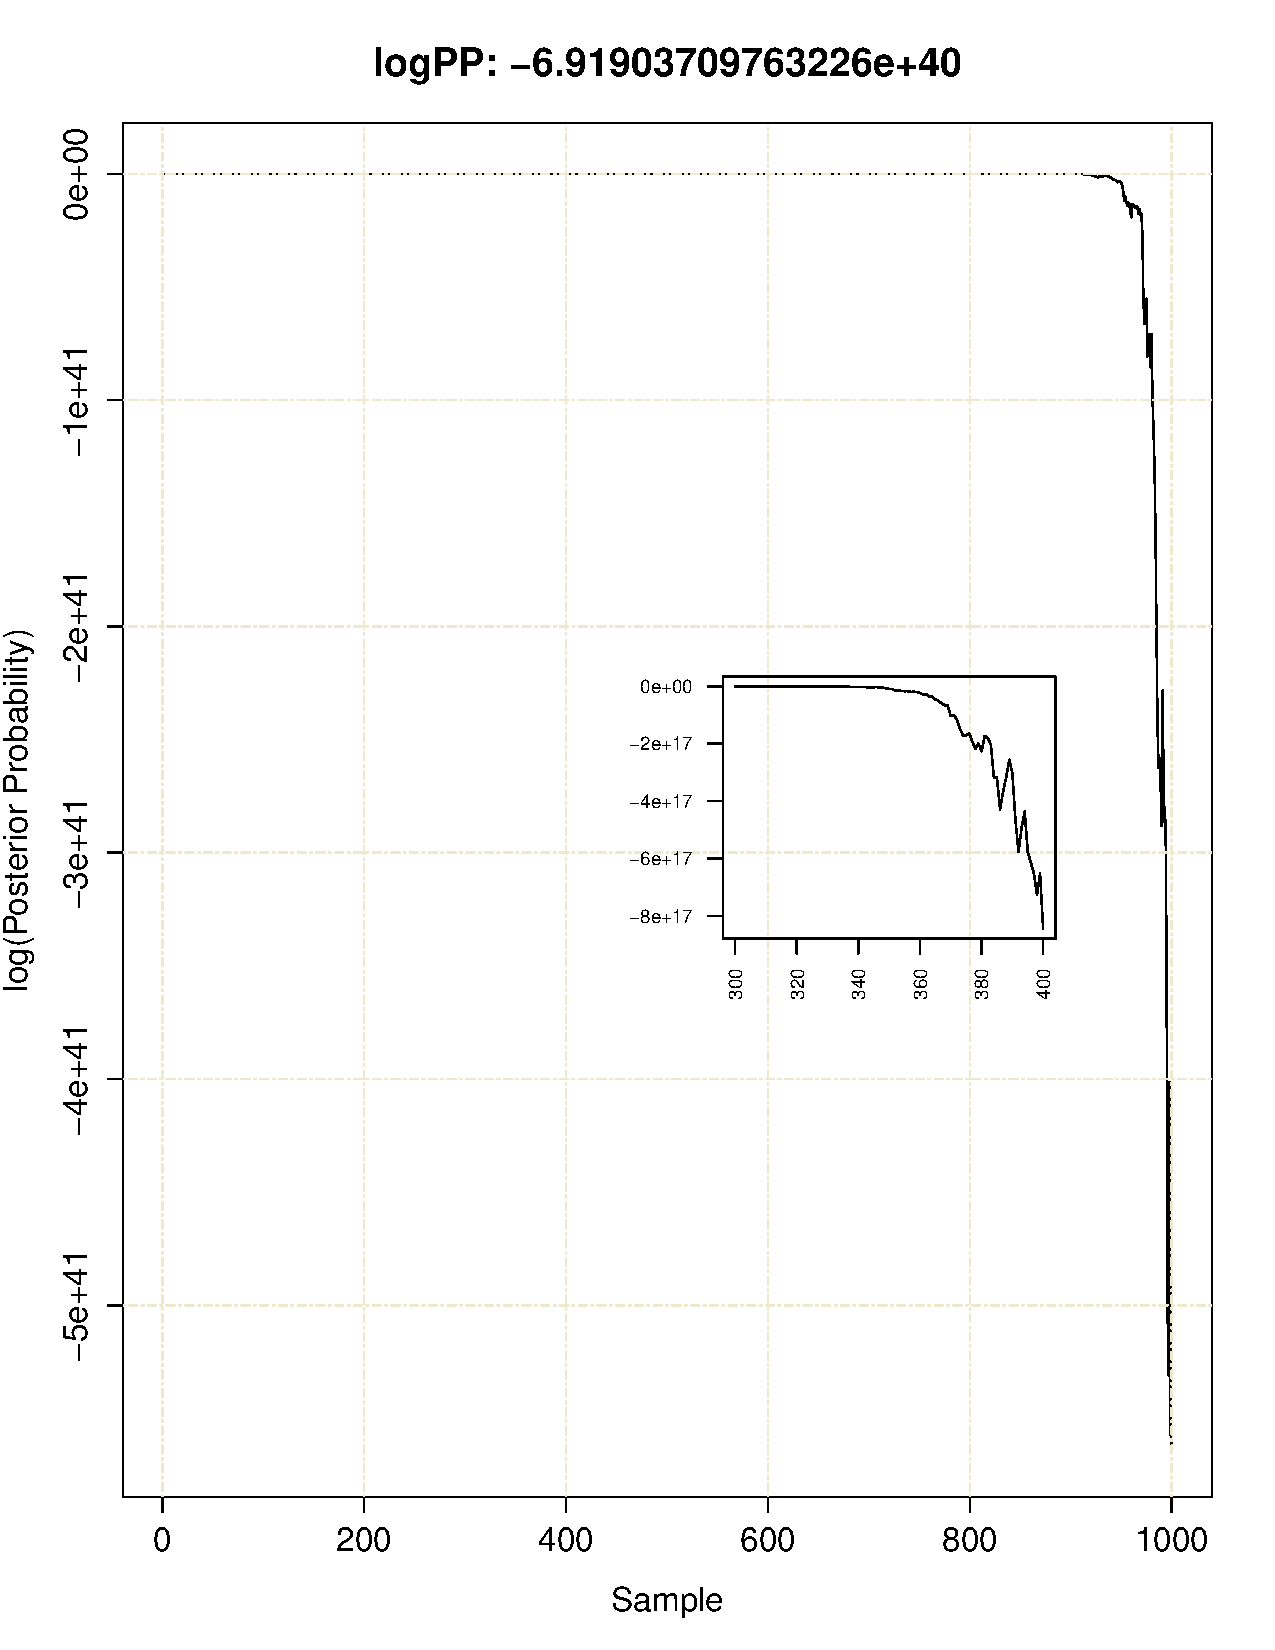
\includegraphics[scale=.75]{FONSE_Plots/2016/June_29/LogLikeTrace_300-400}
        \caption{Log Likelihood trace with the zoom at 300-400}
        \label{fig:JUN29_300-400}
    \end{figure}
    \begin{figure}
        \centering
        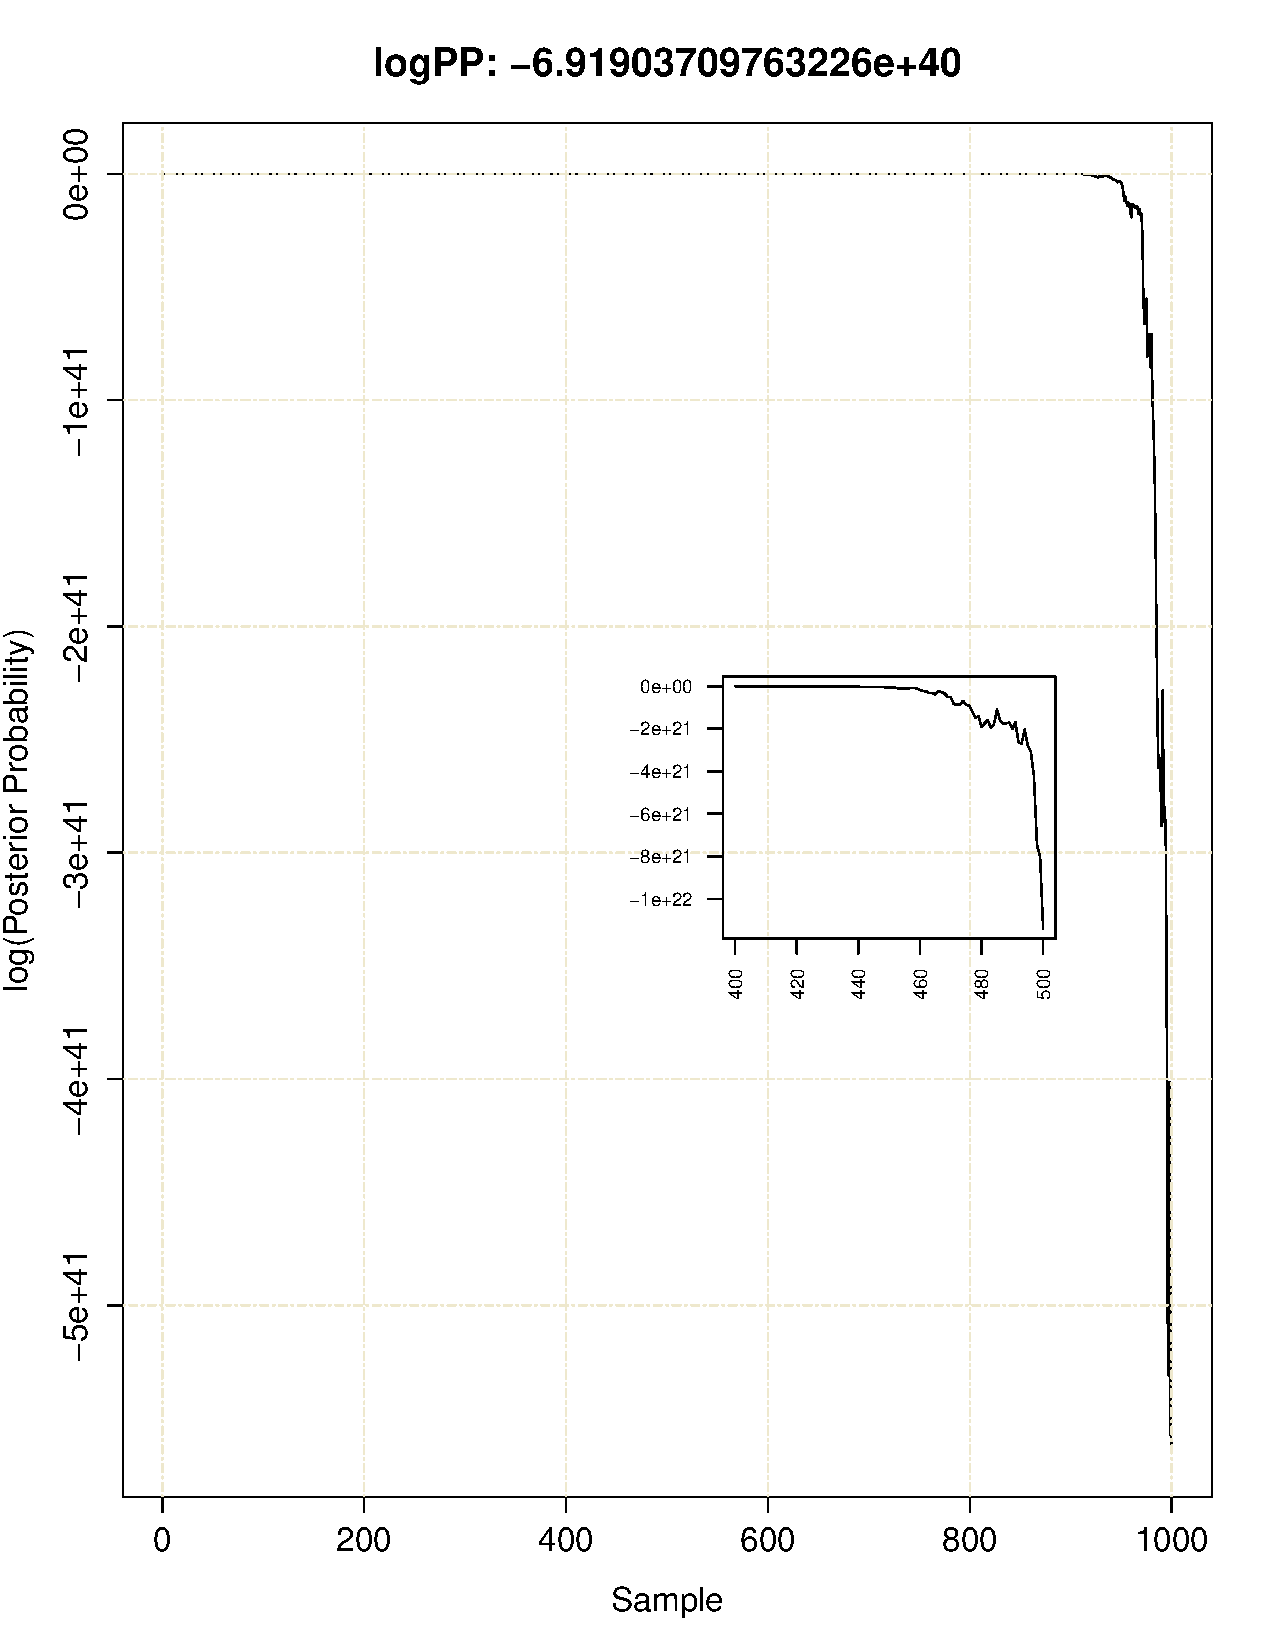
\includegraphics[scale=.75]{FONSE_Plots/2016/June_29/LogLikeTrace_400-500}
        \caption{Log Likelihood trace with the zoom at 400-500}
        \label{fig:JUN29_400-500}
    \end{figure}
    \begin{figure}
        \centering
        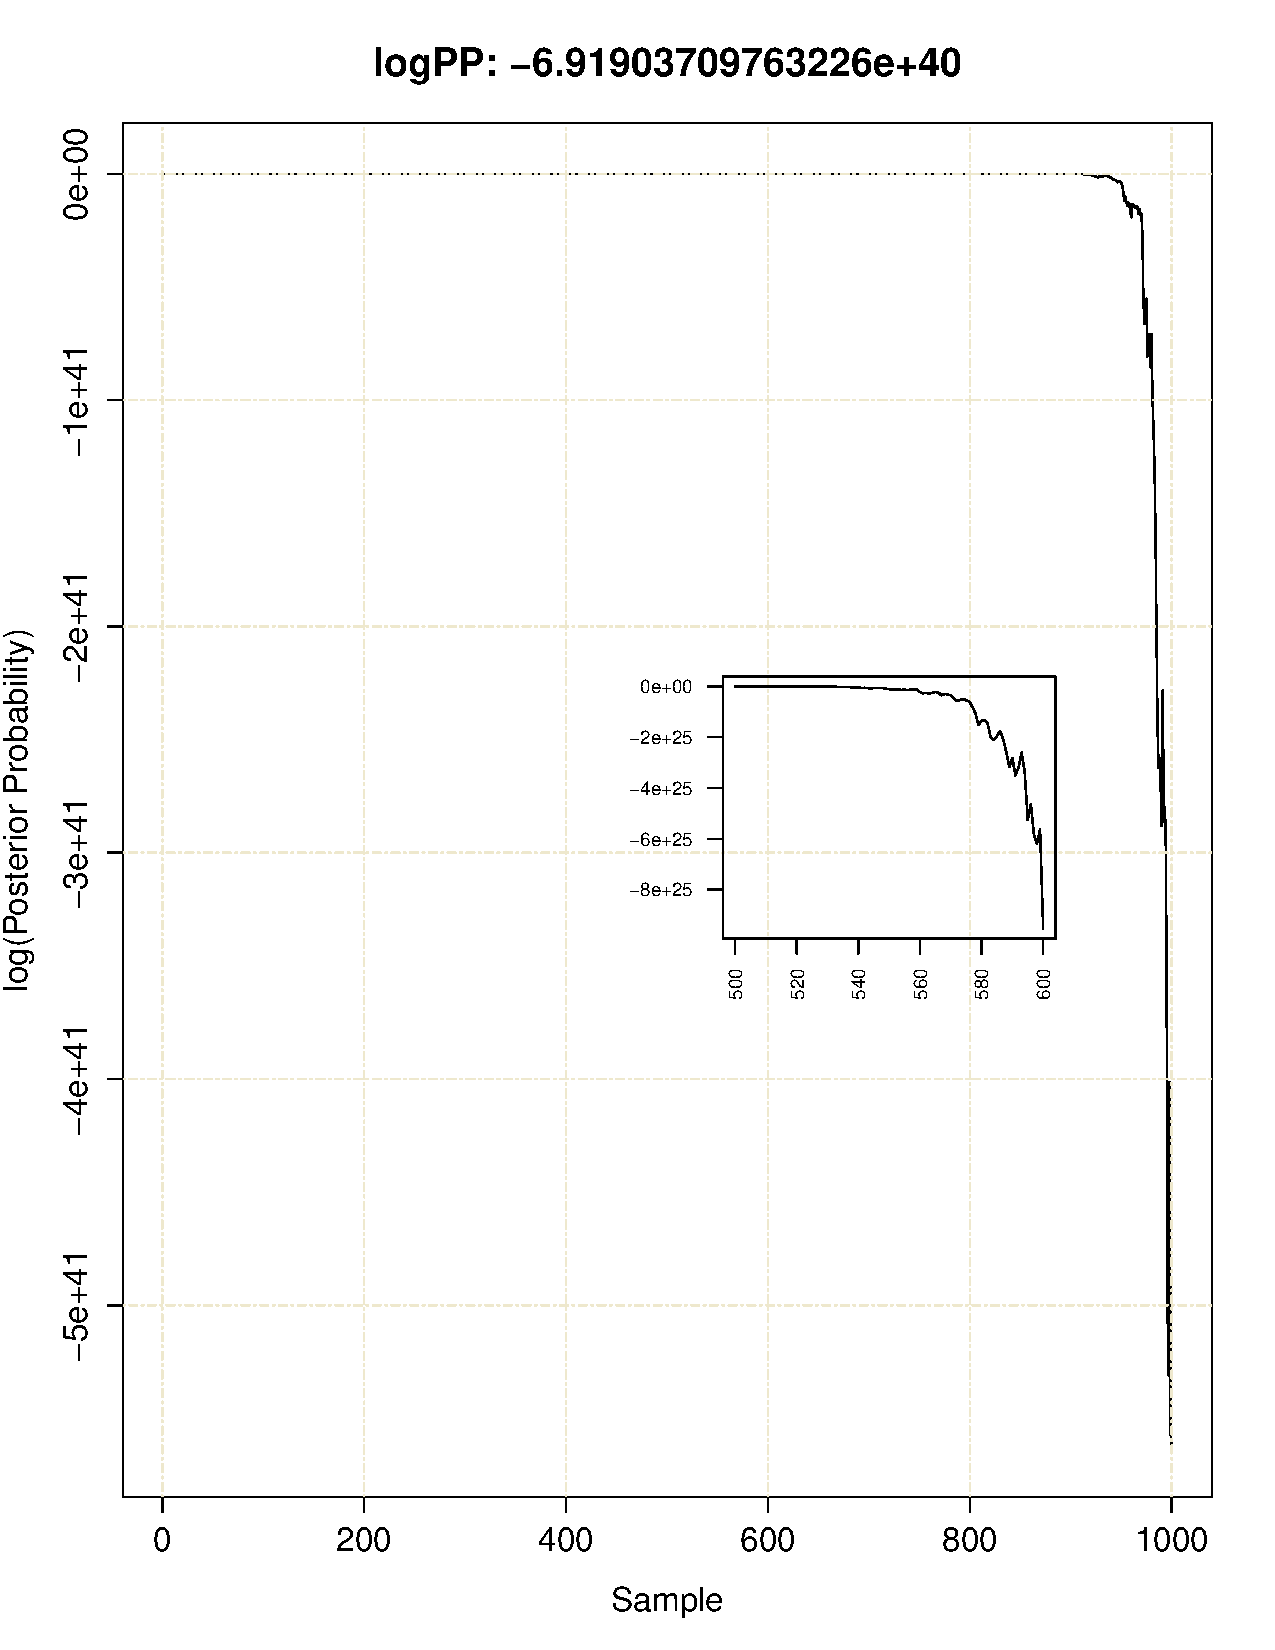
\includegraphics[scale=.75]{FONSE_Plots/2016/June_29/LogLikeTrace_500-600}
        \caption{Log Likelihood trace with the zoom at 500-600}
        \label{fig:JUN29_500-600}
    \end{figure}
    \begin{figure}
        \centering
        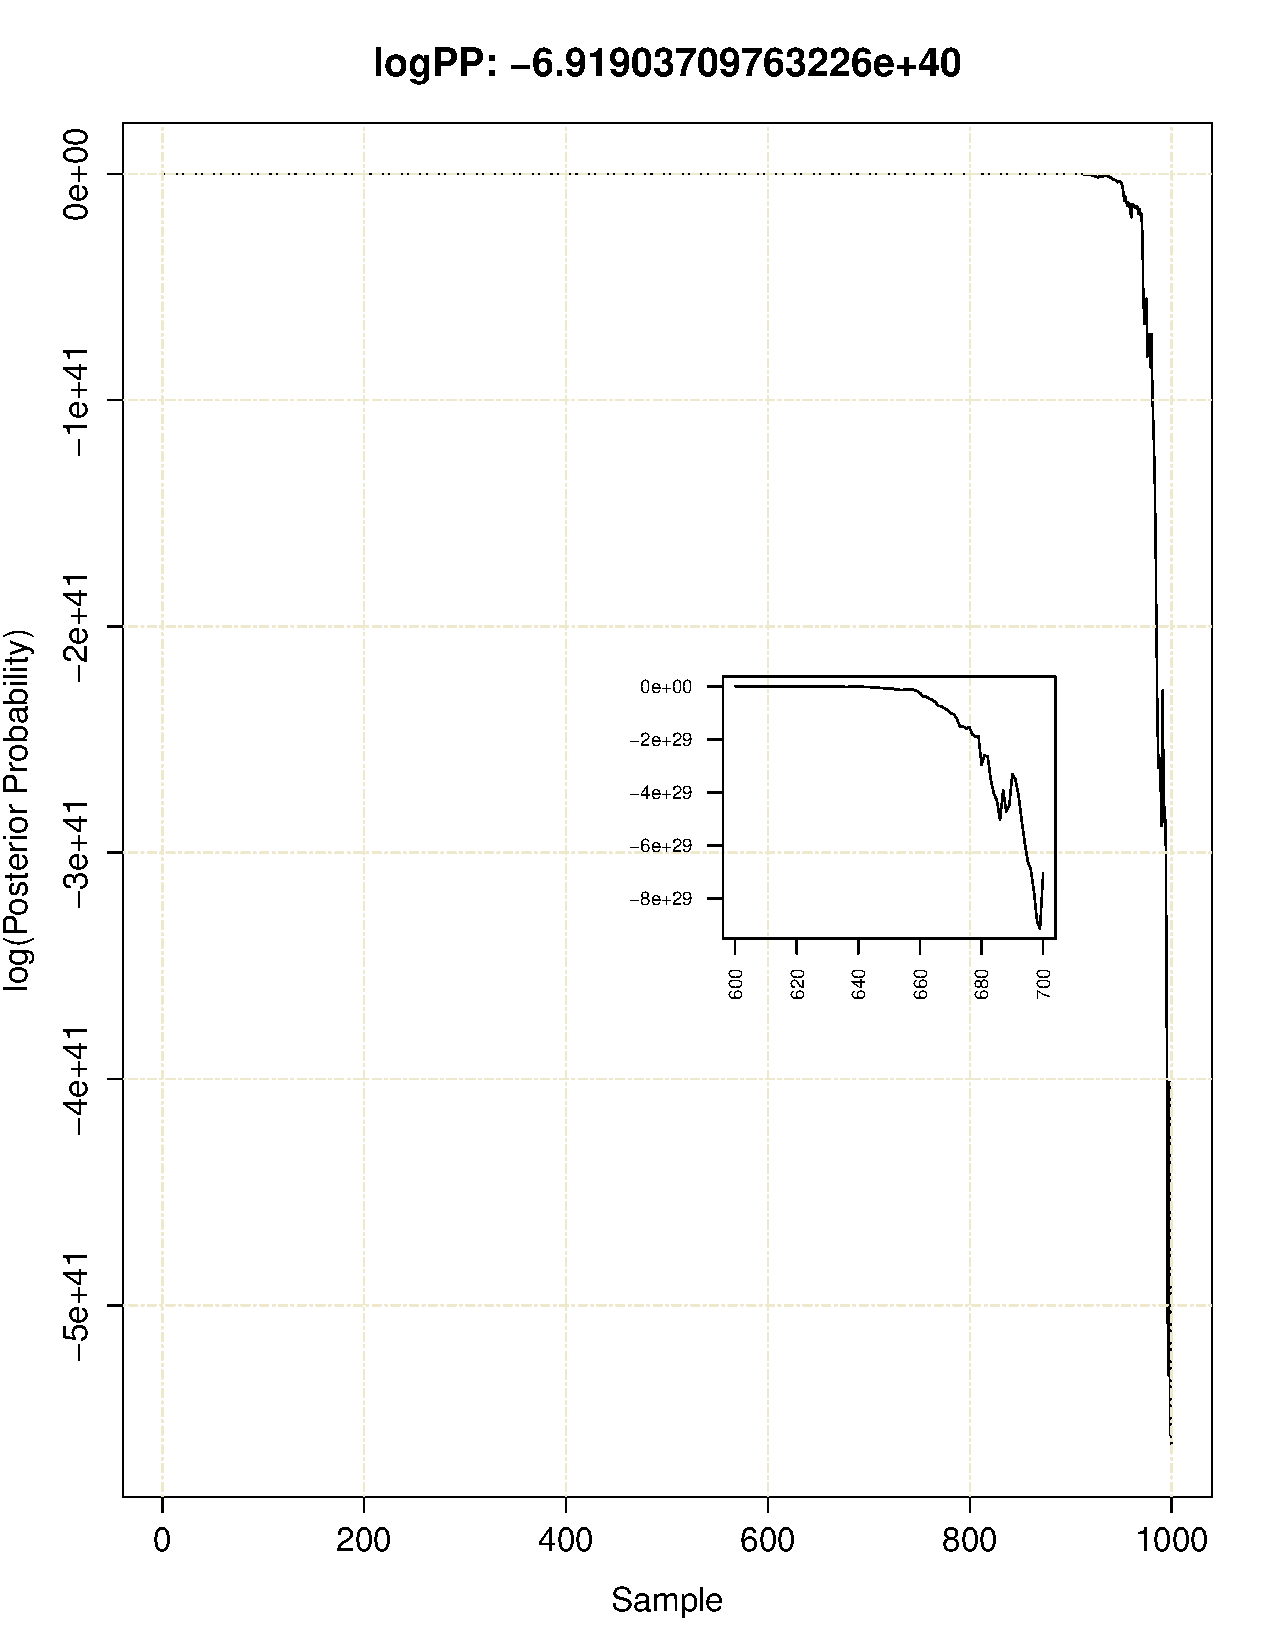
\includegraphics[scale=.75]{FONSE_Plots/2016/June_29/LogLikeTrace_600-700}
        \caption{Log Likelihood trace with the zoom at 600-700}
        \label{fig:JUN29_600-700}
    \end{figure}
    \begin{figure}
        \centering
        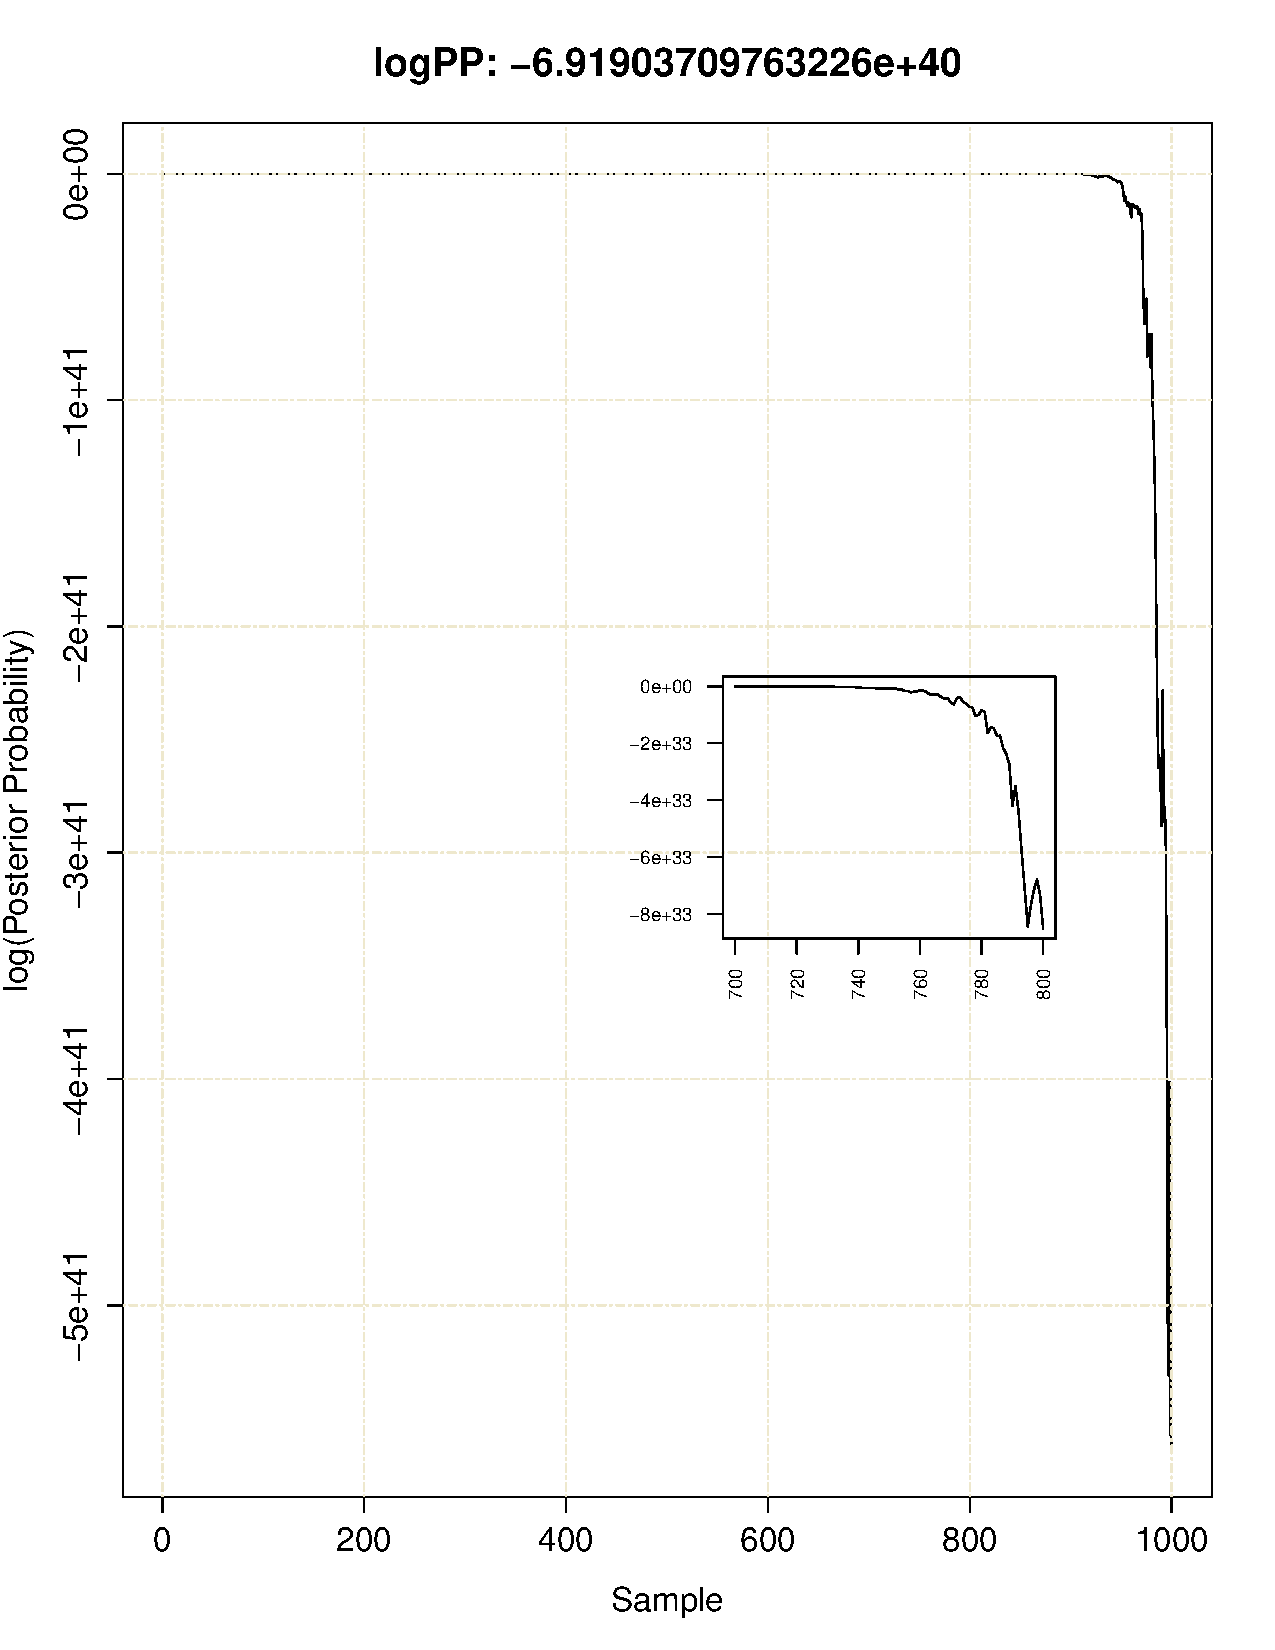
\includegraphics[scale=.75]{FONSE_Plots/2016/June_29/LogLikeTrace_700-800}
        \caption{Log Likelihood trace with the zoom at 700-800}
        \label{fig:JUN29_700-800}
    \end{figure}
    \begin{figure}
        \centering
        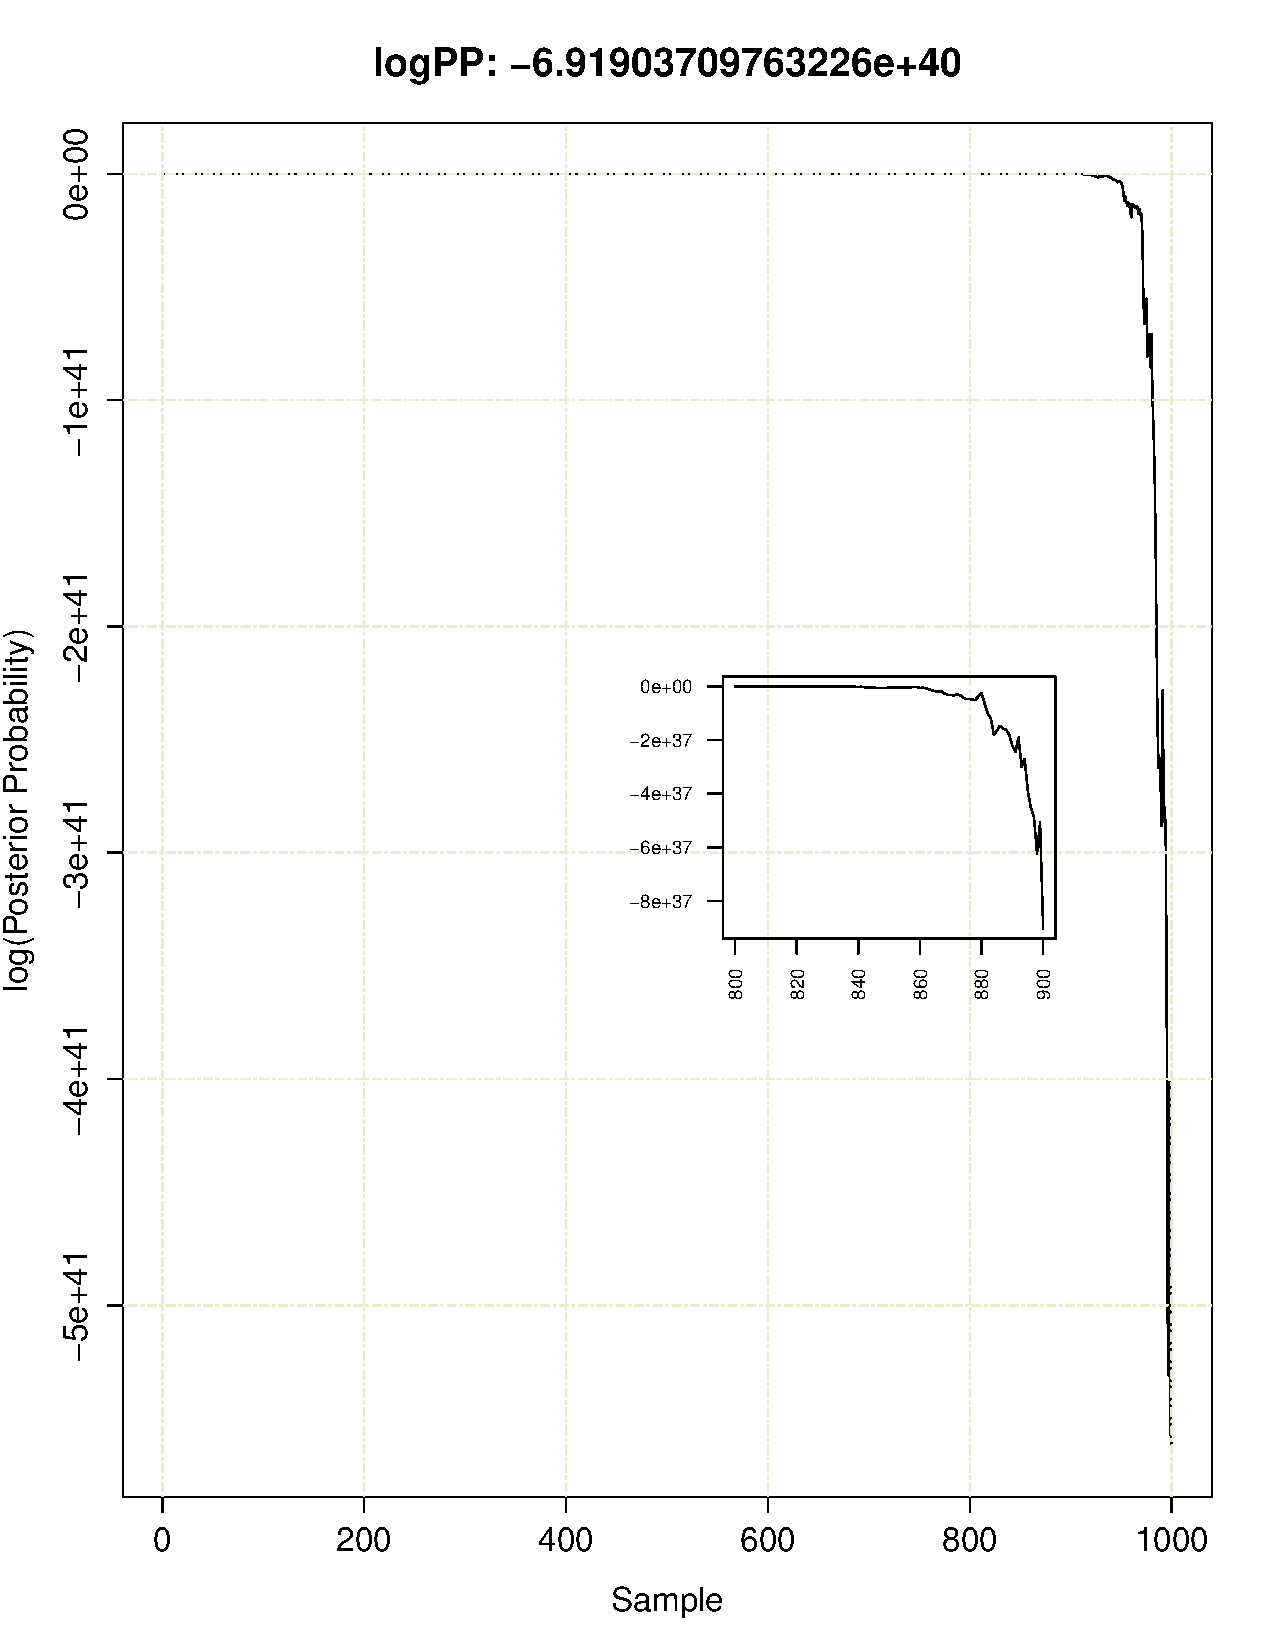
\includegraphics[scale=.75]{FONSE_Plots/2016/June_29/LogLikeTrace_800-900}
        \caption{Log Likelihood trace with the zoom at 800-900}
        \label{fig:JUN29_800-900}
    \end{figure}
    \begin{figure}
        \centering
        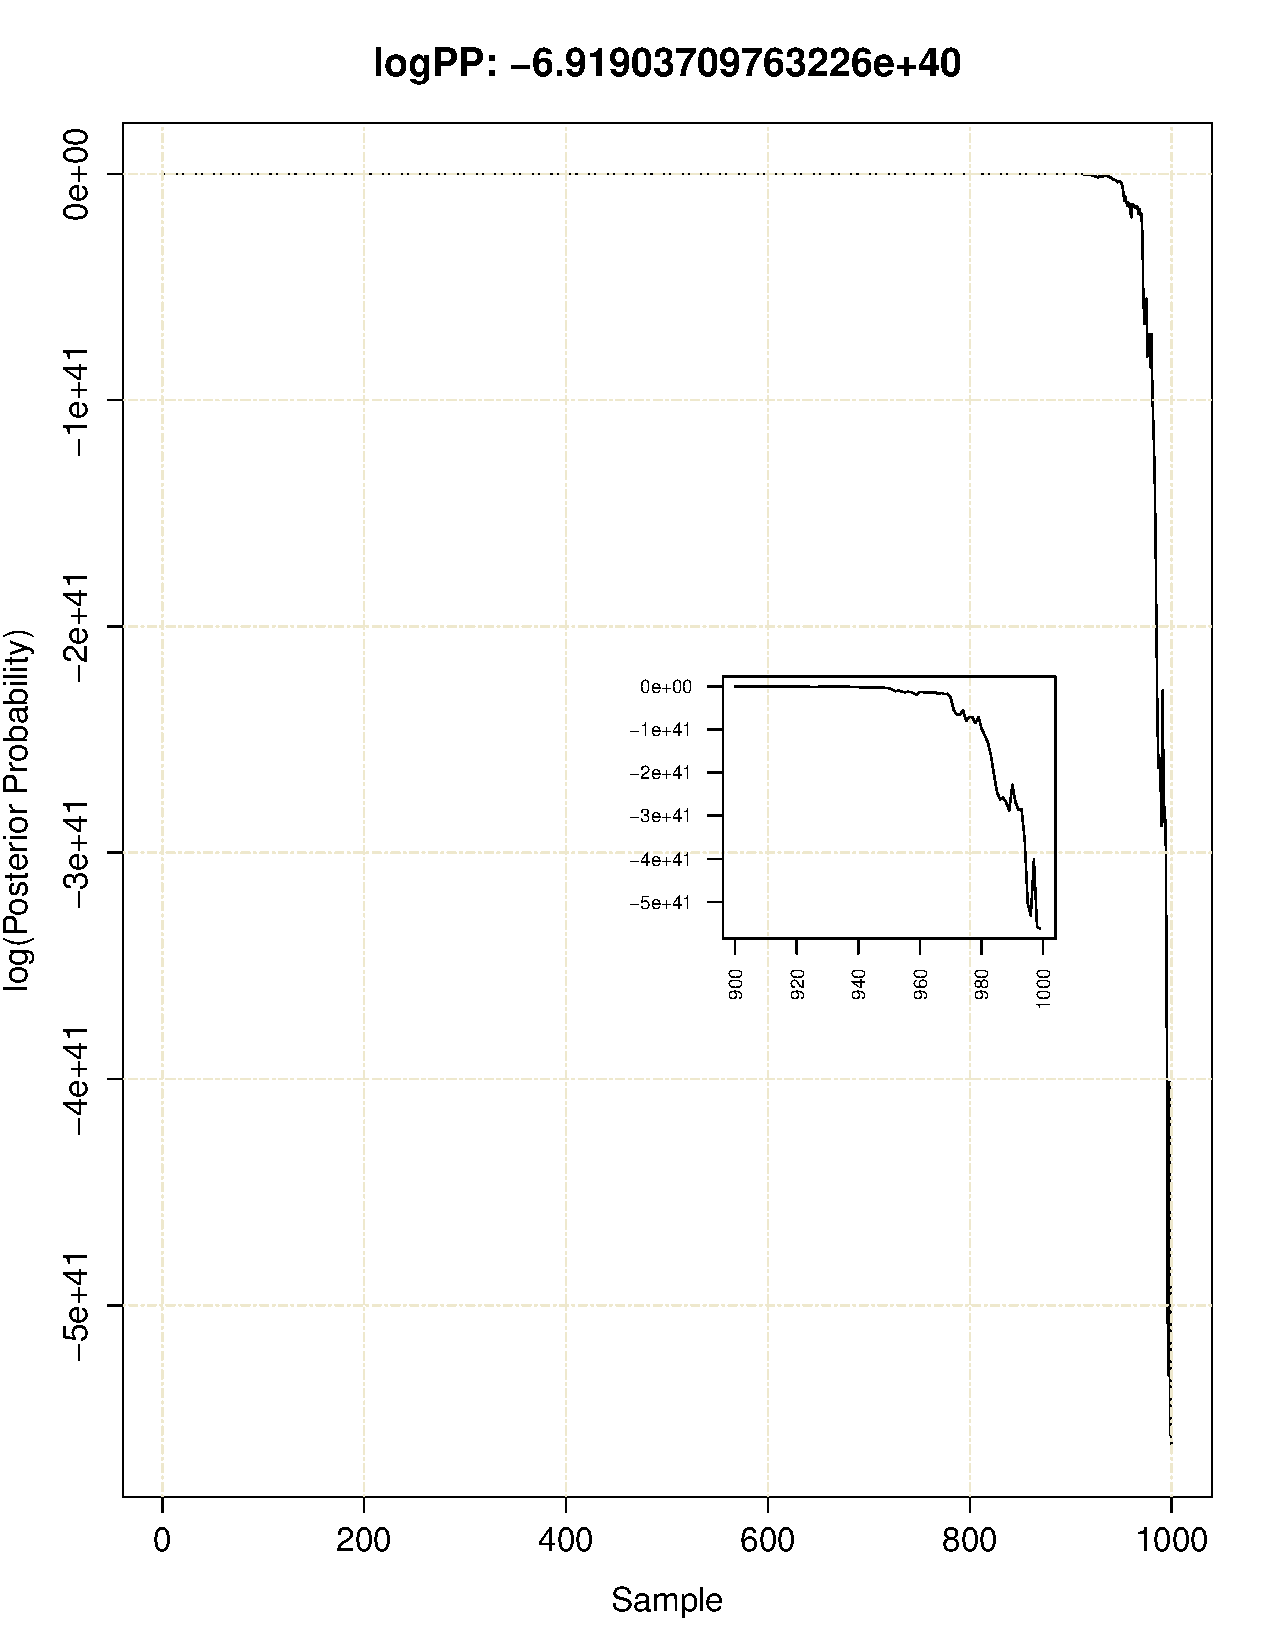
\includegraphics[scale=.75]{FONSE_Plots/2016/June_29/LogLikeTrace_900-1000}
        \caption{Log Likelihood trace with the zoom at 900-1000}
        \label{fig:JUN29_900-1000}
    \end{figure}
    
\labday{June 30, 2016}
    \begin{itemize}
        \item While combing the code for the MCMC algorithm I noticed that for the large part, arrays were being used instead of vectors, and while iterating through both takes about the same amount of time and vectors have a slightly larger base overhead due to them keeping track of their own sizes, the arrays were being initialized inside of a loop by using calls to "new". Since this loop iterates "numGenes" times, every iteration caused six arrays to be declared with "new" and then deleted with "delete" at the end of the loop, leading to enormous overhead, so I ran FONSE on my laptop to get a control time and changed all of the arrays in the acceptRejectSynthesisRateLevelForAllGenes function in MCMCAlgorithm.cpp to vectors and reran FONSE twice.
        \item Run 1: b = 0.001, samples = 1000, thinning = 10 with arrays.
            \begin{itemize}
                \item The MCMC loop for FONSE ran for 5708.03 seconds
                \item I defined the rate as iterations/second and since the loop ran for 10000 iterations, the rate for the first was ~1.75 iterations/second.
            \end{itemize}
        \item Runs 2 \& 3: same as run 1 but with vectors instead of arrays
            \begin{itemize}
                \item The loop ran first for 3832.63 seconds then for 3859.51 seconds for an average of 3846.07
                \item The rate consequently was 2.6 iterations per second
            \end{itemize}
        \item Although one run with arrays and two with vectors isn't quite enough to confirm how much faster the algorithm for FONSE now is, initial results suggest that the algorithm is now 50\% faster, but more testing is needed and will be done tomorrow.\footnote{mikeg: 6/30/16 -- I am going to argue that at this piont your priority should be figuring out why the LLik function is dropping, not improving code speed.}
    \end{itemize}
    
\labday{July 1, 2016}
    \begin{itemize}
        \item Most of today was spent dealing with a strange error where using vectors now causes the NAN error, not the user defined one but a legitimate NAN, so for now I just moved all changed files into a temporary directory for a later date when the model is working and have moved back to implementing a trace of the likelihoods of the individual AA's.
        \item Changed parts of main.cpp so that the program can actually find the files on my computer since Jeremy had tailored the paths to himself.
        \item Still can't find how to generate plots with defined windows as opposed to altering the window of the subplot. I'll have to ask Cedric since looking it up on-line hasn't yielded anything helpful
        \item Documented the .sge scripts for anyone running FONSE on Newton.
        \item Documented the changes made to PlotMCMCObject.R that added the alter zoom functionality.
    \end{itemize}
    
\labday{July 2, 2016}
    \begin{itemize}
        \item Spent today tracing through the MCMC algorithm in hopes of finding where the drop in log likelihood values is coming from, and while nothing obvious came to light I decided to observe the differences in FONSE and ROC since ROC is currently working while FONSE isn't.
        \item Both end up making a call to updateGibbsSampledHyperParameters but FONSE's version of the function is empty and does nothing.
        \item Most other differences were accounted for simply by the natural differences between the two models, but the way they calculate the codon probability vector still stands out as something that might be an issue.
        \begin{itemize}
            \item FONSE uses the maxValue of the selection array as opposed to ROC which uses the minValue.
            \item The way they calculate the numerator is flipped (i.e. the numerator calculation in ROC was basically multiplied by -1 to get the one in FONSE) for FONSE from how it is in ROC which might be why FONSE uses the maxValue instead of the minValue, but I'd need confirmation.
        \end{itemize}
        \item It still remains unclear how the algorithm is accepting these bad values leading to plummeting log likelihood values as the functions that do the accepting seem to be isolated to MCMCAlgorithm.cpp which is independent of the model being run.
        \item Did more debugging in an attempt to discover how using vectors instead of arrays is now leading to the log likelihood value to drop so quickly that it reaches NAN by the time it updates the trace for the first time i.e. iteration \%  thinning = 0. Cedric suggested that the parallelization in openMP might be the cause, but the problem remained when I took the parallelization out. Logically this problem doesn't make sense, but my theory is that somehow the vectors are speeding up the issue that's already in the code. For now then, running the debugger with the vectors in the code helps to reach the point of NAN quicker, so more debugging with this version of the code is the best course of action to hopefully resolve this issue.
    \end{itemize}
    
\labday{July 5, 2016}
    \begin{itemize}
        \item Spent the day debugging and found the bug that was causing a nan error by the second iteration of the MCMC loop. It involved a function that initialized a vector, but the function passed the vector by value instead of reference which caused a copy to be made and then immediately be thrown away, leading to an actual vector initialized to 0, causing a 0/0 operation leading to the nan.
        \item Since the debugger takes a lot of time to run, I spent the waiting time further documenting the FONSE R scripts and working on my own script that will help speed up the process of deleting and re-adding the debugging statements that I put in the code.
    \end{itemize}
    
\labday{July 11, 2016}
    \begin{itemize}
        \item When first attempting to use the RStudio server for Gauley, I encountered an issue involving the codons not being recognized in the step of the R script that initializes the genome object. After conferring with Cedric and doing some troubleshooting, the issue was revealed to be invisible characters, such as the null character and the new-line character, that caused the function to incorrectly read the file when it had been copied from a windows maching which in this case was my laptop. Going in and manually altering the files on Gauley fixed this problem and now the RStudio server is fully functional for me.
        \item As directed, I took a closer look at the portion of the MCMC algorithm that deals with the deltaM and deltaOmega and traced through it using both FONSE and ROC. As expected, this was the place in the code where the two models differed the most, mainly when FONSE's calculateLogLikelihoodRationPerGroupingPerCategory function makes a call to calculateLogLikelihoodRationPerAA while ROC calls calculateLogLikelihoodRatioPerAAPerGene. After seeing this difference I began work on dumping out the acceptance ratio values for each AA in an attempt to see why the algorithm is accepting bad values; however, the implementation is still incomplete and will require more work when I'm back in the office on Wednesday.
    \end{itemize}
    
\labday{July 13, 2016}
    \begin{itemize}
        \item After dumping out the values of the acceptance ratios, I observed that most of the time, the acceptance ratio was 0. I'm not sure if this is an expected behavior, but since the acceptance ratio is calculated by subtracting the likelihood from the proposed likelihood, it seems unlikely to me that the two would be equal to each other so often. This might by the reason why we've been observing the strange behavior involving the algorithm accepting values that it shouldn't since the value the acceptance ratio is compared to in order to determine whether or not the algorithm accepts is always negative.
        \item I also ran ROC with the new acceptance ratio output, and after running it, I'm fairly certain that the FONSE's acceptance raio values of 0 is a symptom or maybe the cause of the plummeting log likelihoods. Not a single acceptance ratio for ROC was 0, or at least none that was accepted by the algorithm at a time where samples \%  thinning = 0, which was the criteria I set for printing out the acceptance ratio values.
        \item Did more work on my debugging-cleanup script while the programse were running.
    \end{itemize}
    
\labday{July 14, 2016}
    \begin{itemize}
        \item I did some further debugging to see what's causing the acceptance ratios to be 0. I quickly confirmed that it's because the likelihood and likelihood\_proposed values are equal most of the time. 
        \item Trying to figure out why the values are equal is proving to be a bit more of a challenge. So far, I've tested a few hypotheses on why it is with no luck; however, I do now know that it isn't because the likelihoods are 0 when they're subtracted to get the ratio. Also since the calculateLogLikelihoodRatioPerGroupingPerCategory function makes two calls to calculateLogLikelihoodRatioPerAA, once with the current mutation and selection values and once with the proposed ones, I checked to see if somehow the current was the same as the proposed, leading to the same return values from calculateLogLikelihoodRatioPerAA, but they were in fact different. At the very least, I'm fairly certain that I've narrowed down the functions causing the problem to one of or both calculateLogLikelihoodRatioPerAA and calculateCodonProbabilityVector since the former only makes a call to the latter and the latter makes no further function calls.
    \end{itemize}
\end{document}
